\documentclass[english]{article}
\usepackage{notestemplate}
\usepackage{flc}

\begin{document}

\makecover{Formal Languages and Compilers}{2022/2023}

\section*{About the notes}

This document contains the notes for the \textit{Formal Languages and Compilers} course, relative to the \textit{2022/2023} class of \textit{Computer Science and Engineering} held at \textit{Politecnico di Milano}.

\bigskip
\begin{itemize}
  \item Teacher: \textit{Giovanni Agosta}
  \item Support teacher: \textit{Gabriele Magnani}
  \item Textbook: \textit{S. Crespi Reghizzi, L. Breveglieri, A. Morzenti, Formal Languages and Compilation, Springer Verlag, 3rd (2019) edition}
\end{itemize}

\bigskip
By comparing these notes with the material \textit{(slides, video lessons)} provided during the lectures, you will find a lot of discrepancies in the order in which they are represented.

This might look like a bizarre \textit{(if not completely stupid)} choice, but it has been deliberate as I have found the lessons quite confusing in their ordering and how each topic was introduced.
You will still find each of the topics explained during the lessons, including something more \textit{(sometimes)}.

\bigskip
If you find any errors and you are willing to contribute and fix them, feel free to send me a pull request on the GitHub repository found at \href{github.com/lorossi/formal-languages-and-compilers-notes}{https://github.com/lorossi/formal-languages-and-compilers-notes}.

\bigskip
A big thank you to everyone who helped me!

\clearpage

\section{Introduction to Formal Languages}

\subparagraph*{Definitions}

\begin{itemize}
  \item \textbf{Alphabet:} a \textbf{finite} set of symbols \(\Sigma = \{a_1, a_2, \ldots a_k\}\)
        \begin{itemize}
          \item \textbf{cardinality} of an alphabet: the number of \textbf{distinct} symbols in it
          \item \textbf{cardinality} of alphabet \(\Sigma\): \(k = \left|\Sigma\right|\)
        \end{itemize}
  \item \textbf{String:} a \textbf{finite}, ordered sequence of symbols \textit{(possibly repeated)} from an Alphabet \(\Sigma = a_1a_2\ldots a_n\)
        \begin{itemize}
          \item the strings of a language are also called its \textbf{sentences} or \textbf{phrases}
          \item \textbf{length} of a string \(x\): the number of symbols in it, written as \(|x|\)
          \item \textbf{number of occurrences} of a symbol \(a\) in a string \(w\): \(\left|a\right|_w = n\) where \(w = a_1a_2\ldots a_n\)
          \item two strings are \textbf{equal} if and only if they have the same length and the same symbols in the same order
          \item \textbf{empty string:} the string with no symbols in it, denoted by \(\varepsilon\)
        \end{itemize}
  \item \textbf{Substring:} a string \(y\) is a substring of a string \(x\) if \(x = uyv\) for some \(u, v\) in \(\Sigma^\ast\)
        \begin{itemize}
          \item \(y\) is a \textbf{proper} substring of \(x\) if \(u \neq \varepsilon \lor v \neq \varepsilon\)
          \item \(u\) is a \textbf{prefix} of \(x\)
          \item \(v\) is \textbf{suffix} of \(x\)
        \end{itemize}
  \item \textbf{Language:} any set of strings defined over a given alphabet \(\Sigma\)
        \begin{itemize}
          \item \textbf{cardinality} of a language: the number of different strings in it
          \item \textbf{cardinality} of language \(L\): \(n = \left| L \right|\), \(L =  \left\{ w_1, \ldots, w_n \right\}\)
          \item sometimes the \(\Sigma\) is both used to denote the set of all strings over the alphabet \(\Sigma\) and the language of all the strings of length \(1\)
        \end{itemize}
\end{itemize}

\subsection{Operations}

\subsubsection{Operations on strings}

\begin{itemize}
  \item \textbf{Concatenation} or product of two strings \(x\) and \(y\): \(x \cdot y\) or \(xy\) for short
        \begin{itemize}
          \item \textbf{if} \(x = a_1a_2\ldots a_n\) \textbf{and} \(y = b_1b_2\ldots b_m\), \textbf{then} \(x \cdot y = a_1a_2\ldots a_n b_1b_2\ldots b_m\)
          \item \textbf{associative} property: \(x  (y  z) = (x  y)  z\)
          \item \textbf{length} of the product: \(|x  y| = |x| + |y|\)
          \item \textbf{product} of the empty string and any string is the empty string: \(\varepsilon \cdot x = \varepsilon\)
        \end{itemize}
  \item \textbf{Reflection} of a string \(x\): \(x^R\)
        \begin{itemize}
          \item if \(x = a_1a_2\ldots a_n\) then \(x^R = a_na_{n-1}\ldots a_1\)
          \item \textbf{double reflection} of a string \(x\) is the same string: \(\left(x^R\right)^R = x\)
          \item \textbf{distributive} property: \((x y)^R = x^R y^R\)
        \end{itemize}
  \item \textbf{Repetition} of a string \(x\) to the power of \(n, \, (n > 0)\) : concatenation of \(n\) copies of \(x\)
        \begin{itemize}
          \item if \(n = 0\) then \(x^n = x^0 = \varepsilon\)
          \item if \(n = 1\) then \(x^n = x^1 = x\)
          \item elevating \(\varepsilon\) to any power gives \(\varepsilon\): \(\varepsilon^n = \varepsilon\)
          \item inductive \textbf{definition:} \[\begin{cases}
                    x ^ n = x \cdot x ^ {n - 1} \quad & \text{ if } n > 0  \\
                    x ^ 0 = \varepsilon \quad         & \text{ otherwise }
                  \end{cases}\]
        \end{itemize}
  \item \textbf{Operator precedence:} repetition and reflection have higher precedence than concatenation
\end{itemize}

\subsubsection{Operations on languages}

\textbf{Operations} are typically defined in languages by applying them to each string in the language.

\begin{itemize}
  \item \textbf{Reflection} of a language \(L\): \(L^R\)
        \begin{itemize}
          \item formal \textbf{definition:} \(L^R = \left\{x \mid \exists \, y \, (y \in L \land x = y^R) \right\}\)
          \item the same properties of the string reflection apply to the language reflection
        \end{itemize}
  \item \textbf{Prefixes} of a language \(L\): \(P(L)\)
        \begin{itemize}
          \item formal \textbf{definition:} \(P(L) = \left\{y \mid y \neq \varepsilon \land \exists \, x \, \exists \, z \, (x \in L \land x = yz \land z \neq \varepsilon) \right\}\)
          \item a language \(L\) is \textbf{prefix free} if \(P(L) \cap L = \emptyset\) \textit{(no words of \(L\) are prefixes of other words of \(L\))}
        \end{itemize}
  \item \textbf{Concatenation} of two languages \(L\) and \(M\): \(L \cdot M\) or \(LM\) for short
        \begin{itemize}
          \item formal \textbf{definition:} \(L \cdot M = \left\{x \cdot y \mid x \in L \land y \in M \right\}\)
          \item consequences: \(\emptyset^0 = \{\varepsilon\} \quad L \emptyset = \emptyset L = \emptyset \quad L \{\varepsilon\} = \{\varepsilon\} L = L\)
        \end{itemize}
  \item \textbf{Repetition} of a language \(L\) to the power of \(n, \, (n > 0)\) : concatenation of \(n\) copies of \(L\)
        \begin{itemize}
          \item \textbf{inductive} definition: \[\begin{cases}
                    L ^ n = L \cdot L ^ {n - 1} \quad & \text{ if } n > 0  \\
                    L ^ 0 = \emptyset \quad           & \text{ otherwise }
                  \end{cases}\]
          \item \textbf{finite languages:} if \(L = \{\varepsilon, a_1, a_2, \ldots, a_k\}\), then \(L^n\) is finite as all its strings have length \(n\)
        \end{itemize}
  \item \textbf{Quotient} of a language \(L\) by a language \(M\): \(L / M\)
        \begin{itemize}
          \item formal \textbf{definition:} \(L / M = \left\{y \mid \exists \, x \in L \, \exists \, z \in M \, (x = yz) \right\}\)
          \item if no string in a language \(M\) ha a string in \(L\) as a suffix, then \(L / M = L, M / L = \emptyset\)
        \end{itemize}
\end{itemize}

\subparagraph*{Set operations}

The customary operations on sets can be applied to languages as well:

\begin{itemize}
  \item \textbf{Union:} \(L \cup M = \left\{x \mid x \in L \lor x \in M \right\}\)
  \item \textbf{Intersection:} \(L \cap M = \left\{x \mid x \in L \land x \in M \right\}\)
  \item \textbf{Difference:} \(L \setminus M = \left\{x \mid x \in L \land x \notin M \right\}\)
  \item \textbf{Inclusion:} \(L \subseteq M \Leftrightarrow L \setminus M = \emptyset\)
  \item \textbf{Strict inclusion:} \(L \subset M \Leftrightarrow L \subseteq M \land L \neq M\)
  \item \textbf{Equality:} \(L = M \Leftrightarrow L \subseteq M \land M \subseteq L\)
\end{itemize}

\subparagraph*{Consequences}

\begin{itemize}
  \item \textbf{Universal} language: the set of all strings over the Alphabet \(\Sigma\), including \(\varepsilon\)
        \begin{itemize}
          \item formal \textbf{definition:} \(L_{\text{universal}} = \Sigma^0 \cup \Sigma^1 \cup \Sigma^2 \cup \ldots\)
        \end{itemize}
  \item \textbf{Complement} of a language \(L\) over an alphabet \(\Sigma\): the set difference of the universal language and \(L\)
        \begin{itemize}
          \item formal \textbf{definition:} \(\overline{L} = L^C = L_{\text{universal}} \setminus L\)
          \item the universal language is \textbf{not empty:} \(L_{\text{universal}} \neq \emptyset\)
          \item the \textbf{complement} of a \textbf{finite language} is always \textbf{infinite}
          \item the \textbf{complement} of an \textbf{infinite language} is \textbf{not necessarily finite}
        \end{itemize}
\end{itemize}

\subsubsection{Algebraic operations on languages}

\begin{definition}[Reflexive and transitive closure \(R^\ast\) of Relation \(R\)]
  Given a set \(A\) and a relation \(R \subseteq A \times A, \, (a_1, a_2) \in \mathbb{R}\),
  the application of \(R\) to \(a_1, \, a_2 \in R\) is denoted as \(a_1 R a_2\)
  Then \(R^\ast\) is a relation defined by:

  \begin{itemize}
    \item \(x R^\ast x \quad \forall \, x \in A\), \textbf{reflexivity} property
    \item \(x_1 R x_2 \land x_2 R x_3 \land \ldots \land x_{n-1} R x_n \implies x_1 R^\ast x_n \quad \forall \, x_1, x_2, \ldots, x_n \in A\), \textbf{transitivity} property
  \end{itemize}

  If \(a R b\) is a step in relation \(R^\ast\), then \(a R^\ast b\) is a \textbf{chain} of \(n \geq 0\) steps.
\end{definition}

\begin{definition}[Transitive closure \(R^+\) of a relation \(R\)]
  Given a set \(A\) and a relation \(R \subseteq A \times A, \, (a_1, a_2) \in \mathbb{R}\) is also denoted as \(a_1 R a_2\).
  Then \(R^+\) is a relation defined by:

  \begin{itemize}
    \item \(x_1 R x_2 \land x_2 R x_3 \land \ldots \land x_{n-1} R x_n \implies x_1 R^+ x_n \quad \forall \, x_1, x_2, \ldots, x_n \in A\), \textbf{transitivity} property
  \end{itemize}

  If \(a R b\) is a step in relation \(R^+\), then \(a R^+ b\) is a \textbf{chain} of \(n \geq 1\) steps.
\end{definition}

\subsubsection{Star operator - Kleene star}

The \textbf{star operator} is the reflexive transitive closure under the concatenation operation;
It's also called the \textbf{Kleene star}.

\begin{definition}
  Let \(L\) be a language over an alphabet \(\Sigma\).
  Then the \textbf{star operator} is defined as:
  \[ L^\ast = \bigcup_{h=0}^{\infty} L^h = L^0 \bigcup L^1 \bigcup L^2 \bigcup \ldots = \varepsilon \bigcup L^1 \bigcup L^2
    \bigcup \ldots \]
\end{definition}

\subparagraph*{Properties}

\begin{itemize}
  \item \textbf{Monotonicity:} \(L \subseteq L^\ast\)
  \item \textbf{Closure} under concatenation: if \(x \in L^\ast\) and \(y \in L^\ast\) then \(xy \in L^\ast\)
  \item \textbf{Idempotence:} \(\left(L^\ast\right)^\ast = L^\ast\)
  \item \textbf{Commutativity} of star and reflection: \(\left(L^\ast\right)^R = \left(L^R\right)^\ast\)

\end{itemize}

\subparagraph*{Consequences}

\begin{itemize}
  \item It represents the union of all the powers of the language \(L\)
  \item Every string of the star language can be chopped into substrings that are in the original language \(L\)
  \item The star language \(L^\ast\) can be equal to the base language \(L\)
  \item If \(\Sigma\) is the base language, then \(\Sigma^\ast\) is the universal language
  \item The language \(L\) is defined on alphabet \(\Sigma\)
  \item If \(L^\ast\) is finite then: \(\emptyset^\ast = \{\varepsilon\}^\ast = \{\varepsilon\}\)
\end{itemize}

\subsubsection{Cross operator}

The \textbf{cross operator} is the transitive closure under the concatenation operation.
The union does not include the first power \(L^0\).

\begin{definition}[Cross operator]
  Let \(L\) be a language.
  Then the cross operator is defined as:
  \[ L^+ = \bigcup_{h=1}^{\infty} L^h = L^1 \bigcup L^2 \bigcup \ldots \]
\end{definition}

\subparagraph*{Consequences}

\begin{itemize}
  \item It can be derived from the star operator: \(L^+ = L \cdot L^\ast\)
  \item If \(\varepsilon \in L\) then \(L^+ = L^\ast\)
\end{itemize}

\clearpage

\section{Regular Expressions and Regular Languages}

The family of \textbf{regular languages} \textit{(also called \REG or type \(3\))} is the simplest language family.

It can be defined in many ways, but this course will focus on the following \(3\):

\begin{enumerate}
  \item \textbf{Algebraically} \textit{(Section~\ref{sec:reglang-algebraic})}
  \item Via generative \textbf{grammars} \textit{(Section~\ref{sec:generative-grammars}, Page~\pageref{sec:generative-grammars})}
  \item Via recognizer \textbf{automata} \textit{(Section~\ref{sec:recognizing-automaton}, Page~\pageref{sec:recognizing-automaton})}
\end{enumerate}

\subsection{Algebraic definition}
\label{sec:reglang-algebraic}

A language over an alphabet \(\Sigma = \{a_1, a_2, \ldots, a_n\}\) is \textbf{regular} if it can be expressed by applying for a finite number of times the operations of \textit{concatenation} (\(\cdot\)), \textit{union} (\(\cup\)), and \textit{star} (\(\ast\)) starting by unitary languages \(\{a_1\}, \{a_2\} \ldots \{a_n\}\) or the empty string \(\varepsilon\).

More precisely, a regular expression is a string \(r\) containing the terminal characters of \(\Sigma\) and the aforementioned operators, under the following rules:

\begin{enumerate}
  \item \(r = \varepsilon\), empty or null string
  \item \(r = a\), unitary language
  \item \(r = s \cup t\), union of two regular expressions
  \item \(r = s \cdot t\), concatenation of two regular expressions
  \item \(r = (s)^\ast\), star of a regular expression
\end{enumerate}

where the symbols \(s\) and \(t\) are regular expressions themselves.

\bigskip
The correspondence between a regular expression and its denoted language is so direct that it's possible to define the language \(L_e\) via the \re \(e\) itself.

A language is \textbf{regular} if it is denoted by a \textbf{regular expression};
the empty language \(\left\{ \varepsilon \right\}\) \textit{(or \(\emptyset\))} is considered a regular language as well, despite not being denoted by any regular expression.

The collection of all regular languages is called the family \REG of regular languages.

Another simple family of languages is the collection of all the finite languages \textit{(all the languages with a finite cardinality)}, and it's called \textit{FIN}.

Since every finite language is regular, it can be proven that
\[ \textit{FIN} \subseteq \REG \]
as every finite language is the union of a finite number of strings \(x_1, x_2, \ldots, x_n\), where each \(x_i\) is a regular expression \textit{(a concatenation of a finite number of alphabet symbols)}:
\[ \left(x_1 \cup x_2 \cup \ldots \cup x_k \right) = \left({a_1}_1 {a_1}_2 \ldots {a_1}_n \cup \ldots \cup {a_k}_1 {a_k}_2 \ldots {a_k}_m \right) \]
Since family \REG includes non-finite languages too, the inclusion is \textbf{proper:}
\[ \textit{FIN} \subset \REG \]

\subsubsection{Derivation of a Language from a Regular Expression}

In order to \textbf{derivate} a language from a regular expression, it's necessary to follow the rules of the regular expression itself.
This may lead to multiple choices, as star and crosses operators offer multiple possibilities;
by making a choice, a new \re, defining a less general language \textit{(albeit contained in the original one)} is obtained.

A regular expression is a \textbf{choice} of another by if:

\begin{enumerate}
  \item The \re \(e_k\) (with \(1 \leq k \leq m, \ m > 2\)) is a choice of the union: \[ e_1 \cup e_2 \cup \ldots \cup e_m \]
  \item The \textit{r.e} \(e^m\) (with \(m > 1\)) is a choice of the star \(e^\ast\) or cross \(e^+\)
  \item The empty string \(\varepsilon\) is a choice of the star \(e^\ast\)
\end{enumerate}

Given a \re \(e\), it's possible to derive another \re \(e^\prime\) by making a choice:
\textbf{replacing} any \inlinequote{outermost} \textit{(or \inlinequote{top level})} sub expression with another that is a choice of it.

\paragraph{Derivation relation}

An \re \(e\) derives another \re \(e^\prime\) (\textit{denoted as \(e \Rightarrow e^\prime\)}) if the two \re can be factorized as:
\[ e = \alpha\beta\gamma \quad e^\prime = \alpha\delta\gamma \]
where \(\delta\) is a \textbf{choice} of \(\beta\).
Such a derivation \(\Rightarrow\) is called \textbf{immediate} as it makes only a choice \textit{(or one step)}.
The derivation relation can be applied repeatedly, yielding:

\begin{itemize}
  \item \(e \xRightarrow{n} e_n\) \textbf{if} \(e \Rightarrow e_1 \Rightarrow \ldots \Rightarrow e_n\) in \(n\) steps
  \item \(e \xRightarrow{\ast} e_n\) \textbf{if} \(e\) derives \(e_n\) in \(n \geq 0\) steps
  \item \(e \xRightarrow{+} e_n\) \textbf{if} \(e\) derives \(e_n\) in \(n \geq 1\) steps
\end{itemize}

\subparagraph*{Immediate derivations}

\begin{itemize}
  \item \(a^\ast \cup b^+ \Rightarrow a^\ast\)
  \item \(a^\ast \cup b^+ \Rightarrow b^+\)
  \item \(\left(a^\ast \cup b b\right)^\ast \Rightarrow \left(a^\ast \cup bb\right) \left(a^\ast \cup bb\right) = \left(a^\ast \cup bb \right)^2\)
\end{itemize}

\bigskip
Some expressions produced by derivation from an expression \(r\) contain the meta symbols of union, star, and cross;
other just contain terminal characters, empty strings, or redundant parentheses.

The latter expressions compose the \textbf{language denoted by the \re} and it's defined as:
\[L_r = \left\{x \in \Sigma^\ast \mid r \xRightarrow{\ast} x \right\}\]

Two \re are \textbf{equivalent} if they define the same language.
A phrase of a regular language can be obtained through different choices used in the derivation.

\paragraph{Ambiguity of Regular Expressions}

A sentence and the \re that derives it is said to be \textbf{ambiguous} if and only if it can be obtained by structurally different derivations.
Derivations are structurally different if they differ not only in the order of the choices but also in the choices themselves.

\begin{definition}[Numbered Regular Expression]
  A \textbf{Numbered Regular Expression} \textit{(numbered \re)} is a \re where each choice is numbered.
  Numbered \re is used to distinguish between structurally different derivations, thus determining the ambiguity of a \re itself.
\end{definition}

\subparagraph*{Sufficient conditions for ambiguity}

A \re \(e\) is ambiguous if the language of the numbered version \(e^\prime\) includes two distinct strings \(x\) and \(y\) that coincide when the numbers are removed.

\subsubsection{Extended regular expressions}

In order to use regular expressions in practice, it is convenient to add the basic operators of union, concatenation, and star and the derived operators of power and cross to the already defined set of operators.

Moreover, the following operators are added for convenience:

\begin{itemize}
  \item \textbf{Repetition} from \(k \geq 0\) to \(n > k\) times \([a]^n_k = a^k \cup a^{k+1} \cup \ldots \cup a^n\)
  \item \textbf{Option} \([a]^1_0 = a^0 \cup a^1 = \varepsilon \cup a\)
  \item \textbf{Interval} of an ordered set, for instance, the interval of the set of integers from \(0\) to \(9\) is \((0 \ldots 9)\)
\end{itemize}

Sometimes, set operations of intersection, set difference and complement are included in the definition.

\bigskip
It can be proven \textit{(via finite automata)} that the use of these operators does not change the expressive power of a regular expression, but they provide some convenience.

\subsection{Closure property of \REG}
\label{sec:closure-of-regular-expressions}

Let \texttt{op} be an operator to be applied to one or two languages in order to obtain another language.
A language family is \textbf{closed under operator \texttt{op}} if the product of \texttt{op} applied to two languages in the family is also in the family.

In other words, let \textit{FAM} be a language family and \(A, B\) two languages such that \(A, B \in FAM\).
Then both languages are closed under the operator \texttt{op} if and only if \(C = A \, \texttt{op} \, B \in FAM\).

\begin{definition}[Closure property of the \REG family]
  The family \REG is \textbf{closed} under the operators of \textbf{concatenation} \(\cdot\), \textbf{union} \(\cup\), \textbf{complement} \(\lnot\), and \textbf{star} \(\ast\);
  therefore it is closed under any derived operator, such as \textbf{power} \(^n\) and \textbf{cross} \(^+\).

  As a direct consequence, it's \textbf{not closed} under the operators of set \textbf{difference} \(\setminus\) and \textbf{intersection} \(\cap\).
\end{definition}

\subsection{Limits of Regular Expressions}

Simple languages such as \(L = \left\{ \texttt{begin}^n \ \texttt{end}^n \mid n > 0 \right\}\) representing basic syntactic structures such as:

\begin{verbatim}
begin
  ...
  begin
    ...
     begin
      ...
     end
    ...
  end
...
end
\end{verbatim}

\textbf{are not regular} \textit{(and cannot be represented by a regular expression)} because:

\begin{itemize}
  \item the \textbf{number} of \texttt{begin} and \texttt{end} is not \textbf{guaranteed to be the same}
  \item the \textbf{nesting} of \texttt{begin} and \texttt{end} is not \textbf{guaranteed to be balanced}
\end{itemize}

In order to represent this \textit{(and other)} languages, a new formal model needs to be used:
the \textbf{generative grammars}.

\clearpage

\section{Generative grammars}
\label{sec:generative-grammars}

A \textbf{generative grammar} \textit{(or syntax)} is a set of simple rules that can be repeatedly applied in order to generate all and only the valid strings.
A generative grammar defines languages via:

\begin{itemize}
  \item Rule \textbf{rewriting}
  \item \textbf{Repeated application} of the rules
\end{itemize}

\subsection{Context-Free Grammars}

The definition of Context-Free Grammar is shown in \textit{\ref{def:context-free-grammar}}.

\begin{definition}[Context-Free Grammar]
  \label{def:context-free-grammar}
  A \textbf{context-free} \textit{(also called \CF, type 2, BNF or free)} grammar \(G\) is defined as a 4-tuple \(\langle V, \Sigma, P, S\rangle\) where:

  \begin{itemize}
    \item \(V\) is the set of \textbf{non-terminal symbols}, called \textbf{non-terminal alphabet}
    \item \(\Sigma\) is the set of \textbf{terminal symbols}, called \textbf{terminal alphabet}
    \item \(P\) is the set of \textbf{rules} or \textbf{productions}
    \item \(S \in V\) is a \textbf{specific non-terminal symbol}, called \textbf{axiom}
  \end{itemize}

  All rules are in form of \(X \rightarrow \alpha\), where \(X \in V\) and \(\alpha \in (V \cup \Sigma)^\ast\).
  The left and right parts of a rule are respectively called \textbf{\LP} and \textbf{\RP} for brevity.
\end{definition}

Two or more rules with the same left part, such as
\[ X \rightarrow \alpha_1 \quad X \rightarrow \alpha_2\quad \cdots \quad X \rightarrow \alpha_n \]
can be grouped into a single rule, denoted as:
\[ X \rightarrow \alpha_1 \mid \alpha_2 \mid \cdots  \mid \alpha_n \quad \text{or} \quad X \rightarrow \alpha_1 \cup \alpha_2 \cup \cdots \cup \alpha_n \]

Where the strings \(\alpha_1, \alpha_2, \ldots, \alpha_n\) are called \textbf{alternatives} of \(X\).

In order to avoid confusions, metasymbols \(\rightarrow\), \(|\), \(\cup\) and \(\varepsilon\) \textbf{should not be used} for terminal or non-terminal symbols;
moreover, the terminal and non-terminal alphabets should be \textbf{disjoint} \textit{(\(\Sigma \cap V = \emptyset\))}.
The meta symbol \(\rightarrow\) is used to separate the left part from the right part of a rule and it's different from the \(\Rightarrow\) symbol, used to represent the derivation relation \textit{(or rule rewriting)}.

The \textbf{axiom} \(S\) is used to start the derivation process and it's the only non-terminal symbol that can be used as the left part (\LP) of a rule.

\bigskip
Normally, these conventions are adopted:

\begin{itemize}
  \item \textbf{Terminal} characters are written as \textbf{latin lowercase letters} \(\{a, b, c, \ldots, z\}\)
  \item \textbf{Nonterminal} characters are written as \textbf{latin uppercase letters} \(\{A, B, C, \ldots, Z\}\)
  \item \textbf{Strings} containing only \textbf{terminal characters} are written as \textbf{latin lowercase letters} \(\{a, b, c, \ldots, z\}\)
  \item \textbf{Strings} containing only \textbf{non-terminal characters} are written as \(\sigma\) \textit{(in general, greek lowercase letters towards the end of the alphabet)}
  \item \textbf{Strings} containing both \textbf{terminal} and \textbf{non-terminal characters} are written as \textbf{greek lowercase letters} \(\{\alpha, \beta, \gamma, \ldots, \omega\}\)
\end{itemize}

\subsubsection{Rule types}

Rules can be classified depending on their form, in order to make the study more immediate;
such classification is shown in Table~\ref{tab:rule-types}.

Additionally, a \textbf{rule} that is both \textit{left recursive} and \textit{right recursive} is called \textbf{\textit{left-right-recursive}} or \textit{two-side-recur}.
The terminal in the \RP of a rule in \textit{operator form} is called \textit{operator}.

\begin{table}[htbp]
  \bigskip
  \centering
  \begin{tabular}{l|c|r}
    \textit{class}                           & \textit{description}                                                & \textit{model}                         \\
    \hline
    \textit{terminal}                        & either \RP contains only terminals or it's the empty string         & \(\rightarrow u \mid \varepsilon\)     \\
    \textit{empty} or \textit{null}          & \RP is the empty string                                             & \(\rightarrow \varepsilon\)            \\
    \textit{initial} or \textit{axiomatic}   & \LP is the grammar axiom \(S\)                                      & \(S \rightarrow \alpha\)               \\
    \textit{recursive}                       & \LP occurs in \RP                                                   & \(A \rightarrow \alpha A \beta\)       \\
    \textit{left recursive}                  & \LP is the prefix of \RP                                            & \(A \rightarrow A \beta\)              \\
    \textit{right recursive}                 & \LP is the suffix of \RP                                            & \(A \rightarrow \beta A\)              \\
    \textit{copy}                            & \RP consists of one non-terminal                                    & \(A \rightarrow B\)                    \\
    \textit{identity}                        & \LP and \RP are the same                                            & \(A \rightarrow A\)                    \\
    \textit{linear}                          & \RP contains at most one non-terminal                               & \(\rightarrow u B v \,|\, v\)          \\
    \textit{left-linear} or \textit{type 3}  & \RP contains at most one non-terminal as the \textit{prefix}        & \(\rightarrow B v \,|\, w\)            \\
    \textit{right-linear} or \textit{type 3} & \RP contains at most one non-terminal as the \textit{suffix}        & \(\rightarrow u B \,|\, w\)            \\
    \textit{homogeneous normal}              & \RP consists either of \(n \geq 2\) non-terminals or \(1\) terminal & \(\rightarrow A_1 \ldots A_n \,|\, a\) \\
    \textit{Chomsky normal}                  & \RP consists of \(2\) non-terminals or \(1\) terminal               & \(\rightarrow B C \,|\, a\)            \\
    \textit{Greibach normal}                 & \RP consists of \(1\) terminal possibly followed by non-terminal    & \(\rightarrow a \sigma \,|\, b\)       \\
    \textit{operator form}                   & \RP consists of \(2\) non-terminals separated by a terminal         & \(\rightarrow A a B\)                  \\
  \end{tabular}
  \caption{Rule types}
  \label{tab:rule-types}
  \bigskip
\end{table}

\subsubsection{Derivation and language generation}

Firstly, the notion of \textbf{string derivation} has to be formalized.
Let \(\beta = \delta A \eta\) be a string containing a non-terminal symbol \(A\) and two strings \(\delta\) and \(\eta\).
Let \(A \rightarrow \alpha\) be a rule of grammar \(G\) and let \(\gamma\alpha\eta\) the string obtained by replacing the non-terminal symbol \(A\) in \(\beta\) by applying the rule.

The relation between the two strings is called \textbf{derivation}.
The string \(\beta\) derives the string \(\gamma\) for grammar \(G\) and it's denoted by the symbol:
\[ \beta\xRightarrow[G]{}\gamma \]
Rule \(A \rightarrow \alpha\) is applied in such a derivation and string \(\alpha\) \textbf{reduces} to non-terminal \(A\).

Now consider a chain of derivation, with \(n \geq 0\) steps
\[ \beta_0 \Rightarrow \beta_1 \Rightarrow \cdots \Rightarrow \beta_n \]
which can be shortened to
\[ \beta_0 \xRightarrow{n} \beta_n \]
where \(\beta_0\) is the initial string and \(\beta_n\) is the final string.

If \(n = 0\), every string derives itself \textit{(as \(\beta \Rightarrow \beta\))} and the relation is called \textbf{reflexive}.

To express derivations of any length, the symbols
\[ \beta_0 \xRightarrow{\ast} \beta_n, \ n \geq 0 \quad \text{or} \quad \beta_0 \xRightarrow{\ast} \beta_n, \ n \geq 1 \]
are used.
In general, the \textbf{language generated} or defined by a grammar \(G\) \textbf{starting from non-terminal} \(A\) is the set of terminal strings that derive from non-terminal \(A\) in one or more steps:
\[ L_A(G) = \left\{x \in \Sigma^\ast \, \middle| \, A \xRightarrow{+} x \right\} \]

If the non-terminal is the axiom \(S\), then the \textbf{language generated} by \(G\) is:
\[ L_S(G) = L(G) = \left\{x \in \Sigma^\ast \, \middle| \, S \xRightarrow{+} x \right\} \]

\subparagraph*{Additional forms}

\begin{itemize}
  \item If \(A \xRightarrow{\ast} \alpha, \ \alpha \in (V \cup \Sigma)\), then \(\alpha\) is called \textbf{string form} generated by \(G\)
  \item If \(S \xRightarrow{\ast} \alpha, \ \alpha \in (V \cup \Sigma)\), then \(\alpha\) is called \textbf{sentential from} or \textbf{phrase form} generated by \(G\)
  \item If \(A \xRightarrow{\ast} s, \ s \in \Sigma^\ast\) then \(s\) is called \textbf{phrase} or \textbf{sentence} generated by \(G\)
\end{itemize}

\begin{property}[Grammars equivalence]
  Two grammars \(G\) and \(G^\prime\) are \textbf{equivalent} if they generate the same language \textit{(i.e. \(L(G) = L(G^\prime)\))}.
\end{property}

\subsubsection{Erroneous Grammars and useless rules}

The Definition of \textbf{clean grammar} is shown in \textit{(Definition~\ref{def:clean-grammar})}.

\begin{definition}
  \label{def:clean-grammar}
  A grammar \(G\) is called \textbf{clean} if both the following conditions are satisfied:

  \begin{enumerate}
    \item every \textbf{non-terminal} \(A\) is \textbf{reachable} from the axiom \(S\), as it exists a derivation \(S \xRightarrow{+} \alpha A \beta\)
    \item every \textbf{non-terminal} \(A\) is \textbf{well defined}, as it generates a non-empty language \(L_G(A) \neq \emptyset\)
          \begin{itemize}[label=\(\rightarrow\)]
            \item this rule includes also the case when no derivation from \(A\) terminates with a terminal string
          \end{itemize}
  \end{enumerate}
\end{definition}

It's quite straightforward to check whether a grammar is clean;
the following algorithm describes how to do it.

\paragraph{Grammar Cleaning Algorithm}

The \textbf{Grammar Cleaning Algorithm} is based on the following two steps:

% slide 12, page 39
\begin{enumerate}[label=step \arabic*., ref=(step \arabic*), labelindent=2em, leftmargin=*, widest=7]
  \item compute the \textit{set} \(\text{def} \subseteq V\) of the well defined \textbf{non-terminals}
        \begin{itemize}
          \item \text{def} is initialized with the \textbf{non-terminals} that occur in the \textbf{terminal rules} \textit{(the rules having a terminal as their \RP)}
                \[ \text{def} \coloneqq \left\{ A \mid (A \rightarrow u) \in P, \ u \in \Sigma^\ast  \right\} \]
          \item this transformation is applied \textbf{repeatedly} until convergence is reached
                \[ \text{def} \coloneqq \text{def} \cup \left\{ B \mid (B \rightarrow D_1 \ldots D_n) \in P \land \, \forall \, i \, D_i \in \left(\Sigma \cup \text{def} \,\right)\right\} \]
                \begin{itemize}
                  \item each symbol \(D_i, 1 \leq i \leq n\) is either a \textbf{terminal in \(\Sigma\)} or a \textbf{non-terminal in def} already
                  \item at each iteration, two possible outcomes are possible:
                        \begin{enumerate}
                          \item a new non-terminal is found that occurs as \LP of a rule having as \RP a string of terminals or well-defined non-terminals
                          \item the termination condition is reached, as no new non-terminal is found
                        \end{enumerate}
                \end{itemize}
        \end{itemize}
  \item \textbf{compute} a \textit{directed graph} \textbf{between non-terminals} using the \textbf{produce} relation \(A \xrightarrow{produce} B\)
        \begin{itemize}
          \item this relation indicates that a non-terminal \(A\) \textbf{produces} a non-terminal \(B\) if and only if there exists a rule \(A \rightarrow \alpha B \beta\), with \(\alpha, \beta\) strings
          \item a non-terminal \(C\) is \textbf{reachable} from the axiom \(S\) if and only if in the graph there exists a path directed from \(S\) to \(C\)
          \item non-terminal that are \textbf{not reachable} are \textbf{eliminated}
        \end{itemize}
\end{enumerate}

\bigskip
Often another requirement is added for the cleanliness of a grammar: it must not allow \textbf{circular derivations} \(A \xRightarrow{+} A\), as they are not essential and produce \textbf{ambiguity} \textit{(discussed in Section~\ref{sec:grammar-ambiguity})}.

Such derivations are not essential because if a string \(x\) is generated via a circular derivation such as
\[ A \Rightarrow A \Rightarrow A \Rightarrow x \]
it can also be obtained by a non-circular derivation
\[ A \Rightarrow x \]

\subsection{Recursion and Language Infinity}

An essential property of technical languages is to be infinite, as a language that can only produce a limited set of strings is not useful.
In order to generate an infinite number of strings via a finite set of rules, the grammar has to derive strings of unbounded length:
this feature needs \textbf{recursion} in the grammar rules, and it's formally introduced in Definition~\ref{def:recursion}.

\begin{definition}[Recursion]
  \label{def:recursion}
  An \(n\)-step derivation of the form \(A \xRightarrow{n} x A y, \ n \geq 1\) is called \textbf{recursive} or \textbf{immediately recursive} if \(n=1\), while the non-terminal \(A\) is called \textbf{recursive}.

  Similarly, if the strings \(x\) or \(y\) are empty \textit{(\(x=\varepsilon\) or \(y=\varepsilon\))}, the recursion is called respectively \textbf{left-recursive} and \textbf{right-recursive}.
\end{definition}

A formal definition of language infinity is shown in \ref{def:language-infinity}.

\begin{definition}[Language Infinity]
  Let grammar \(G\) be clean and devoid of circular derivations.
  Then language \(L(G)\) is infinite if and only if grammar \(G\) has a recursive derivation.\textit{(\(x=\varepsilon\) or \(y=\varepsilon\))}
  \label{def:language-infinity}
\end{definition}

\bigskip
The definitions introduce a sufficient and necessary condition for the language to be infinite:

\begin{itemize}
  \item \textbf{Necessary condition:} if no recursive derivation is possible, every derivation has a limited length and the language is finite
  \item \textbf{Sufficient condition:} if the language has a rule \(A \xRightarrow{n} x A y\), then it holds \(A \xRightarrow{+} x^m A y^m\) for any \(m \geq 1\) with \(x, y \in \Sigma+\) (not empty because grammar is not circular)
        \begin{itemize}
          \item \textbf{cleanliness} condition of \(G\) \textbf{implies} \(S \xRightarrow{\ast} uAv\) (as \(A\) is reachable from \(S\))
          \item a \textbf{successful} derivation of \(A\) \textbf{implies} \(A \xRightarrow{+} w\)
          \item therefore there exists non-terminals that generate an \textbf{infinite language}:
                \[ S \xRightarrow{\ast} uAv \xRightarrow{+}ux^m Ay^m v \xRightarrow{+} u x^m w y^m v \quad \forall \, m \geq 1 \]
        \end{itemize}
\end{itemize}

\bigskip
In other words:

\begin{itemize}
  \item a grammar \textbf{does not have recursive derivations} \(\Longleftrightarrow\) the graph of the produce relation \textbf{has no circuits}
  \item a grammar \textbf{has recursions} \(\Longleftrightarrow\) the graph of the produce relation \textbf{has circuits}
\end{itemize}

\subsection{Syntax Trees and Canonical Derivations}

A \textbf{syntax tree} \textit{(shown in Figure~\ref{subfig:syntax-tree})} is an oriented, sorted graph with no cycles, such that for each pair of nodes \(A\) and \(B\) there is at most one edge from \(A\) to \(B\).

\subparagraph*{Properties}

\begin{itemize}
  \item it represents \textbf{graphically} the derivation process
  \item the \textbf{degree} of a node is the number of its children
  \item the \textbf{root} of the tree is the axiom \(S\)
  \item the \textbf{frontier} of the tree \textit{(the leaves ordered from left to right)} contains the generated phrase
  \item the \textbf{subtree} with root \(N\) is the tree having \(N\) as its root, including all its descendants
\end{itemize}

Furthermore, two subtypes of syntax trees exist:

\begin{itemize}
  \item \textbf{skeleton tree} \textit{(Figure~\ref{subfig:skeleton-tree})}, where only the frontier and the structure are shown
  \item \textbf{condensed skeleton tree} \textit{(Figure~\ref{subfig:condensed-skeleton-tree})}, where internal nodes on a non branching paths are merged; only the frontier and the structure are shown
\end{itemize}

\begin{figure}[htbp]
  \bigskip
  \centering
  \begin{subfigure}[t]{0.99\textwidth}
    \bigskip
    \centering
    \tikzfig{figure-13.tikz}
    \caption{Syntax tree}
    \label{subfig:syntax-tree}
    \bigskip
  \end{subfigure}
  \bigskip
  \begin{subfigure}[t]{0.495\textwidth}
    \bigskip
    \centering
    \tikzfig{figure-14.tikz}
    \caption{Skeleton tree}
    \label{subfig:skeleton-tree}
    \bigskip
  \end{subfigure}
  \begin{subfigure}[t]{0.495\textwidth}
    \bigskip
    \centering
    \tikzfig{figure-15.tikz}    \caption{Condensed skeleton tree}
    \label{subfig:condensed-skeleton-tree}
    \bigskip
  \end{subfigure}

  \caption{Types of syntax trees}
  \label{fig:types-of-syntax-trees}
\end{figure}

\subsubsection{Left and Right Derivation}
\label{sec:left-right-derivation}

The definition of \textbf{Left and Right Derivation} is shown in Definition~\ref{def:left-right-derivation}.

\begin{definition}[Left and Right Derivation]
  \label{def:left-right-derivation}
  A derivation of \(p \geq 1\) steps \(\beta_0 \Rightarrow \beta_1 \Rightarrow \ldots \Rightarrow \beta_p\) where
  \[ \beta_i = \delta_i A_i \eta_i, \ \beta_{i+1} = \delta_i \alpha_i \eta_i \quad 0 \leq i \leq p-1 \]
  it's called \textbf{left} \textit{(leftmost)} \textbf{derivation} \textbf{or} \textbf{right} \textit{(rightmost)} \textbf{derivation} if it holds \(\delta_i \in \Sigma^\ast\) or \(\eta_i \in \Sigma^\ast\), respectively, for every \(0 \leq i \leq p-1\) \textit{(every left or right part of the \RP is composed only by terminals)}.
\end{definition}

In other words, at each step, a left derivation \textit{(or a right one)} expands the rightmost \textit{(or leftmost)} non-terminal.
A letter \(l\) or \(r\) may be subscripted to the arrow sign \textit{(\(\Rightarrow\))}, to explicitly indicate the direction of the derivation.
Other derivations that are neither left nor right exist, either because the non-terminal expanded is not always leftmost or rightmost, or because the expansion is sometimes leftmost and sometimes rightmost.

Every sentence of a context-free grammar can be generated by a left derivation and a right one;
this property does not hold for other grammars \textit{(such as context-sensitive grammars)}.
Therefore, each rule of a language in the \CF family can be transformed in either left or right derivations.

\subsubsection{Regular composition of free languages}

If the basic operations of regular languages \textit{(union, concatenation, star and cross)} are applied to context-free languages, the result is still a member of the \CF family.

Let \(G_1 = \left(\Sigma_1, V_1, P_1, S_1 \right)\) and \(G_2 = \left(\Sigma_2, V_2, P_2, S_2 \right)\) be two context-free grammars, defining respectively the languages \(L_1\) and \(L_2\).
Let's firstly assume that their non-terminal sets are disjoint, so that \(V_1 \cap V_2 = \emptyset\) and that symbol \(S\), the axiom that is going to be used to build the new grammars, is not used by either \(G_1\) or \(G_2\) \textit{(\(S \notin (V_1 \cup V_2)\))}.

\begin{itemize}
  \item \textbf{Union:} the grammar \(G\) of language \(L_1 \cup L_2\) contains all the rules of \(G_1\) and \(G_2\), plus the initial rules \(S \Rightarrow S_1 \,|\, S_2 \). In formula:
        \[ G = \left(\Sigma_1 \cup \Sigma_2, \, V_1 \cup V_2 \cup \{S\}, \, P_1 \cup P_2 \cup \{S \rightarrow S_1 \mid S_2\}, \, S \right) \]
  \item \textbf{Concatenation:} the grammar \(G\) of language \(L_1 \cdot L_2\) contains all the rules of \(G_1\) and \(G_2\), plus the initial rules \(S \Rightarrow S_1 S_2\). In formula:
        \[ G = \left(\Sigma_1 \cup \Sigma_2, \, V_1 \cup V_2 \cup \{S\},  \,P_1 \cup P_2 \cup \{S \rightarrow S_1 S_2\}, \, S \right) \]
  \item The grammar \(G\) of language \(L_1^\ast\) contains all the rules of \(G_1\), plus the initial rules \(S \Rightarrow S_1 \,|\, \varepsilon\)
  \item The grammar \(G\) of language \(L_1  L_2\) contains all the rules of \(G_1\) and \(G_2\), plus the initial rules \(S \Rightarrow S_1 S_2\), thanks to to the identity \(L^+ = L \cdot L^\ast\)
\end{itemize}

Finally, the family \textit{CG} of context-free languages is \textbf{closed} under the operations of \textbf{union}, \textbf{concatenation}, \textbf{star} and \textbf{cross}.
Moreover, the mirror language of \(L(G)\), \(L(G)^R\), can be generated by a grammar \(G^R\) that is obtained from \(G\) by reversing the \RP of the rules; as such, the family of \textit{CG} languages is also \textbf{closed under the operation of mirror}.

\subsection{Grammar ambiguity}
\label{sec:grammar-ambiguity}

In natural language, the common linguistic phenomenon of ambiguity shows up when a sentence has two or more meanings.
Ambiguity can be:

\begin{itemize}
  \item \textbf{semantic}, whenever a phrase contains a word that has two or more meanings
  \item \textbf{syntactic}, \textit{(or structural)} whenever a phrase has a different meaning depending on the structure assigned
\end{itemize}

Likewise, a sentence \(x\) of a grammar \(G\) is syntactically ambiguous if it is generated by two or more syntax trees;
the grammar \(G\) is called ambiguous too.

Definitions \ref{def:degree-of-ambiguity-sentence} and \ref{def:degree-of-ambiguity-grammar} introduce the degree of ambiguity of a sentence and a grammar, respectively.

\begin{definition}[Degree of ambiguity of a sentence]
  \label{def:degree-of-ambiguity-sentence}
  The \textbf{degree of ambiguity} of a \textbf{sentence} \(x\) of a language \(L(G)\) is the number of \textbf{distinct trees} of \(x\) compatible with \(G\).

  This value is unbounded.
\end{definition}

\begin{definition}[Degree of ambiguity of a grammar]
  \label{def:degree-of-ambiguity-grammar}
  The \textbf{degree of ambiguity} of a \textbf{grammar} \(G\) is the maximum degree of ambiguity of its sentences \(L(G)\).
\end{definition}

\bigskip
Determining if a grammar is ambiguous is an important problem.
Sadly, it's an undecidable characteristic: there is no general algorithm that, given any free grammar, terminates \textit{(in a finite number of steps)} with the correct answer.
However, the absence of ambiguity in a specific grammar can be shown on a case-by-case basis, using inductive reasoning on a finite number of cases.

The best approach to prevent the problem is to act in the design phase, by avoiding the ambiguous forms \textit{(explained in the following Section)}.

\subsubsection{Catalog of Ambiguous Forms and remedies}

In the following Paragraphs \textit{(\ref{par:ambiguity-from-bilateral-recursion} to \ref{par:other-causes-of-ambiguity})}, a common source of ambiguities and their respective solutions will be illustrated.

\paragraph{Ambiguity from Bilateral Recursion}
\label{par:ambiguity-from-bilateral-recursion}

A non-terminal symbol \(A\) is bilaterally recursive if it is both \textbf{left and right recursive}, for example, \(A \xRightarrow{+} A \gamma\) and \(A \xRightarrow{+} \beta A\).
The cases where the two derivations are produced by the same rule or by different rules have to be treated separately:

\begin{itemize}
  \item Bilateral recursion \textbf{from the same rule:} \(E \rightarrow E + E \mid i\)
        \begin{itemize}
          \item this rule generates a regular language \(L(G) = i (+i)^\ast\)
          \item non ambiguous right recursive grammar: \(E \rightarrow i + E \mid i\)
          \item non ambiguous left recursive grammar: \(E \rightarrow E + i \mid i\)
        \end{itemize}
  \item Bilateral recursion \textbf{from different rules:} \(A \rightarrow aA \mid Ab \mid c\)
        \begin{itemize}
          \item this rule generates a regular language \(L(G) = a^\ast c b^\ast\)
          \item solution 1: the two lists are generated by distinct rules
                \(\begin{cases}
                  S  \rightarrow AcB                 \\
                  A  \rightarrow aA \mid \varepsilon \\
                  B  \rightarrow bB \mid \varepsilon
                \end{cases}\)
          \item solution 2: the rules force order in the generation
                \(\begin{cases}
                  S \rightarrow aS \mid X \\
                  X \rightarrow Xb \mid c
                \end{cases}\)
        \end{itemize}
\end{itemize}

\paragraph{Ambiguity from Language Union}

If two languages \(L_1 = L(G_1)\) and \(L_2 = L(G_2)\) share some sentence, as \textbf{their intersection is not empty} \textit{(\(L_1 \cap L_2 \neq \emptyset\))}, the grammar \(G = G_1 \cup G_2\) is ambiguous.
The sentence \(x \in L_1 \cap L_2\) is generated via two different trees, using respectively the rules of \(G_1\) or \(G_2\).
On the contrary, sentences \(y \in L_1 \setminus L_2\) and \(z \in L_2 \setminus L_1\) are non ambiguous.

In order to fix this ambiguity, a disjoint set of rules for \(L_1 \cap L_2\), \(L_1 \setminus L_2\), and \(L_2 \setminus L_1\) must be provided.
There is no general method to achieve this goal, so it has to be done on a case-by-case basis.

\paragraph{Inherent ambiguity}

A language is inherently ambiguous if it is not possible to define a grammar that generates it without ambiguity.
In other words, a language \(L(G)\) over a grammar \(G\) is inherently ambiguous if it is not possible to define a grammar \(G'\) that generates \(L(G)\) without ambiguity.

This is the rarest case of ambiguity and it can be avoided in technical languages.

\paragraph{Ambiguity from Concatenation of Languages}

Concatenating two \textit{(or more)} non ambiguous languages \(L_1 = L(G_1)\) and \(L_2 = L(G_2)\) can generate ambiguity \textbf{if a suffix of \(L_1\) is a prefix or a sentence of \(L_2\)}.
The concatenation grammar  of \(L_1 L_2\)
\[G = \left(\Sigma_1 \cup \Sigma_2, \{S\} \cup V_{N_1} \cup V_{N_2}, \{S \rightarrow S_1 S_2\} \cup P_1 \cup _2, S\right)\]
contains the axiomatic rule \(S \rightarrow S_1 S_2\) in addition to the rules of \(G_1\) and \(G_2\).

Ambiguity arises if the following sentences exist in the languages:
\[ u^\prime \in L_1 \quad u^\prime v \in L_2 \quad v z^{\prime \prime} \in L_2 \quad z^{\prime \prime} \in L_2 \quad v \neq \varepsilon \]
then the string \(u^\prime v z^{\prime \prime}\) is generated by two different derivations:

\[S \Rightarrow S_1 S_2 \xRightarrow{+} u^\prime S_2 \xRightarrow{+} u^\prime v z^{\prime \prime}\]
\[S \Rightarrow S_1 S_2 \xRightarrow{+} u^\prime v S_2 \xRightarrow{+} u^\prime v z^{\prime \prime}\]

To remove such ambiguity, the operation of moving a string from the suffix of \(L_1\) to the prefix of \(L_2\) \textit{(and vice versa)} should be prevented.
A simple solution is to introduce a new terminal as a separator between the two languages, for example, \(\#\), such that the concatenation \(L_1 \# L_2\) is easily defined without ambiguity by a grammar with the initial rule \(S \rightarrow S_1 \# S_2\).

\paragraph{Other causes of ambiguity}
\label{par:other-causes-of-ambiguity}
% page 60 - slide 25 pack 4

Other causes of ambiguity are:

\begin{itemize}
  \item Ambiguous regular expression
        \begin{itemize}[label=\(\rightarrow\)]
          \item \textbf{solution:} remove redundant productions from the rules
        \end{itemize}
  \item Lack of order in derivations
        \begin{itemize}[label=\(\rightarrow\)]
          \item \textbf{solution:} introduce a new rule that forces the order
        \end{itemize}
\end{itemize}

\subsection{Strong and Weak equivalence}

It's not enough for a grammar to generate correct sentences as it should also assign a suitable meaning to them;
this property is called \textbf{structural adequacy}.
Thanks to this definition, the equivalence between grammars can be refined in two different ways:
\textbf{weak equivalence} and \textbf{strong equivalence}.

The next two Definitions \textit{(\ref{def:weak-equivalence}~and~\ref{def:strong-equivalence})} will introduce the two equivalence relations and will show how they can be used to prove the structural adequacy of a grammar.

\begin{definition}[Weak equivalence]
  \label{def:weak-equivalence}
  Two grammars \(G\) and \(G^\prime\) are \textbf{weakly equivalent} if they generate the same language:
  \[ L(G) = L(G^\prime) \]
  This relation is called \textbf{weak equivalence} does not guarantee that one grammar can be substituted with the other one \textit{(for example in technical languages processors such as compilers):}
  the two grammars \(G\) and \(G^\prime\) are not guaranteed to assign the same meaningful structure to every sentence.
\end{definition}

\begin{definition}[Strong equivalence]
  \label{def:strong-equivalence}
  Two grammars \(G\) and \(G^\prime\) are \textbf{strongly} \textit{(or \textbf{structurally})} \textbf{equivalent} if the following \(2\) conditions are satisfied:

  \begin{enumerate}[label=\Alph*., ref=(\Alph*)]
    \item\label{enum:strong-equivalence-1} \(L(G) = L(G^\prime)\), weak equivalence
    \item\label{enum:strong-equivalence-2} \(G\) and \(G^\prime\) assign to each sentence two structurally similar syntax trees
  \end{enumerate}
\end{definition}

The condition~\ref{enum:strong-equivalence-2} has to be formulated per the intended application;
a plausible formulation is:
\textit{two syntax trees are structurally similar if the corresponding condensed skeleton trees are equal}.

\bigskip
\textbf{Strong equivalence implies weak equivalence} \textit{(due to Condition~\ref{enum:strong-equivalence-1})}, but not vice versa;
however the former is a decidable problem, while the latter is not.
As a consequence, it may happen that grammars \(G\) and \(G^\prime\) are not strongly equivalent without being able to determine if they are weakly equivalent.

\bigskip
The notion of \textbf{structural equivalence} can be generalized by requiring that the two corresponding trees should be easily mapped into one another by some simple transformation.
This idea can be realized in different ways;
for example, one possibility is to have a bijective correspondence between the subtrees of one tree and the subtrees of the other.

\subsection{Grammar Normal Forms and Transformation}

While normal forms are not strictly necessary for the definition of a grammar, they are used to simplify formal statements and theorem works as they constrain the rules without reducing the family of languages that can be generated by them.

In applied works, however, normal formal grammars are usually not a good choice because they are larger and less readable;
in order to simplify them, several transformations can be applied,
They will be presented in the following Sections \textit{(\ref{sec:non-terminal-expansion}~to~\ref{sec:conversion-to-greibach-and-real-time-normal-form})}

\subsubsection{Nonterminal Expansion}
\label{sec:non-terminal-expansion}

A general purpose transformation preserving language is \textbf{non-terminal expansion}, which consists of replacing a non-terminal with its alternatives.
It replaces rule \(A \rightarrow \alpha B \gamma\) with rules:
\[ A \rightarrow \alpha \beta_1 \gamma \mid \alpha \beta_2 \gamma \mid \ldots \mid \alpha \beta_n \gamma \quad n \geq 1 \]
where
\[ B \rightarrow \beta_1 \mid \beta_2 \mid \ldots \mid \beta_n \] are all the alternatives of \(B\).

The language is not modified, since the two-steps derivation \(A \Rightarrow \alpha B \gamma \Rightarrow \alpha \beta_i \gamma\) becomes the immediate derivation \(A \Rightarrow \alpha \beta_i \gamma\).

\subsubsection{Axiom elimination from Right Parts}
\label{sec:axiom-elimination-from-right-parts}

At no loss of generality, \textbf{every \RP of a rule can exclude the axiom} \(S\).

The axiom elimination from \RP consists in introducing a new axiom \(S_0\) and the rule \(S_0 \rightarrow S\):
all the rules will be devoid of the axiom from the \RP as they will be strings \(\in \left( \Sigma \cup \left( V \setminus \left\{ S \right\} \right) \right)\)

\subsubsection{Nullable Nonterminals and elimination of Empty rules}
\label{sec:nullable-non-terminals-and-elimination-of-empty-rules}

A non-terminal \(A\) is \textbf{nullable} if it can derive the empty string;
i.e. there exists a derivation \(A \xRightarrow{+} \varepsilon\).

Consider the set \(\textit{Null} \subseteq V\) of nullable non-terminals.
It is composed of the following logical clauses, to be applied until a fixed point is reached:

\[
  A \in \textit{Null} \Rightarrow
  \begin{cases}
    (A \rightarrow \varepsilon) \in P                                                        \\
    (A \rightarrow A_1 A_2 \ldots A_2) \in P \quad & \text{ with } A_i \in V \setminus \{A\} \\
    \forall \, 1 \leq i \leq n \quad               & \text{ with } A_i \in \textit{Null}
  \end{cases}
\]

Where:

\begin{enumerate}[label=row \arabic*., leftmargin=*, widest*=6, labelindent=2em]
  \item for each rule \(\in P\) add as alternatives those obtained by deleting, in the \RP, the nullable non-terminals
  \item remove all empty rules \(A \rightarrow \varepsilon\), except for \(A=S\)
  \item clean the grammar and remove any circularity
\end{enumerate}

\subsubsection{Copy Rules and their elimination}
\label{sec:copy-rules-and-their-elimination}

A \textbf{copy}\textit{ (or \textbf{subcategorization})} \textbf{rule} has the form \(A \rightarrow B\), where \(B \in V\) is a non-terminal symbol.
Any such rule is equivalent to the relation \(L_B(G) \subseteq L_A(G)\), which means that the syntax class \(B\) is a subcategory of \textit{(is included in)} the syntax class \(A\).

For example, related to programming languages, the rules
\[\texttt{iterative\_phrase } \rightarrow \texttt{ while\_phrase } | \texttt{ for\_phrase } | \texttt{ repeat\_phrase }\]
introduce three different subcategories of the iterative phrase: \texttt{while}, \texttt{for} and \texttt{repeat}.

Copy rules factorize common parts, reducing the grammar size while reducing the readability;
furthermore, they don't have any practical utility.
Removing these rules create shorter syntax trees: this is a common tradeoff in the design of a formal grammar.

For a grammar \(G\) and a non-terminal \(A\), the set \(\textit{Copy}\,(A) \subseteq V\) is defined as the set of \(A\) and all the non-terminals that are immediate of transitive copies of \(A\):
\[ \textit{Copy}\,(A) = \left\{ B \in V \, \middle| \, \exists \text{ a derivation } A \xRightarrow{\ast} B \right\} \]
Assuming that \(G\) is in non-nullable normal form and that the axiom \(S\) does not occur in any \RP,
to compute the set \textit{Copy} the following logical clauses have to be applied until a fixed point is reached:
\begin{itemize}
  \item \(A \in \textit{Copy}\,(A)\), initialization
  \item \(C \in \textit{Copy}\,(A)\) if \(B \in \textit{Copy}\,(A) \land C \rightarrow B \in P\)
\end{itemize}
Finally construct the rule set \(P^\prime\) of a new grammar \(G^\prime\), equivalent to \(G\) and copy free, as follows:
\begin{itemize}
  \item \(P^\prime \coloneqq P \setminus \left\{ A \rightarrow B \, \middle| \, A, B \in V \right\}\), cancellation of copy rules
  \item \(P^\prime \coloneqq P^\prime \cup \left\{ A \rightarrow \alpha \, \middle| \, \alpha \in \left( \left( \Sigma \cup V \right)^\ast \setminus V \right) \land \left( B \rightarrow \alpha \right) \in P \land B \in \textit{Copy}\,(A) \right\}\)
\end{itemize}

The effect is that a non-immediate \textit{(multi step)} derivation \(A \xRightarrow{+} B \xRightarrow{+} \alpha\) of \(G\) shrinks to the immediate \textit{(one step)} derivation \(A \Rightarrow \alpha\) of \(G^\prime\) while keeping all the original non copy rules.

\bigskip
If contrary to the hypothesis, \(G\) contains nullable terminals, the definition of set \textit{Copy} and its computation must also consider the derivations in form \(A \xRightarrow{+} BC \xRightarrow{+} B\) where non-terminal \(C\) is nullable.

\subsubsection{Conversion of Left Recursion to Right Recursion}
\label{sec:conversion-of-left-recursion-to-right-recursion}

Another normal form, called non left-recursive, is characterized by the absence of left-recursive rules of derivations \textit{(l-recursions)}.
This form is needed for \textbf{top-down parsers}, to be studied later \textit{(Section~\ref{sec:top-down})}.

There are two forms of transformation:
\begin{itemize}
  \item \textbf{Immediate}, explained in this Paragraph
  \item \textbf{Non-immediate}, explained in the book and not treated in the course due to its complexity
\end{itemize}

\subparagraph*{Transformation of immediate left recursion}

consider all l-recursive alternatives of a non-terminal \(A\):
\[ A \rightarrow A \beta_1 \mid A \beta_2 \mid \ldots \mid A \beta_h \quad h \geq 1 \]
where no string \(\beta_i\) is empty and let the remaining alternatives of \(A\), needed to terminate the recursion, be:
\[ A \rightarrow \gamma_1 \mid \gamma_2 \mid \ldots \mid \gamma_k \quad k \geq 1 \]

A new secondary non-terminal \(A^\prime\) is introduced and the rule set is modified as follows:
\[\begin{cases}
    A \rightarrow \gamma_1 A^\prime \mid \gamma_2 A^\prime \mid \ldots \mid \gamma_k A^\prime \mid \gamma_1 \mid \gamma_2 \mid \ldots \mid \gamma_k \\
    A^\prime \rightarrow \beta_1 A^\prime \mid \beta_2 A^\prime \mid \ldots \, |\, \beta_h A^\prime \mid \beta_1 \mid \beta_2 \mid \ldots \mid \beta_h
  \end{cases}\]
Now every original derivation involving l-recursive steps such as
\[\underbracket{A \Rightarrow A \beta_2 \Rightarrow A \beta_3 \beta_2}_{\text{l-recursive}} \Rightarrow \gamma_1 \beta_3 \beta_2 \]
is replaced by the equivalent derivation:
\[A \Rightarrow \gamma_1 \underbracket{A^\prime \Rightarrow \gamma_1 \beta_3 A^\prime}_{\text{r-recursive}} \Rightarrow \gamma_1 \beta_3 \beta_2 \]

\subsubsection{Conversion to Chomsky Normal Form}
\label{sec:conversion-to-chomsky-normal-form}

In the \textbf{Chomsky Normal Form} \textit{(or CNF)} only two types of rules are allowed:

\begin{enumerate}
  \item homogeneous binary, \(A \rightarrow BC\) where \(B, C \in V\)
  \item terminal with a singleton right part \(A \rightarrow a\) where \(a \in \Sigma\)
\end{enumerate}

Moreover, if the language contains the empty string, there exists the axiomatic rule \(S \rightarrow \varepsilon\), but the axiom \(S\) is not allowed in any rule \RP.
With such constraints, any internal node of a syntax tree may have either non-terminal siblings or one terminal sibling.

In order to convert a grammar \(G\) into \textit{CNF} form, the following steps are performed:

\begin{enumerate}[label=\arabic*., ref=(\arabic*)]
  \item\label{enum:chomsky-transformation-1} Each rule \(A_0 \rightarrow A_1 A_2 \ldots A_n\) of length \(n \geq 2\) in converted into a rule of length \(2\) by singling out the first symbols \(A_1\) and the remaining suffixes \(\langle A_2, \ldots, A_n \rangle\)
  \begin{itemize}
    \item a new non-terminal \(\langle A_2, \ldots, A_n \rangle\) is introduced
    \item a new rule \(\langle A_2, \ldots, A_n \rangle \rightarrow A_2 \ldots A_n\) is created
    \item the original rule is replaced by \(A_0 \rightarrow A_1 \langle A_2, \ldots, A_n \rangle\)
  \end{itemize}
  \item The rule of length \(2\) can still convert terminals (as it's in form \(A \rightarrow aB, a \in \Sigma\)) and has to be replaced
        \begin{itemize}
          \item a new non-terminal \(\langle a \rangle\) is introduced
          \item a new rule \(\langle a \rangle \rightarrow a\) is created
          \item the original rule is replaced by \(A \rightarrow \langle a \rangle B\)
        \end{itemize}
  \item Repeat step \ref{enum:chomsky-transformation-1} until the grammar is in \textit{CNF}
\end{enumerate}

\subsubsection{Conversion to Real-Time and Greibach normal Form}
\label{sec:conversion-to-greibach-and-real-time-normal-form}

In the \textbf{real-time normal form}, every rule starts with a terminal:
\[A \rightarrow a \alpha \ \text{where} \ a \in \Sigma \ \text{and} \ \alpha \in \left( \Sigma \cup V \right)^\ast \]
A special case of real-time form is the \textbf{Greibach normal form:}
\[ A \rightarrow a \alpha \ \text{where} \ a \in \Sigma \ \text{and} \ \alpha \in V^\ast \]

Every rule starts with a terminal, followed by zero or more non-terminals;
both form exclude the empty string \(\varepsilon\) from the language.

The \textit{real time} designation will be later understood \textit{(Section~\ref{sec:pushdown-automaton})} as a property of the pushdown automaton that can recognize the language:
at each step, the automaton reads and consumes an input character.
Therefore, the total number of steps equals the length of the input string to be recognized.

In order to simplify a grammar, it can be converted in \textit{Greibach} or \textit{real time} normal form.
However, such conversion will not be discussed in this course.

\subsection{Free Grammars Extended with Regular Expressions - \EBNF}
\label{sec:free-grammars-extended-with-regular-expressions}

The legibility of a \re can be combined with the expressiveness of a grammar via the \textbf{extended context-free grammar} \textit{(\EBNF)} notation, which uses the best parts of each formalism.
Very simply, a rule \RP can be a \re over terminals and non-terminals.
The right part \(\alpha\) of an extended rule \(A \rightarrow \alpha\) of a grammar \(G\) is a \re which, in general, derives an infinite set of strings;
each of them can be viewed as the right part of a non-extended rule with infinitely many alternatives.

Consider a grammar \(G\) and its rule \(A \rightarrow \alpha\), where \(\alpha\) is a \re possibly containing the choice operators of star, cross, union, and option.
Let \(\alpha^\prime\) a string that derives from \(\alpha\), according to the definition of \re derivation, and does not contain any choice operator.
For every pair of strings \(\delta, \eta\), there exists a one step derivation:
\[ \delta A \eta \xRightarrow[G]{} \delta \alpha^\prime \eta \]

Then it's possible to define a multi-step derivation that starts from the axiom and produces a terminal string and consequently can define the language generated by a \EBNF grammar, in the same manner as for basic grammars.

The tree generated by a \EBNF grammar is generally shorter and broader than the one generated by its non-extended counterpart.

It can be shown that regular languages are a special case of context-free languages:
they are generated by grammars with strong constraints on the rules form.
Due to these constraints, the sentences of regular languages present \inlinequote{inevitable} repetitions.

\subsubsection{From \RE to \CF}
\label{sec:from-re-to-cf}

It's possible to create a \CF \textit{(context-free)} grammar that generates the same language of a \re:
a one-to-one correspondence between the respective rules of the two is shown in Table~\ref{tab:re-to-cf}.

\begin{table}[htbp]
  \centering
  \bigskip
  \begin{tblr}{colspec={l|l}, row{1}={font=\itshape}, row{2-7}={mode=math}}
    \RE                                      & \RP of \CF rule                                             \\
    \hline
    r = r_1 \cdot r_2 \cdot \ldots \cdot r_k & E_1 E_2 \ldots E_k                                          \\
    r = r_1 \cup r_2 \cup \ldots \cup r_k    & E_1 \cup E_2 \cup \ldots \cup E_k                           \\
    r = \left(r_1\right)^\ast                & E E_1 \mid \varepsilon \ \text{or} \ E_1 E \mid \varepsilon \\
    r = \left(r_1\right)^+                   & E E_1 \mid E_1 \ \text{or} \ E_1 E \mid E_1                 \\
    r = b \in \Sigma                         & b                                                           \\
    r = \varepsilon                          & \varepsilon
  \end{tblr}
  \caption{Correspondence between \RE and \CF rules}
  \label{tab:re-to-cf}
  \bigskip
\end{table}

It can therefore be concluded that every regular language is free, while there are free languages that are not regular \textit{(for example the language of palindromes)}.
The relation between families of grammars is then:
\[ \REG \subseteq \CF \]

\subsection{Linear Grammars}

The definition of \textbf{linear grammar} is shown in Definition~\ref{def:linear-grammar};
refer to Definition~\ref{def:context-free-grammar} \textit{(Page~\pageref{def:context-free-grammar})} for the definition of \CF grammar.

\begin{definition}[Linear grammar]
  \label{def:linear-grammar}
  A \textbf{linear grammar} is a \CF grammar that has at most one non-terminal in its right part.
  This family of grammars gives evidence to some fundamental properties and leads to a straightforward construction of the automaton that recognizes the strings of a regular language.
\end{definition}

All of its rules have the form:
\[A \rightarrow uBv \quad \text{ with } u, v \in \Sigma^\ast, B \in \left(V \cup \varepsilon\right) \]
that is, there's at most one non-terminal in the \RP of a rule.
The family of linear grammar is still more powerful than the family of \RE.

\subsubsection{Unilinear Grammars}

The unilinear grammars represent a subset of linear grammars.

The rules of the following form are called respectively \textbf{right-linear} and \textbf{left-linear:}

\begin{itemize}
  \item right-linear rule: \(A \rightarrow uB \) where \(u \in \Sigma^\ast\) and \(B \in \left( V \cup \varepsilon \right)\)
  \item left-linear rule: \(A \rightarrow Bu \) where \(u \in \Sigma^\ast\) and \(B \in \left( V \cup \varepsilon \right)\)
\end{itemize}

Both cases are linear and obtained by deleting on either side of the two terminal strings that embrace non-terminal \(B\) in a linear grammar.
A grammar where the rules are either right or left-linear is termed \textbf{unilinear} \textit{(or of type 3)}.

Regular expressions can be translated into unilinear grammars via finite state automata.

\subsubsection{Linear Language Equations}

It's possible to define a \textbf{linear language} as a set of linear equations with regular languages as a solution.
the rules illustrated in Section~\ref{sec:from-re-to-cf} \textit{(\nameref{tab:re-to-cf})} will be used to create the equations.

For simplicity, consider a grammar \(G = \langle V, \Sigma, R, S \rangle\) in strictly right-linear with all the terminal rules empty \textit{(e.g. \(A \rightarrow \varepsilon\))}.
The case of left-linear grammars is analogous.

A string \(x \in \Sigma^\ast\) is a language \(L_A(G)\) if:

\begin{itemize}
  \item string \(x\) is empty \textit{(\(x = \varepsilon\))}, and set \(P\) contains rule \(A \rightarrow \varepsilon\)
  \item string \(x\) is empty \textit{(\(x = \varepsilon\))}, and set \(P\) contains rule \(A \rightarrow B\) with \(\varepsilon \in L_B(G)\)
  \item string \(x = ay\) starts with character \(a\), set \(P\) contains rule \(A \rightarrow aB\) and string \(y \in \Sigma^\ast\) is in the language \(L_B(G)\)
\end{itemize}

Every rule can be transcribed into a linear equation that has as unknowns the languages generated from each non-terminal.

Let \(n = |V|\) be the number of non-terminals of grammar \(G\).
Each non-terminal \(A_i\) is defined by a set of alternatives:
\[ A_i \rightarrow a A_1 \mid b A_1 \mid \ldots \mid a A_n \mid b A_n \mid \ldots \mid A_1 \mid \ldots \mid A_n \mid \varepsilon \]
where some of the alternatives are empty. The rule \(A_i \rightarrow A_i\) is never present since the language is non-circular.

Then the set of corresponding linear equations is:
\[ L_{A_i} = a L_{A_1} \cup b L_{A_1} \cup \ldots \cup a L_{A_n} \cup b L_{A_n} \cup \ldots \cup L_{A_1} \cup \ldots \cup L_{A_n} \cup \varepsilon \]
where the last term is the empty string.

This system of \(n\) equations in \(n\) unknowns can be solved via substitution and the \textbf{Arden identity}, shown in Definition~\ref{def:arden-identity}.

\begin{definition}[Arden identity]
  \label{def:arden-identity}
  The equation in the unknown language \(X= K X \cup L\) where \(K\) is a non-empty language and \(L\) is any language, has only one unique solution, provided by the \textbf{Arden Identity:}
  \[ X = K^\ast L \]
\end{definition}

It's simple to see that language \(K^\ast L\) is a solution of the equation \(X = K X \cup L\) since by substituting it for the unknown on both sides, the equation turns into the identity:
\[ K^\ast K = (K K^\ast L) \cup L \]

\subsection{Comparison of Regular and Context-Free Grammars}

This section is dedicated to the introduction of properties that are useful to show that soma languages are not regular:
regular languages \textit{(and therefore unilinear grammars and regular expressions)} share peculiar properties.

\subsubsection{Strings Pumping}

First of all, recall that in order to generate an infinite language, a grammar has to be recursive, as only a derivation such as \(A \xRightarrow{+} u A v\) can be iterated for an unbounded number of times \(n\) producing a string \(u^n A v^n\).

\begin{theorem}[Pumping Lemma]
  Let \(G\) be a unilinear grammar.
  For any sufficiently long sentence \(x\), longer than some constant dependent only on the grammar, it's possible to find a factorization \(x = tuv\) where \(u \neq \varepsilon\) such that for every \(n \geq 0\), the string \(t u^n v\) is in the language.
\end{theorem}

It can be said that the given sentence can be \textit{pumped} by injecting the substring \(u\) arbitrarily many times.

\begin{proof}
  Consider a strictly right-linear grammar and let \(k\) be the number of non-terminal symbols.
  The syntax tree of any sentence \(x\) of length \(k\) has two nodes with the same non-terminal label \(A\) \textit{(illustrated in Figure~\ref{fig:pumping-strings-syntax-tree})}

  Consider the factorization into \(t = a_1 a_2 \ldots\), \(u = b_1 b_2 \ldots\), and \(b = c_1 c_2 \ldots c_m\).
  Therefore, there is recursive derivation:
  \[S \xRightarrow{+} t A \xRightarrow{+} tuA \xRightarrow{+} tuv \]
  that can be repeated to generate the string \(tu^+ v\).
\end{proof}

\begin{figure}[htbp]
  \centering
  \bigskip
  \tikzfig{figure-1.tikz}
  \caption{Syntax tree of a sentence of length \(k\) in a strictly right-linear grammar}
  \label{fig:pumping-strings-syntax-tree}
  \bigskip
\end{figure}

\subsubsection{Role of Self-nesting Derivations}

Since the \REG family is strictly included within the \CF family \textit{(as \(\REG \subset \CF\))}, the focus of this Section is what makes some languages not regular.
Typical non-regular languages, such as the Dyck language, the palindromes, and two power languages have a common feature:
a \textbf{recursive derivation that is neither left nor right-linear}.
Such a derivation has the form:
\[ A \xRightarrow{+} \alpha A \beta \quad \alpha \neq \varepsilon \land \beta \neq \varepsilon \]
where the \RP contains the non-terminal symbol \(A\) between two strings \(\alpha\) and \(\beta\) of both terminals and non-terminals.

\bigskip
A grammar is \textbf{not self nesting} if, for all non-terminals \(A\), every derivation \(A \xRightarrow{+} \alpha A \beta\) has either \(\alpha = \varepsilon\) or \(\beta = \varepsilon\);
self nesting derivations cannot be obtained with the grammars of the \REG family.

Therefore:
\[ \text{grammars without self nested derivations } \Rightarrow \text{ regular languages } \]
while the opposite does not necessarily hold.

\bigskip
This introduces a big limitation to the family of languages generated via \re, as all sufficiently long sentences necessarily contain two substrings that can be repeated an unbounded number of times, thus generating self-nested structures.

\subsubsection{Closure properties of \REG and \CF families}
\label{sec:closure-properties-reg-and-cf}

Languages operations can be used to combine existing languages into a new one;
when the result of an operation does not belong to the original family it cannot be generated with the same type of grammar.

Therefore, the closure of the \REG and \CF families is here explained, keeping in mind that:

\begin{itemize}
  \item a \textbf{non-membership} \textit{(such as \(\overline{L} \notin \CF\))} means that the left term does not always belong to the family, while some of the complement of the language may belong to the family
  \item the \textbf{reversal} of a language \(L(G)\) is generated by the mirror grammar, which is obtained by reversing the right rule parts of the original grammar \(G\)
  \item if a language is \textbf{left-linear}, its mirror is \textbf{right-linear}, and vice versa
  \item the symbol \(\oplus\) is used as a symbol for \textbf{union} \textit{(normally represented as \(\cup\) or \(cdot\))}
\end{itemize}

The closure of the two families is shown in Table~\ref{tab:closure-regular-cf}.

\begin{table}[htbp]
  \centering
  \bigskip
  \begin{tblr}{colspec={c|c|c|c|c}, row{1}={font=\itshape}, row{2-3}={mode=math}}
    reversal     & star            & union                   & complement              & intersection            \\
    \hline
    R^R \in \REG & R^\ast \in \REG & R_1 \oplus R_2 \in \REG & \overline{R} \in \REG   & R_1 \cap R_2 \in \REG   \\
    L^R \in \CF  & L^\ast \in \CF  & L_1 \oplus L_2 \in \CF  & \overline{L} \notin \CF & L_1 \cap L_2 \notin \CF
  \end{tblr}
  \caption{Closure of the \REG and \CF families}
  \label{tab:closure-regular-cf}
  \bigskip
\end{table}

The properties of the \REG closure are easily proven via finite state automata.
The reflection and star properties of \CF have already been shown while: % TODO add references

\begin{itemize}
  \item \CF is \textbf{not closed under complement} because it is closed under union but not under intersection
  \item the closure of \CF under union can be proven by defining suitable grammars
  \item the non-closure of \CF under intersection can be proven by using finite state automata
\end{itemize}

\bigskip
Free languages can be intersected with regular languages in order to make a grammar more discriminatory, forcing some constraints on the original sentences.
The intersection of a free language \(L\) with a regular language \(R\) is still a part of the \CF family:
\[ L \cap R \in \CF \]
This property is shown in Section~\ref{sec:intersection-of-regular-and-context-free-languages}.

\subsection{Chomsky classification of Grammars}

Context-free grammars cover the main constructs occurring in technical languages, such as hierarchical lists and nested structures, but fails with other syntactic structures as simple as the replica language or the three-power language.

American linguist \textit{Noam Chomsky} proposed a categorization of languages based on the complexity of their grammars, which is still used today;
such categorization is called the \textbf{Chomsky hierarchy} and is shown in Table~\ref{tab:chomsky-hierarchy}.

The relation between language families is shown in Figure~\ref{fig:chomsky-hierarchy}.

\begin{table}[htbp]
  \bigskip
  \centering
  \begin{tblr}{colspec={l|l|l|l}, row{1}={font=\itshape}, column{1}={font=\itshape}}
    grammar & rule form                                                                                                                                                                                      & family                 & model              \\
    \hline
    type 0  & \(\beta \rightarrow \alpha\) with \(\alpha, \beta\in\left( \Sigma \cup V \right)^+\)                                                                                                           & recursively enumerable & Turing machine     \\
    type 1  & \(\beta \rightarrow \alpha\) with \(\alpha, \beta\in\left( \Sigma \cup V \right)^*\)                                                                                                           & context sensitive      & linear bounded     \\
    type 2  & \(A \rightarrow \alpha\) with \(A \in V\) and \(\alpha \in \left( \Sigma \cup V \right)^\ast\)                                                                                                 & context-free           & pushdown automaton \\
    type 3  & \(\begin{cases}A \rightarrow uB \ & \textit{(right)} \\ A \rightarrow Bu  \  & \textit{(left)} \end{cases}\) with \(\begin{cases}A \in V \\ u \in \Sigma^\ast \\ B \in \left( V \cup \left\{ \varepsilon \right\} \right)\end{cases}\) & regular                & finite automaton   \\
  \end{tblr}
  \caption{Chomsky hierarchy}
  \label{tab:chomsky-hierarchy}
  \bigskip
\end{table}

\begin{figure}[htbp]
  \bigskip
  \centering
  \tikzfig{figure-16.tikz}
  \caption{Chomsky hierarchy}
  \label{fig:chomsky-hierarchy}
  \bigskip
\end{figure}

\clearpage

\section{Finite Automata and Regular Language Parsing}
\label{sec:finite-automata}

\textbf{Finite automata} are used by compilers to recognize and accept the syntactic structure of a sentence;
hence, they are called \textbf{acceptors} or \textbf{recognizers}.

In order to know whether a string is valid in a specific language, a recognition algorithm is needed: it must produce a \texttt{yes} or \texttt{no} answer to the question \inlinequote{is this string valid?}.
The input domain of the automaton is a set of strings over an alphabet \(\Sigma\).

The answer the recognition algorithm \(\alpha\) to a string \(x\), denoted as \(\alpha(x)\), in defined as:
\[ \alpha(x) = \begin{cases}
    \textbf{accepted} \ \text{if} \  & \alpha(x) = \texttt{yes} \\
    \textbf{rejected} \ \text{if} \  & \alpha(x) = \texttt{no}
  \end{cases}\]
The language of recognized is then denoted of \(L(\alpha)\) and is the set of the accepted strings:
\[ L(\alpha) = \left\{ x \in \Sigma^\ast \mid \alpha(x) = \texttt{yes} \right\}\]
The algorithm itself is assumed to always terminate for every input string, making the recognition problem decidable;
however, it if does not terminate for a specific string \(x\), then \(x\) is not part of the language \(L(\alpha)\).
If this happens, the membership problem is semidecidable and the language \(L\) is recursively enumerable.

\subsection{Recognizing Automaton}
\label{sec:recognizing-automaton}

An \textbf{automaton} is a simple machine that features a small set of simple instructions.
The most general form is shown in Figure~\ref{fig:automaton}.

\begin{figure}[hbtp]
  \centering
  \bigskip
  \tikzfig{figure-2.tikz}
  \caption{General model of a recognizer automaton}
  \label{fig:automaton}
  \bigskip
\end{figure}

The control unit has a limited store size, represented by a finite set of states;
the input and memory tape have unbounded size.
In order to represent the start and the end of the data written in the tape, the symbols \(\vdash, \dashv\) are respectively used.

The input \textit{(or read-only)} tape contains the given input or source string, one character per cell, while the memory tape can be written to and read from.
The automaton can perform the following actions:

\begin{itemize}
  \item \textbf{read} the current character \(a_i\) from the \textbf{input tape}
  \item \textbf{move} the input tape head to the left or right
  \item \textbf{read} the current symbol \(M_j\) from the \textbf{memory tape}, optionally replacing it with another symbol
  \item \textbf{move} the \textbf{memory tape} and changing the current state of the next one
\end{itemize}

The automaton processes the source by making a series of moves;
the choice of the next move depends on the current input symbol, the current memory symbol, and the current state.
A move may have one of the following effects:

\begin{itemize}
  \item \textbf{shifting} the \textbf{input head} to the left or right by one position
  \item \textbf{overwriting} the current \textbf{memory symbol} with another one and shifting the memory head to the left or right
  \item \textbf{changing} the \textbf{state} of the control unit
\end{itemize}

A machine is \textbf{unidirectional} if the input head only moves in one direction \textit{(normally, from left to right)}.

\bigskip
At any time, the future behaviour of the machine depends on the \textbf{instantaneous configuration}, shown in Definition~\ref{def:instantaneous-configuration}.

\begin{definition}
  \label{def:instantaneous-configuration}
  The \textbf{instantaneous configuration} \(3\)-tuple \(\langle q, a_i, M_j \rangle\) where:

  \begin{itemize}
    \item \(q \in Q\) is the current \textbf{state}
    \item  \(a_i \in \Sigma\) is the current \textbf{input symbol}
    \item \(M_j \in \Sigma\) is the current \textbf{memory symbol}
  \end{itemize}

  The initial configuration is \(\langle q_0, \vdash, \vdash \rangle\):

  \begin{itemize}
    \item \(q_0 \in Q\) is the \textbf{initial state}
    \item \(\vdash\) is the \textbf{start} of the input and memory tapes
  \end{itemize}
\end{definition}

After being \inlinequote{turned on}, the machine performs a computation \textit{(a sequence of moves)} that leads to new configurations.
If more than one move is possible for a certain configuration, the change is called \textbf{non-deterministic};
otherwise, it's \textbf{deterministic}.
Non deterministic automata represent an algorithm that may explore alternative paths in some situations.

A configuration is \textbf{final} if the control unit is in a state specified as terminal while the input head is on the terminator \(\dashv\).
Sometimes an additional constraint is added to the final configuration: the memory tape may contain a specific symbol or string.
Normally, the memory needs to be empty.

The source string \(x\) is \textbf{accepted} if the automaton, starting in the initial configuration with \(x \dashv\) as input, performs a computation that leads to a final configuration;
a nondeterministic automaton may reach a final configuration by different computations.
The language \textbf{accepted} or \textbf{recognized} by the machine is the set of accepted strings.

A computation terminates either when the machine has entered a final configuration or when no move can be applied to the current configuration.
In the latter case, the string is not accepted by the computation but may be accepted by another, non deterministic, computation.
Two automata accepting the same language are called \textbf{equivalent};
they can belong to different classes of automata or have different complexities.

\bigskip
The representation of an automaton is usually done by a \textbf{transition table} or \textbf{transition diagram} (see Figure~\ref{fig:transition-diagram}).

\begin{figure}[htbp]
  \centering
  \bigskip
  \begin{tikzpicture}[node distance = 3cm, auto]
    \node (q0) [state, initial, accepting, initial text = {start}] {$q_0$};
    \node (q1) [state, above right = of q0] {$q_1$};
    \node (q2) [state, below right = of q1] {$q_2$};

    \path [-stealth, thick]
    (q0) edge [bend left] node [left=0.1cm] {$T_{0,1}$} (q1)
    (q1) edge [bend left] node[above right] {$T_{1,2}$} (q2)
    (q2) edge [bend left] node[below] {$T_{2,0}$}  (q0)
    (q2) edge [bend left] node[below left] {$T_{2,1}$} (q1);
  \end{tikzpicture}
  \bigskip
  \caption{Transition diagram of a deterministic automaton}
  \label{fig:transition-diagram}
\end{figure}

A formal definition is shown in \textit{(\ref{def:deterministic-automaton})}.

\begin{definition}[Deterministic Automaton]
  \label{def:deterministic-automaton}

  A deterministic finite automaton is a \(5\)-tuple \((Q, \Sigma, \delta, q_0, F)\) where:

  \begin{itemize}
    \item \(Q\) is a finite set of \textbf{states}
    \item \(\Sigma\) is a finite set of \textbf{symbols}
    \item \(\delta: \left( Q \times \Sigma \right) \rightarrow Q\) is a transition function that maps a \textbf{state} and a \textbf{symbol} to a \textbf{state}
    \item \(q_0 \in Q\) is the\textbf{ initial state}
    \item \(F \subseteq Q\) is the set of \textbf{final states}
  \end{itemize}
\end{definition}

The transition function encodes the moves of the automaton \(M\): the meaning of \(\delta(q, a) = r\) is that the automaton moves from state \(q\) to state \(r\) when it reads \(a\) from the input tape.
This move is also sometimes denoted the symbol: \[q \xrightarrow{a} r\]

The automaton processes a non-empty string \(x\) by making a series of moves, one for each symbol in the string.
If the value \(\delta(q, a)\) is \textbf{undefined} \textit{(\(\delta(q, a) = \varepsilon\))}, automaton \(M\) stops and enters an error state;
the strings that were being processed are rejected.

The function \(\delta\) can be applied recursively as follows:
\[ \delta(q, ya) = \delta \left(  \delta \left( q, y \right) a \right) \quad a \in \Sigma, y \in \Sigma^\ast \]
Therefore, the same transition function is defined inductively as:
\[\begin{cases}
    \delta^\ast\left( q, \varepsilon \right) = q \quad                                                                   & \textit{base case}      \\
    \delta^\ast\left( q, xa \right) = \delta \left( \delta^\ast (q, x), a \right), x \in \Sigma^\ast, a \in \Sigma \quad & \textit{inductive step}
  \end{cases}\]
For brevity, with abuse of notation, \(\delta\) is also used to denote the function \(\delta^\ast\).

There is a univocal correspondence between the values of \(\delta\) and the paths in the state transition graph of the automaton: \(\delta(q, y) = q^\prime\) if and only if there exists a path from node \(q\) to node \(q^\prime\), such that the concatenated labels of the path arcs make string \(y\);
\(y\) is the label of the path, while the path itself represents a computation of the automaton.

A \textbf{string} is \textbf{recognized} \textit{(or accepted)} by automaton \(M\) if it is the label of a path from the initial state to a final.
The empty string \(\varepsilon\) is accepted by \(M\) if the initial state is also a final state.

The language \(L(M)\) \textbf{or accepted} \textit{(or accepted)} by automaton \(M\) is the set of all strings accepted by \(M\):
\[ L(M) = \left\{ x \in \Sigma^\ast \mid \delta(q_0, x) \in F \right\} \]
the class of such languages is called \textbf{regular languages}.
Two automata are equivalent if they accept the same language;
the recognized languages are equivalent as well.

The complexity class of this automaton is called \textit{real time} as the number of steps to accept a string \(x\) is equal to its length \(|x|\).

\bigskip
Automata are represented via state transition graphs; directed graphs \(G = (V, E)\) where:

\begin{itemize}
  \item \(V\) is the set of \textbf{states} of the automaton
  \item \(E\) is the set of \textbf{arcs}, each labelled with a symbol \(s \in \Sigma\), representing the transitions of the automaton
\end{itemize}

\subsubsection{Complete automaton}

If a move is not defined in a state \(q\) while reading an input symbol \(a\), the automaton enters an error state \(q_\textit{err}\) and stops: it can never be left, and no other move can be performed.
The error state is also called \textit{sink} or \textit{trap} state.

\bigskip
The state transition function \(\delta\) can be made total by adding the error state and the transitions from and into it:

\[\begin{cases}
    \forall \, q \in Q, \, \forall \, a \in \Sigma, \, \delta(q, a) = \delta(q, a) \quad & \text{if defined} \\
    \delta(q, a)= q_\textit{err} \quad                                                   & \text{otherwise}
  \end{cases}\]

\subsubsection{Clean automaton}
\label{sec:clean-automaton}

An automaton may contain useless parts that do not contribute to the acceptance of any string: they are best eliminated, as they just bloat the machine by making it more complex.
This concept holds for all classes of automata, including non-deterministic ones.

A state is called:
\begin{itemize}
  \item \textbf{reachable} from a state \(p\) if there exists a computation going from \(p\) to \(q\)
  \item \textbf{accessible} if it can be reached from the initial state
  \item \textbf{post-accessible} if a final state can be reached from it
\end{itemize}

By using these definitions, a state can then be:
\begin{itemize}
  \item \textbf{useful} if it is accessible and post-accessible
  \item \textbf{useless} otherwise
\end{itemize}

\subsubsection{Minimal automaton}
An automaton is \textbf{clean} \textit{(or minimal)} if all its states are \textbf{useful}.

\begin{property}[Equivalent Clean Automaton]
  \label{prop:minimal-automaton}
  For every finite automaton, there exists an equivalent clean automaton.
  The cleanliness condition can be reached by identifying useless states, deleting them and all their incident arcs.
\end{property}

\begin{definition}[Indistiguishable states]
  \label{def:indistinguishable-states}
  Two states \(p\) and \(q\) are \textbf{indistinguishable} if and only if, for every input string \(x \in \Sigma^\ast\), the next states \(\delta(p, x)\) and \(\delta(q, x)\) are both final or both not final.
  This property is a \textbf{binary relation}, as it's reflexive, symmetric and transitive; as such, it's an equivalence relation.

  The complementary condition is termed \textbf{distinguishable}.
\end{definition}

Two \textbf{indistinguishable} states can be merged into a single state, as they are equivalent, without changing the language accepted by the automaton.
The new set of states is the quotient set with respect to the equivalence class.

\subsubsection{Automaton Clearing Algorithm}

Computing the indistinguishability relation directly from the definition is an undecidable problem, as it would require computing the whole accepted language which may be infinite.

The distinguishability relation can be computed through its inductive Definition \ref{def:distinguishability-inductive}.

\begin{definition}[Inductive indishinguishability]
  \label{def:distinguishability-inductive}
  A state \(p\) is distinguishable from a state \(q\) if and only if one of the following conditions holds:

  \begin{itemize}
    \item \(p\) is \textbf{final} and \(q\) is not \textit{(or viceversa)}
    \item \(\delta(p, a)\) is \textbf{distinguishable} from \(\delta(q, a)\) \(\forall \, a \in \Sigma\)
  \end{itemize}
\end{definition}

\subparagraph*{Consequences}

\begin{itemize}[label=\(\Rightarrow\)]
  \item The \textbf{error state} \(q_\textit{err}\) \textbf{is distinguishable} from every postaccessible state \(p\), because
        \begin{itemize}
          \item \(\exists\) string \(x\) such that \(\delta(p, x) = \in F\) \textit{(postaccessible state)}
          \item \(\forall\) string \(x: \delta(q_\textit{err}, x) = q_\textit{err}\) \textit{(error state)}
        \end{itemize}
  \item The state \(p\) is \textbf{distinguishable} from \(q\) \textit{(both assumed to be postaccessible)} if the set of labels on arcs outgoing from \(p\) to \(q\) are \textbf{different}, while not necessarily disjointed
\end{itemize}

In fact, if \(\exists \, a\) such that \(\delta(p, a) = p^\prime\), with \(p^\prime\) postaccessible, and \(\delta(q, a) = q_\textit{err}\), then \(p\) is distinguishable from \(q\) because \(q_\textit{err}\) is \textbf{distinguishable from every postaccessible state}.

\paragraph{Minimal Automaton Construction}

The minimal automaton \(M^\prime\), equivalent to the given automaton \(M\), has for states the equivalence of the indistinguishability relation.
Machine \(M^\prime\) contains the arc:
\[ \overbracket{\left[ \ldots, p_r, \ldots  \right]}^{C_1} \xrightarrow{b} \overbracket{\left[ \ldots, q_s, \ldots  \right]}^{C_2} \]
between the equivalence classes \(C_1\) and \(C_2\) if and only if machine \(M\) contains the arc \(p_r \xrightarrow{b} q_s\), between two states, respectively, belonging to the two classes.
The same arc of \(M^\prime\) may derive from several arcs of \(M\).

The minimization procedure provides proof of the existence and unicity of a minimum automaton equivalent to any given one;
this procedure does not hold for non deterministic automata.

State minimization provides a method for checking deterministic automata equivalence:

\begin{enumerate}
  \item clean the automata
  \item minimize it
  \item check if they are identical \textit{(same number of states, same arcs)}
\end{enumerate}

\subsection{Nondeterministic Finite Automata}

There are \(3\) different forms of nondeterminism in finite automata:

\begin{enumerate}
  \item alternate moves for a unique input \textit{(Figure~\ref{subfig:alternate-moves-unique-input})}
  \item distinct initial states \textit{(Figure~\ref{subfig:distinct-initial-states})}
  \item state change without input consuming, called spontaneous or epsilon move \textit{(Figure~\ref{subfig:spontaneous-moves})}
\end{enumerate}

\begin{figure}[htbp]
  \centering
  \bigskip
  \begin{subfigure}[t]{0.4\textwidth}
    \centering
    \begin{tikzpicture}[auto, node distance=2cm]
      \node (q0) [state, initial above] at (0, 0) {\(q_0\)};
      \node (q1) [state] at (-1, -2){\(q_1\)};
      \node (q2) [state] at (1, -2){\(q_2\)};

      \path [->]
      (q0) edge[bend left] node[above=0.5cm, right=0.1cm] {\(a\)} (q2)
      (q0) edge[bend right] node[above=0.5cm, left=0.1cm] {\(a\)} (q1);
    \end{tikzpicture}
    \caption{Alternative moves for a unique input}
    \label{subfig:alternate-moves-unique-input}
  \end{subfigure}
  \begin{subfigure}[t]{0.4\textwidth}
    \centering
    \begin{tikzpicture}[auto, node distance=2cm]
      \node (q0) [state, initial above] {\(q_{00}\)};
      \node (q1) [state, initial above, right=of q0] {\(q_{01}\)};
      \node (q2) [state] at (1.5, -2) {\(q_2\)};

      \path [->]
      (q0) edge[bend right] node[above=0.5cm, right=0.1cm] {\(a\)} (q2)
      (q1) edge[bend left] node[above=0.5cm, left=0.1cm] {\(a\)} (q2);
    \end{tikzpicture}
    \caption{Distinct initial states}
    \label{subfig:distinct-initial-states}
  \end{subfigure}

  \bigskip

  \begin{subfigure}[b]{0.33\textwidth}
    \centering
    \begin{tikzpicture}[auto, node distance=2cm]
      \node (q0) [state, initial left] {\(q_0\)};
      \node (q1) [state, right=of q0] {\(q_1\)};

      \path [->]
      (q0) edge node {\(\varepsilon\)} (q1);
    \end{tikzpicture}
    \caption{Spontaneous moves}
    \label{subfig:spontaneous-moves}
  \end{subfigure}
  \caption{Causes of nondeterminism}
  \label{fig:causes-of-nondeterminism}
  \bigskip
\end{figure}

For two of them there is an analogy with the corresponding grammar:

\begin{itemize}
  \item \textbf{alternate} moves - grammar with two alternatives \(A \rightarrow aB \mid aC, a \in \Sigma\)
  \item \textbf{spontaneous} moves - grammar with copy rule \(A \rightarrow \varepsilon\)
\end{itemize}

\subsubsection{Motivations for non determinism in finite state automata}

While seemingly a nuisance, nondeterminism introduces many useful side effects in the grammar generations.
A few motivations are:

\begin{itemize}
  \item \textbf{Concision} - defining a language with nondeterministic machines often results in a more readable and more compact definition
  \item \textbf{Language reflection} - in order to recognize the reversal \(L^R\) of language \(L\), the initial and final states must be exchanged while the arcs must be reversed
        \begin{itemize}[label=\(\rightarrow\)]
          \item multiple final states end up being multiple initial states
          \item multiple arcs incident to a state lead to alternate moves
        \end{itemize}
\end{itemize}

\subsubsection{Nondeterministic Finite Automaton}
\label{sec:nondeterministic-finite-automaton}

The formal definition of Nondeterministic Finite Automaton is shown in~\ref{def:nondeterministic-finite-automaton}.

\begin{definition}[Nondeterministic Finite Automaton]
  \label{def:nondeterministic-finite-automaton}
  A \textbf{Nondeterministic Finite Automaton} \(N\), without spontaneous moves, is a \(5\)-tuple \(\langle Q, \Sigma, I, F, \delta \rangle\):

  \begin{itemize}
    \item \(Q\) is a finite set of \textbf{states}
    \item \(\Sigma\) is an alphabet of \textbf{terminal characters}
    \item \(I\) and \(F\) are two subsets of \(Q\), containing respectively the \textbf{initials} and \textbf{final} states
    \item \(\delta\) is a \textbf{transition function}, included in the Cartesian product \(Q \times \Sigma \times Q\)
  \end{itemize}

  The machine may have multiple initial states;
  its representation is analogous to its deterministic counterpart.
\end{definition}

As before, a computation of length \(n\) is a series of \(n\) transitions such that the origin of each corresponds to the destination of the previous. Its representation is:
\[ q_0 \xrightarrow{a_1} q_1 \xrightarrow{a_2} q_2 \ldots \xrightarrow{a_n} q_n \quad \text{or} \quad q_0 \xrightarrow{a_1 a_2 \ldots a_n} q_n \]
where the computation label is the string \(a_1 a_2 \ldots a_n\).

A computation is successful if the first state \(q_0\) is \textbf{initial} and the last state \(q_n\) is \textbf{final}.
A string \(x\) is \textbf{or accepted} \textit{(or accepted)} by the automaton if it's the label of a successful computation.

The empty string \(\varepsilon\) is accepted if and only if it holds \(q_i \in I\) and \(q_i \in F\) \textit{(an initial state must be also final)}.
The language \(L_N\) is recognized by automaton \(N\) is the set of accepted strings:
\[ L(N) = \left\{ x \in \Sigma^\ast \, \middle\vert \, q \xrightarrow{x} r \text{ with } q \in I \land r \in F \right\} \]

\paragraph{Transition Function}

The \textbf{Transition Function} \(\delta\) of a nondeterministic function computes sets of values, as opposed to a deterministic one that computes single values.
A formal definition is shown in Definition~\ref{def:transition-function}.

\begin{definition}
  \label{def:transition-function}
  For a machine \(N = \langle Q, \Sigma, \delta, I, F \rangle\) with no spontaneous moves, the \textbf{transition function} is defined as:
  \[ \delta : Q \times \Sigma \rightarrow \wp(Q) \]
  where symbol \(\wp(Q)\) indicates the set of all subsets of \(Q\).
\end{definition}

The meaning of the function \(\delta(q, a) = \left[ p_1, p_2, \ldots, p_n \right]\) is that the machine, after reading input character \(a\) while on state \(q\), can \textbf{arbitrarily} move into one of the states \(p_1, \ldots, p_n\).
The function can be extended to any string \(y\), including the empty one, as follows:

\begin{align*}
  \forall \, q \in Q \quad                                  & \delta(q, \varepsilon) = \left[ q \right]                \\
  \forall \, q \in Q, \, \forall \, y \in \Sigma^\ast \quad & \delta(q, y) = \left[ p \mid q \xrightarrow{y} p \right]
\end{align*}
Or it holds \(p \in \delta(p, q)\) if there exists a computation labelled \(y\) from \(q\) to \(p\).
Therefore, the language accepted by automaton \(N\) is:
\[ L(N) = \left\{ x \in \Sigma^\ast \mid \exists \, q \in I \text{ such that } \delta(q, x) \cap F \neq \emptyset \right\} \]
i.e. the set computed by function delta must contain a final state for a string to be recognized.

\paragraph{Automata with Spontaneous Moves}

Another kind of nondeterministic behaviour occurs when an automaton changes state \textbf{without reading a character}, performing a \textbf{spontaneous move}, represented by an \(\varepsilon\)-arc.

The number of steps \textit{(and the time complexity)} of the computation can exceed the length of the input string, because of the presence of \(\varepsilon\)-arcs.
As a consequence the algorithm no longer works in real-time, despite having still a linear complexity;
the assumption that no cycle of spontaneous moves happens in the computation holds with every machine and string.

The family of languages recognized by such nondeterministic automata is called \textbf{finite-state}.

\paragraph{Uniqueness of the initial state}

The definition of nondeterministic machine \textit{(Section~\ref{sec:nondeterministic-finite-automaton})} allows two or more initial initial states;
however, it is possible to construct an equivalent machine with only one.

In order to do so, it suffices to:

\begin{enumerate}
  \item add a \textbf{new state} \(q_0\), which will be the new unique initial state
  \item add \(\varepsilon\) \textbf{arcs} going from \(q_0\) to the formerly initial states
\end{enumerate}

Any computation of this new automaton accepts \textit{(or rejects)} a string if and only if the old one accepts \textit{(or rejects)} it.

\paragraph{Ambiguity of Automata}

An automaton is ambiguous if it accepts a string with two different computations;
as a direct consequence, every deterministic automaton is not ambiguous \textit{(or unambiguous)}.

Since there's a one-to-one correspondence between automata and unilinear grammars, the ambiguity of an automaton is equivalent to the ambiguity of the grammar that generates it.

\subsubsection{Correspondence between Automata and Grammars}
\label{sec:correspondence-between-automata-and-grammars}

It's possible to build a univocal mapping between a right-linear grammar and its corresponding automaton, as shown in Table~\ref{tab:right-unilinear-grammar-automaton}.
In order to build an automaton from a left-linear grammar, it's necessary to first reverse it and then apply the same mapping;
the language has then to be reversed.

\begin{table}[htbp]
  \centering
  \bigskip
  \begin{tblr}{colspec={c|c|c}, row{1}={font=\itshape}}
    \#    & Grammar                                                  & Automaton                                         \\
    \hline
    \(1\) & \textit{non-terminal alphabet} \(V = Q\)                 & \textit{state set} \(Q = V\)                      \\
    \(2\) & \textit{axiom} \(S = q_0\)                               & \textit{initial state} \(q_0 = S\)                \\
    \(3\) & \(p \rightarrow a q\) where \(a \in \Sigma, p, q \in V\) & \adjustbox{valign=m}{
  \begin{tikzpicture}[auto, node distance=2cm]
    \node[state, inner sep=2pt,minimum size=0pt, circle] (p) {\(p\)};
    \node[state, inner sep=2pt,minimum size=0pt, circle] (q) [right of=p] {\(q\)};

    \path[->] (p) edge node[above] {\(a\)} (q);
  \end{tikzpicture}
}                      \\
    \(4\) & \(p \rightarrow q\) where \(p, q \in V\)                 & \adjustbox{valign=m}{
  \begin{tikzpicture}[auto, node distance=2cm]
    \node[state, inner sep=2pt,minimum size=0pt, circle] (p) {\(p\)};
    \node[state, inner sep=2pt,minimum size=0pt, circle] (q) [right of=p] {\(q\)};

    \path[->] (p) edge node[above] {\(\varepsilon\)} (q);
  \end{tikzpicture}
}                      \\
    \(5\) & \(p \rightarrow \varepsilon\)                            & \textit{final state} \adjustbox{valign=m}{
  \begin{tikzpicture}[auto, node distance=1cm]
    \node[state, inner sep=2pt,minimum size=0pt, circle] (p) {\(p\)};
    \node[inner sep=2pt,minimum size=0pt] (q) [right of=p] {};

    \path[->] (p) edge node[above] {} (q);
  \end{tikzpicture}
} \\
  \end{tblr}
  \caption{Correspondence between a right-linear grammar and its corresponding automaton}
  \label{tab:right-unilinear-grammar-automaton}
  \bigskip
\end{table}

\bigskip
Consider a right-linear grammar \(G = \left( V, \Sigma, P, S \right)\) and a nondeterministic automaton \(N = \left( Q, \Sigma, \delta, q_0, F \right)\) with a single initial state.
Initially, assume that all the grammar rules are strictly unilinear:
the states \(Q\) match then non-terminals \(V\), the initial state \(q_0\) matches the axiom \(S\) \textit{(rules \(1\) and \(2\) of the Table)}.
The pair of alternatives \(p \rightarrow a q \mid ar\) corresponds to a pair of nondeterministic moves \textit{(rule \(3\))}.
A copy rule matches a spontaneous move  \textit{(rule \(4\))};
finally, a final rule matches a final state \textit{(rule \(5\))}.

Every grammar derivation matches a machine computation and vice versa:
as such, a language is recognized \textit{(or accepted)} by a finite automaton if and only if it's generated by a unilinear grammar.

\subsubsection{Correspondence between Grammars and Automata}

In real-world applications, it's sometimes needed to compute the \re for the language defined by a machine.

Since an automaton is easily converted into a right-linear grammar, the \re of the language can be computed by solving linear simultaneous equations.
The next direct elimination method, named \BMC after \textit{Brzozowski} and \textit{McCluskey}, is often more convenient.

\begin{definition}[Brzozowski-McCluskey Algorithm]
  \label{def:brzozowski-mccluskey-algorithm}
  Let \(N = \left( Q, \Sigma, \delta, q_0, F \right)\) be a nondeterministic finite automaton.
  For simplicity, suppose that the initial state \(i\) is unique and no arcs enter it;
  if not, a new state \(i^\prime\) can be added, with \(\varepsilon\) arcs going from \(ii^\prime\) to \(i\).
  The final state \(t\) is unique or can be made unique using the same technique.
  Every state other than \(i\) (or \(i^\prime\)) and \(t\) (or \(t^\prime\)) is internal.

  An equivalent automaton, called generalized, is built by allowing the arc tables to be not just terminal characters but also regular languages (\textit{a label can be a \re}).

  The idea is to eliminate the internal states one by one while compensating them by introducing new arcs labelled with an \re until only the initial and final states remain;
  then the label of arc \(i \rightarrow t\) is the \re of the language.
\end{definition}

\subsubsection{Elimination of Nondeterminism}
\label{sec:elimination-of-nondeterminism}

While, as already discussed, nondeterminism might be useful while designing a machine, it's often necessary to eliminate it in order to obtain a more efficient design;
thanks to the following property, an algorithm that eliminates non determinism can be easily implemented.

\begin{property}[Equivalence of Deterministic and Nondeterministic automata]
  Every nondeterministic automaton can be transformed into a deterministic one;
  every unilinear grammar admits an equivalent nonambiguous grammar.
\end{property}

The determinization of a finite automaton is conceptually separated into two phases:

\begin{enumerate}
  \item elimination of spontaneous moves \textit{(\(\varepsilon\)-moves)}, thus obtaining generally deterministic machine
        \begin{itemize}[label=\(\rightarrow\)]
          \item if a machine has multiple initial states, a new initial state is added, with \(\varepsilon\) arcs going from it to the old initial states
        \end{itemize}
  \item replacement of multiple nondeterminism transitions with one transition that enters a new state
        \begin{itemize}[label=\(\rightarrow\)]
          \item this phase is called \textbf{powerset construction}, as the new states constitute a subset of the state set
          \item this phase is not covered in the course
        \end{itemize}
\end{enumerate}

\paragraph{Elimination of Spontaneous Moves}

The elimination of spontaneous moves is divided into \(4\) steps:

\begin{enumerate}
  \item transitive closure of \(\varepsilon\)-moves
        \begin{figure}[ht]
          \centering
            \begin{tikzpicture}[auto, node distance=2cm]
    \node[state, initial] (S) {\(S\)};
    \node[state] at (2, 0) (A) {\(A\)};
    \node[state] at (4, 0) (B) {\(B\)};

    \path[->, below]
      (S) edge node {\(\varepsilon\)} (A)
      (A) edge node {\(\varepsilon\)} (B);

    \path[->, thick, draw=red, text=red, above=1.5ex]
      (S) edge[bend left] node {\(\varepsilon\)} (B);
  \end{tikzpicture}
        \end{figure}
  \item backward propagation of scanning moves over \(\varepsilon\)-moves
        \begin{figure}[ht]
          \centering
            \begin{tikzpicture}[auto, node distance=2cm]
    \node[state, initial] (S) {\(S\)};
    \node[state] at (2, 0) (A) {\(A\)};
    \node[state] at (4, 0) (B) {\(B\)};

    \path[->, below]
      (S) edge node {\(\varepsilon\)} (A)
      (A) edge node {\(a\)} (B);

    \path[->, thick, draw=red, text=red, above=1.5ex]
      (S) edge[bend left] node {\(a\)} (B);
  \end{tikzpicture}
        \end{figure}
  \item backward propagation of the finality condition for final states reached by \(\varepsilon\)-moves
        \begin{figure}[ht]
          \centering
            \begin{tikzpicture}[auto, node distance=2cm]
    \node[state, initial] (S) {\(S\)};
    \node[state] at (2, 0) (A) {\(A\)};
    \node[] at (3, 0) (B) {};
    \node[] at (0, 1) (C) {};

    \path[->]
      (S) edge[below] node {\(\varepsilon\)} (A);

    \path[->, thick]
      (A) edge node {} (B);

    \path[->, red, thick]
      (S) edge node {} (C);
\end{tikzpicture}
        \end{figure}
  \item elimination of \(\varepsilon\)-moves and useless states
\end{enumerate}

\bigskip
An algorithm that eliminates spontaneous moves following the previous steps is described as follows:
let \(\delta\) be the original state transition graph, and let \(F \subseteq Q\) be the set of final states.
Furthermore, let a \(\varepsilon\)-path be a path made only by \(\varepsilon\)-arcs.

\subparagraph*{Input}
A finite state automaton with \(\varepsilon\)-moves

\subparagraph*{Output}
An equivalent finite state automaton without \(\varepsilon\)-moves

\bigskip
The pseudocode is shown in Code~\ref{lst:direct-elimination-of-spontaneous-moves}.

\begin{lstlisting}[caption={Direct elimination of spontaneous moves}, label={lst:direct-elimination-of-spontaneous-moves}]
// transitive closure of the $\varepsilon$-paths
do
  if graph $\delta$ contains a path $p \xRightarrow{\varepsilon} q \xRightarrow{\varepsilon} r$ with $p \neq q$ then:
    add the arc $p \xRightarrow{\varepsilon} r$ to graph $\delta$
  end if
until no more arcs have been added in the last iteration
// backward propagation of the scanning moves over the $\varepsilon$-moves
do
  if graph $\delta$ contains a path $p \xRightarrow{\varepsilon} q \xRightarrow{b} r$ with $p \neq q$ then:
    add the arc $p \xRightarrow{b} r$ to graph $\delta$
  end if
until no more arcs have been added in the last iteration
// new final states
F $\coloneqq$ F $\cup$ { q | the $\varepsilon$-arc $q \xrightarrow{\varepsilon} f$ is in $\delta$ and $f \in$ F }
// clean up
delete all the $\varepsilon$-arcs from graph $\delta$
delete all the states that are not accessible from the initial state
\end{lstlisting}

\subsection{From Regular Expressions to Recognizers}

When a language is specified via a \re, it's often necessary to build a machine that recognizes it;
two main construction methods are possible.

\begin{itemize}
  \item \textbf{Thompson} \textit{(or structural)} method
        \begin{itemize}
          \item builds the recognizer of subexpressions
          \item combines them via \(\varepsilon\)-moves
          \item resulting automata are normally nondeterministic
        \end{itemize}
  \item \textbf{Berry and Sethi} \textit{(or BS)} method
        \begin{itemize}
          \item builds a deterministic automaton
          \item the result is not necessarily minimal
        \end{itemize}
\end{itemize}

\subsubsection{Thompson Structural Method}
\label{sec:thompson-structural-method}

Given an \re, the \textbf{Thompson method} builds a recognizer of the language by building the recognizer of the subexpressions and combining them via \(\varepsilon\)-moves.

In this construction, each component machine is assumed to have only one initial state without incoming arcs and one final state without outgoing arcs.
If not, a new initial state is added, with \(\varepsilon\) arcs going from it to the old initial states, and a new final state is added, with \(\varepsilon\) arcs going from the old final states to it.

The Thompson method incorporates the mapping rules between \re and automata schematized in Table~\ref{tab:right-unilinear-grammar-automaton} \textit{(described in Section~\ref{sec:correspondence-between-automata-and-grammars})} and the rules shown in Table~\ref{tab:thompson-rules}.
Such machines have many non deterministic bifurcations, with outgoing \(\varepsilon\)-arcs.

\begin{table}[htbp]
  \bigskip
  \centering
  \begin{tblr}{
      colspec={l|c},
      column{1}={font=\itshape},
      abovesep=1ex,
      belowsep=1ex,
      hlines
    }
    atomic expression & \adjustbox{valign=m}{
  \begin{tikzpicture}
    \node[] at (0, 0) (start) {};
    \node[state, circle] at (1, 0) (q1) {};
    \node[state, circle] at (3, 0) (q2) {};
    \node[] at (4, 0) (end) {};

    \path[->]
      (q1) edge node[above=1ex] {\(a\)} (q2);

    \path[->, thick]
      (start) edge (q1)
      (q2) edge (end);
  \end{tikzpicture}

  \begin{tikzpicture}
    \node[] at (0, 0) (start) {};
    \node[state, circle] at (1, 0) (q5) {};
    \node[state, circle] at (3, 0) (q6) {};
    \node[] at (4, 0) (end) {};

    \path[->]
      (q5) edge node[above=1ex] {\(\varepsilon\)} (q6);

    \path[->, thick]
      (start) edge (q5)
      (q6) edge (end);
  \end{tikzpicture}
}  \\
    concatenation     & \adjustbox{valign=m}{
  \begin{tikzpicture}
    \node (start) at (0,0) {};
    \node[state, circle] (i1) at (1,0) {\(i^{\prime}\)};
    \node[state, circle] (t1) at (3,0) {\(i^{\prime\prime}\)};

    \node[state, circle] (i2) at (5,0) {\(i^{\prime\prime\prime}\)};
    \node[state, circle] (t2) at (7,0) {\(i^{\prime\prime\prime\prime}\)};
    \node (end) at (8,0) {};

    \path[->] (t1) edge[above=1.5ex] node {\(\varepsilon\)} (i2);
    \path[->, dashed]
      (i1) edge node {} (t1)
      (i2) edge node {} (t2);
    \path[->, thick]
      (start) edge node {} (i1)
      (t2) edge node {} (end);
  \end{tikzpicture}
} \\
    union             & \adjustbox{valign=m}{
  \begin{tikzpicture}
  \node[] (start) at (0,0) {};
  \node[state, circle] (i) at (1,0) {\(i\)};
  \node[state, circle] (i1) at (3, 1.5) {\(i^\prime\)};
  \node[state, circle] (i2) at (3, -1.5) {\(i^{\prime\prime}\)};
  \node[state, circle] (t1) at (5, 1.5) {\(t^\prime\)};
  \node[state, circle] (t2) at (5, -1.5) {\(t^{\prime\prime}\)};
  \node[state, circle] (t) at (7,0) {\(t\)};
  \node[] (end) at (8,0) {};

  \path[->]
    (i) edge[bend left, above=2ex] node {\(\varepsilon\)} (i1)
    (i) edge[bend right, below=2ex] node {\(\varepsilon\)} (i2)
    (t1) edge[bend left, above=2ex] node {\(\varepsilon\)} (t)
    (t2) edge[bend right, below=2ex] node {\(\varepsilon\)} (t);

  \path[->, dashed]
    (i1) edge node {} (t1)
    (i2) edge node {} (t2);

  \path[->, thick]
    (start) edge node {} (i)
    (t) edge node {} (end);

  \end{tikzpicture}
} \\
    kleene star       & \adjustbox{valign=m}{
  \begin{tikzpicture}
  \node[] (start) at (0,0) {};
  \node[state] (i) at (1,0) {\(i\)};
  \node[state] (dummy1) at (3,0) {};
  \node[state] (i1) at (5,0) {\(i^\prime\)};
  \node[state] (t1) at (7,0) {\(t^\prime\)};
  \node[state] (dummy2) at (9,0) {};
  \node[state] (t) at (11,0) {\(t\)};
  \node[] (end) at (12,0) {};

  \path[->]
    (i) edge[above=1.5ex] node {\(\varepsilon\)} (dummy1)
    (dummy1) edge[above=1.5ex] node {\(\varepsilon\)} (i1)
    (t1) edge[above=1.5ex] node {\(\varepsilon\)} (dummy2)
    (dummy2) edge[above=1.5ex] node {\(\varepsilon\)} (t);

  \path[->]
    (dummy2) edge[below=1.5ex, bend right, out=30, in=150] node {\(\varepsilon\)} (dummy1)
    (i) edge[above=1.5ex, bend left] node {\(\varepsilon\)} (t);

  \path[->, dashed]
    (i1) edge[above=1.5ex] node {} (t1);

  \path[->, thick]
    (start) edge node {} (i)
    (t) edge node {} (end);

  \end{tikzpicture}
  } \\
  \end{tblr}
  \caption{Thompson rules}
  \label{tab:thompson-rules}
  \bigskip
\end{table}

The validity of this method comes from it being a reformulation of the closure properties of regular languages under concatenation, union and Kleene star \textit{(as described in Section~\ref{sec:closure-of-regular-expressions})}.

\subsubsection{Local languages}

In order to justify the use of the next method, it's necessary to define the family of local languages \textit{(also called locally testable or \LOC)}, a subset of regular languages.

The \LOC family is a proper subfamily of the \REG family
\[ \LOC \subset \REG \quad \LOC \neq \REG \]

For a language \(L\) over an alphabet \(\Sigma\), the local sets are called \Ini, \Fin, and \Dig, and are defined in \ref{def:set-of-initials}, \ref{def:set-of-finals}, and \ref{def:set-of-digrams}.

\begin{definition}[Set of initials]
  \label{def:set-of-initials}
  The set of \textbf{initials} \textit{(the starting characters of the sentences)} is:
  \[ \Ini(L) = \left\{ a \in \Sigma \mid a \Sigma^\ast \cap L \neq \emptyset \right\} \]
\end{definition}

\begin{definition}[Set of finals]
  \label{def:set-of-finals}
  The set of \textbf{finals} \textit{(the ending characters of the sentences)} is:
  \[ \Fin(L) = \left\{ a \in \Sigma \mid \Sigma^\ast a \cap L \neq \emptyset \right\} \]
\end{definition}

\begin{definition}[Set of digrams]
  \label{def:set-of-digrams}
  The set of \textbf{digrams} \textit{(the substrings of length \(2\) present in the sentences)} is:
  \[ \Dig(L) = \left\{ x \in \Sigma^2 \mid \Sigma^\ast x \Sigma^\ast \cap L \neq \emptyset \right\} \]
\end{definition}

Furthermore, an additional set \textit{(the \textbf{complementary digrams})} is Defined in \ref{def:complementary-digrams}.

\begin{definition}[Set of complementary digrams]
  \label{def:complementary-digrams}
  The set of \textbf{complementary digrams} is:
  \[ \overline{\Dig(L)} = \Sigma^2 \setminus \Dig(L) \]
\end{definition}

\bigskip
Thanks to the previous definitions, it's possible to define the \textbf{Local Language} \textit{(Definition~\ref{def:local-language})}.

\begin{definition}[Local language]
  \label{def:local-language}
  A language \(L\) is \LOC if and only if it satisfies the following identity:
  \[ L \setminus \left\{ \varepsilon \right\} = \left\{ x \mid \Ini(x) \in \Ini(L) \land \Fin(x) \in \Fin(L) \land \Dig(x) \subseteq \Dig(L) \right\} \]
\end{definition}

\bigskip
In other words, the non-empty phrases of language \(L\) are defined precisely by sets \Ini, \Fin, \Dig.
Not every language is local, but it should be clear that every language \(L\) satisfies the previous condition if the equality (\(=\)) is replaced by an inclusion (\(\subset\));
by definition, every sentence starts and ends with a character respectively from \(\Ini(L)\) and \(\Fin(L)\) and its digrams are contained in \(\Dig(L)\), but such conditions may be also satisfied by other strings that do not belong to the language.

The definition provides a necessary condition for a language to be local and therefore a method for proving that a language is not local.

\paragraph{Automata Recognizing Local Languages}

The interest in languages in the \LOC family spawns from the simplicity of their recognizers:
they need to scan the string from left to right, checking that:

\begin{enumerate}
  \item the \textbf{initial} character is in \(\Ini(L)\)
  \item any pairs of \textbf{adjacent} characters are in \(\Dig(L)\)
  \item the \textbf{final} character is in \(\Fin(L)\)
\end{enumerate}

\bigskip
The recognizer of the local language specified by sets \Ini, \Fin, \Dig is a deterministic automaton constructed as follows:

\begin{itemize}
  \item The \textbf{initial state} \(q_0\) is unique
  \item The \textbf{non-initial state set} is \(\Sigma\) - each non-initial state is identified by a terminal character
  \item The \textbf{final state set} is \Fin, while no other state is final
        \begin{itemize}[label=\(\rightarrow\)]
          \item if \(\varepsilon \in L\), then \(q_0\) is also final
        \end{itemize}
  \item The \textbf{transitions} are \(q_0 \xrightarrow{a} a\) if \(a \in \Ini\) and \(a \xrightarrow{b} b\) if \(ab \in \Dig\)
        \begin{itemize}[label=\(\rightarrow\)]
          \item the \textbf{transition function} \(\delta\) can also be defined as \(\forall \, a \in \Ini \quad \delta(q_0, a) = 0\), \(\forall \, xy \in \Dig \quad \delta(x, y) = y\)
        \end{itemize}
\end{itemize}

Such an automaton is in the state identified by letter \(b\) if and only if the string scanned so far ends with \(b\) \textit{(the last read character is \(b\))}.
The automaton acts like it has a sliding window with a width of two characters, moving from left to right, triggering the transition from the previous state to the current one if the current digram is in \(\Dig(L)\).

Finally, this automaton might not be minimal;
a stricter accepting condition for a language \(L\) is that it's accepted by a minimal automaton obtained from the normalized local automaton by merging its indistinguishable states.

\subsubsection{Berry and Sethi Method}

The \textbf{Berry and Sethi} \textit{(or BS)} method derives a deterministic automaton that recognizes the language specified by the \re.
It works by combining the steps to build a normalised local automaton and the following determinization of such an automaton.

Let \(e\) be a \re of alphabet \(\Sigma\) and let \(e^\prime \dashv\) be its numbered version over \(\Sigma_N\) terminated by the end marker.
For each symbol \(a \in e^\prime\), the set of Followers of \(a\) (or \(\Fol(a)\)) is defined as the set of symbols in every string \(s \in L(e^\prime \dashv)\) that immediately follow \(a\):
\[ \Fol(a) = \left\{ b \mid ab \in \Dig(e^\prime \dashv) \right\} \]
hence \( \dashv \, \in \Fol(a) \, \forall \, a \in \Fin(e^\prime) \).

The algorithm \textit{(shown in Code~\ref{lst:berry-sethi-algorithm})} tags each state with a subset of \(\Sigma_N \cup \left\{ \dashv \right\}\).
A state is created and marked as unvisited, and upon examination, it is marked as visited to prevent multiple examinations.
The final states are those containing the end marker \(\dashv\).

\subparagraph*{Input}
the sets \Ini and \Fol of a numbered \re \(e^\prime\).

\subparagraph*{Output}
recognizer \(A = \langle \Sigma, Q, q_0, \delta,  F \rangle\) of the unnumbered \re \(e\).

\begin{lstlisting}[caption={Berry and Sethi Algorithm}, label=lst:berry-sethi-algorithm]
I(q_0) := $\Ini(e^\prime \dashv)$ // create initial state
unmark q_0
Q := { q_0 } // create queue of unmarked states
$\delta$ := {} // create transition function
while $\exists$ unmarked q $\in$ Q do // process each unmarked state
  for each a $\in \Sigma$ do // scan each input symbol a
    I(q1) := {} // create new empty set
    unmark state q1
    for each a_i $\in$ I(q1) do // scan each symbol in I(q)
      I(q1) := I(q1) $\cup$ $\Fol(a_i)$ // add followers of a_i to I(q1)
    end for
    if q1 != {} then // if the new state is not empty
      if q1 $\notin$ Q then // if the new state is not in Q
        Q := Q $\cup$ { q1 } // add q1 to queue
      end if
      $\delta$ := $\delta$ $\cup$ { (q $\xrightarrow{\texttt{a}}$ q1) } // add transition
    end if
  end for
  mark q
end while
F := { q $\in$ Q | $\dashv \, \in$ I(q) } // create final states set F
\end{lstlisting}

\paragraph{Berry and Sethi Method to Determinize an Automaton}
The \textit{BS} algorithm is a valid alternative to the powerset construction \textit{(seen in Section~\ref{sec:elimination-of-nondeterminism})}
for converting a nondeterministic machine \(N\) into a deterministic one \(M\).

The algorithm is defined in the following steps.

\subparagraph*{Input}
a non deterministic automaton \(N = \langle Q, \Sigma, \delta, q_0, F \rangle\).
Note that every form of non determinism is allowed.

\subparagraph*{Output}
a deterministic automaton \(M = \langle Q, \Sigma, \delta, q_0, F \rangle\).

\begin{enumerate}
  \item Number the labels of the non-\(\varepsilon\) arcs of automaton \(N\), obtaining the numbered automaton \(N^\prime\) with alphabet \(\sigma_N\)
  \item Compute the local sets \Ini, \Fin, and \Fol for language \(L(N^\prime)\) by inspecting the graph of \(N^\prime\) and exploiting the identity \(\varepsilon a = a \varepsilon = a\)
  \item Construct the deterministic automaton \(M\) by applying \textit{BS} Algorithm (see Code~\ref{lst:berry-sethi-algorithm}) to the sets \Ini, \Fin, and \Fol
  \item \textit{(optional)} Minimize \(M\) by merging indistinguishable states
\end{enumerate}

\subsubsection{Recognizer for complement and intersection}

As already seen \textit{(Section~\ref{sec:closure-of-regular-expressions})}, the \REG family is closed under complementation and intersection.
Let \(L\) and \(L^\prime\) be two regular languages. Their complement \(\overline{L}\) and intersection \(L \cap L^\prime\) are regular languages as well.

It's possible to build a recognizer for the complement of a regular language \(L\) with the following steps.

\bigskip
\subparagraph*{Input}
a deterministic finite state automaton \(M\).

\subparagraph*{Output}
a deterministic finite state automaton \(M^\prime\) that recognizes the complement of \(L(M)\).

\begin{enumerate}
  \item create a new state \(p \notin Q\) and the state \(\overline{M}\) is \(Q \cup \left\{ p \right\}\)
  \item the transition function \(\overline{\delta}\) of \(\overline{M}\) is
        \[\overline{\delta(q, a)} = \begin{cases}
            \delta(q, a) \quad & \text{ if } \delta(q, a)\in Q                                                             \\
            p \quad            & \text{ if } \delta(q, a) = \epsilon \quad \textit{(if }  \delta \textit{ is not defined)} \\
            p \quad            & \text{ for every } a \in \Sigma
          \end{cases}\]
  \item the final state set of \(\overline{M}\) if \(\overline{F} = \left( Q \setminus F \right) \cup \left\{ p \right\}\)
\end{enumerate}

For this construction to work, the input automaton \(M\) must be deterministic;
otherwise, the language accepted by the constructed machine may be not disjoint from the original one, violating the complement property.

\bigskip
The construction of the recognizer for the intersection of two regular languages \(L\) and \(L^\prime\) is similar to the one for the complement:
it's created exploiting the \textit{De Morgan} identity \(L_1 \cap L_2 = \lnot (\overline{L_1} \cup \overline{L_2})\).
Therefore the algorithm is:

\begin{enumerate}
  \item Build the deterministic recognizers of \(L_1\) and \(L_2\)
  \item Derive the recognizers of \(\overline{L_1}\) and \(\overline{L_2}\)
  \item Build the recognizers of \(\overline{L_1} \cup \overline{L_2}\) by using the Thompson method \textit{(see Section~\ref{sec:thompson-structural-method})}
  \item Determinize the automaton
  \item Derive the complement automaton
\end{enumerate}

An alternative, more direct, technique consists in building the cartesian product of given machines \(M^\prime\) and \(M^{\prime\prime}\);
such automaton accepts the intersection of languages, as shown in the following paragraph.

\paragraph{Product of two automata}

The product of two automata \(M^\prime\) and \(M^{\prime\prime}\) is an automaton \(M\) that accepts the language \(L(M^\prime) \cap L(M^{\prime\prime})\), assuming that \(M^\prime\) and \(M^{\prime\prime}\) are devoid of \(\varepsilon\)-transitions.

The product machine \(M\) is defined in~\ref{def:product-of-automata}.

\begin{definition}
  \label{def:product-of-automata}
  The product machine \(M\) has state set \(Q^\prime \times Q^{\prime\prime}\) (the cartesian product of the two state sets);
  as a consequence, each state is a pair \(\langle q^\prime,q^{\prime\prime} \rangle\), where the \(q^\prime \in Q^\prime\) is a state of \(M^\prime\) and \(q^{\prime\prime} \in Q^{\prime\prime}\) is a state of \(M^{\prime\prime}\).
  For such a pair or product state \(\langle q^\prime,q^{\prime\prime} \rangle\), the outgoing arc is defined as
  \[ \langle q^\prime q^{\prime\prime} \rangle \xrightarrow{a} \langle r^\prime r^{\prime\prime} \rangle \]
  if and only if there exist the arcs \(q^\prime \xrightarrow{a} r^\prime\) in \(M^\prime\) and \(q^{\prime\prime} \xrightarrow{a} r^{\prime\prime}\) in \(M^{\prime\prime}\).
\end{definition}

The initial state set \(I\) of \(M\) is the product \(I = I^\prime \times I^{\prime\prime}\) of the initial state sets of each machine.
The final state set \(F\) of \(M\) is the product \(F = F^\prime \times F^{\prime\prime}\) of the final state sets of each machine.

\bigskip
In order to justify the correctness of the product construction, consider any string \(x \in L(M^\prime) \cap L(M^{\prime\prime})\).
Since string \(x\) is accepted by a computation of \(M^\prime\) and by a computation of \(M^{\prime\prime}\), it is also accepted by one of the machine \(M\) that traverses the state pairs respectively traversed by the two computations.

Conversely, if \(x\) is not in the intersection, at least one of the computations by \(M^\prime\) or \(M^{\prime\prime}\) does not accept \(x\) \textit{(as it does not reach a final state)};
therefore, \(M\) does not reach a final state either.

\clearpage

\section{Pushdown Automata and Context-Free languages parsing}

The algorithms for recognizing whether a string is a legal sentence of context-free languages require more memory than the ones for regular languages.
The topic of free language parsing via \textbf{pushdown automata} \textit{(in Section~\ref{sec:pushdown-automaton})} and \textbf{parsing} \textit{(in Section~\ref{sec:parsing})} will be introduced.

Normally, compilers and interpreters are built using a parser generator, which is a program that takes as input a grammar and produces a parser for that grammar.

\subsection{Pushdown automaton}
\label{sec:pushdown-automaton}

A \textbf{pushdown automaton} \textit{(or \PDA)} is a \FSA \textit{(see Section~\ref{sec:finite-automata})} that uses an \textit{unbounded stack} to store information about the current state of the computation.
The stack is organized as a \texttt{LIFO} structure, where the last element inserted is the first one to be removed;
it stores the symbols \(A_1, \ldots, A_k\) and often the a special symbol \(Z_0\) is used to denote its end:
\[ Z_0 \mid \overbracket{A_1}^\text{bottom} A_2 \ldots \overbracket{A_k}^\text{top} \quad k \geq 0\]

The input tape is read left to right and the currently read character is called \textbf{current} or \textit{cc};
the tape is often delimited on the right by a special end marker \(\dashv\):
\[ a_1, \, \ldots, \overbracket{a_i}^{\text{current}} \ldots, \, a_n \dashv \quad n \geq 0 \]

The following three operations are performed on the stack:

\begin{itemize}
  \item \textbf{Pushing}: the symbol \(A\) is added to the top of the stack
        \begin{itemize}[label=\(\rightarrow\)]
          \item several push operations \(\textit{push}(B_1), \, \ldots, \, \textit{push}(B_m)\) can be combined in one command \(\textit{push}(B_1, \ldots, B_m)\)
        \end{itemize}
  \item \textbf{Popping}: the top symbol of the stack is removed \textit{(if present)}
  \item \textbf{Emptiness} test: the predicate empty is true if and only if \(k=0\) \textit{(the stack is empty)}
\end{itemize}

At each instant, the machine configuration is specified by the remaining portion of the input string left to read, the current state and the stack contents.
Within a move, an automaton can:

\begin{itemize}
  \item \textbf{read} the current character and \textbf{shift} the reading head or perform a move without reading \textit{(spontaneous move)}
  \item \textbf{read} and \textbf{pop} the top symbol, or read the bottom \(Z_0\) if the stack is empty
  \item \textbf{compute} the next state from the current values of the state, character and top-of-stack symbol
  \item \textbf{push} zero, one or more symbols into the stack
\end{itemize}

A formal definition of a Pushdown Automaton is shown in \ref{def:pushdown-automaton}.

\begin{definition}[Pushdown Automaton]
  \label{def:pushdown-automaton}
  A Pushdown Automaton \(M\) is a \(7\)-tuple \(\langle Q, \Sigma, \Gamma, \delta, q_0, Z_0, F \rangle\) where:

  \begin{itemize}
    \item \(Q\) is a finite set of \textbf{states} of the control units
    \item \(\Sigma\) is the input alphabet
    \item \(\Gamma\) is the \textbf{stack alphabet}
    \item \(\delta\) is the \textbf{transition function}
          \begin{itemize}
            \item \(\delta: Q \times \left( \Sigma \cup \left\{ \varepsilon \right\} \right) \times \Gamma \rightarrow \wp \left( Q \times \Gamma^\ast \right)\)
            \item \(\varepsilon\) is caused by the spontaneous moves
            \item \(\wp\) is the power set operator
          \end{itemize}
    \item \(q_0 \in Q\) is the \textbf{initial state}
    \item \(Z_0 \in \Gamma\) is the bottom of the \textbf{stack symbol}
    \item \(F \subseteq Q\) is the set of \textbf{final states}
  \end{itemize}
\end{definition}

\begin{definition}[Instantaneous configuration]
  The \textbf{instantaneous configuration} of the machine \(M\) is a \(3\)-tuple \(\langle q, y, \eta \rangle\) where:

  \begin{itemize}
    \item \(q \in Q\) is the \textbf{current state}
    \item \(y \in \Sigma\) is the \textbf{unread portion} of the input string
          \begin{itemize}
            \item the input string is composed of characters or tokens
          \end{itemize}
    \item \(\eta\) is the \textbf{stack content}
  \end{itemize}

  The domain of the configuration is \(Q \times \Sigma^\ast \times \Gamma^+\).
\end{definition}

Particular configurations are:

\begin{itemize}
  \item \textbf{Initial} configuration \(\left( q_0, x, Z_0 \right)\)
  \item \textbf{Final} configuration \(\left( q, \varepsilon, Z_0 \right)\) \textit{(if \(q \in F\))}
\end{itemize}

\begin{definition}[Pushdown Automaton moves]
  The moves are defined as follows:
  \begin{itemize}
    \item A \textbf{reading} move: \(\delta(q, a, Z) = \left\{ (p_1, \gamma_1), (p_2, \gamma_2), \ldots, (p_n, \gamma_n) \right\}\) with \(n \geq 1, \, Z \in \Gamma, \, p_i \in Q, \, \gamma_i \in \Gamma^\ast\)
    \item A \textbf{spontaneous} move: \(\delta(q, \varepsilon, Z) = \left\{ (p_1, \gamma_1), (p_2, \gamma_2), \ldots, (p_n, \gamma_n) \right\}\) with \(n \geq 1, \, Z \in \Gamma, \, p_i \in Q, \, \gamma_i \in \Gamma^\ast\)
    \item A \textbf{nondeterministic} move: for any given configuration there exist more than one possible move among reading and spontaneous
  \end{itemize}
\end{definition}

\subparagraph*{Notes}

\begin{itemize}
  \item The choice of the \(i\)-th action of \(n\) possibilities is not \textbf{deterministic}
  \item The reading head automatically shifts forward on input
  \item The top symbol is always popped, while the string pushed in the stack may be empty
  \item While any move performs a pop that erases the top symbol, the same symbol can be pushed again by the same move
\end{itemize}

\bigskip
The transition of a configuration to the next one is possible if there exists the transition between the current configuration and the next one:
\[ \left( q, y, \eta \right) \rightarrow \left( p, z, \lambda \right) \]
The transition sequence is represented via the symbols:
\[ \xrightarrow{+} \quad \text{and} \quad \xrightarrow{+} \]
respectively a sequence of \textit{one or more} and \textit{zero or more} moves.

A string \(x\) is \textbf{recognized} \textit{(or accepted)} \textbf{by final state} if there exists a computation that entirely read the string and terminates in a final state:
\[ (q_0, z, Z_0) \xrightarrow{\ast} (q, \varepsilon, \lambda) \quad q \in F, \lambda \in \Gamma^+ \]
When the machine recognizes and halts, the stack contains some string \(\lambda\) not further specified, since the recognition modality is by final state;
as such, the string \(\lambda\) is not necessarily empty.

\bigskip
The applied moves defined by their current and next configurations are shown in Table~\ref{tab:pushdown-automaton-moves}.

\begin{table}[htbp]
  \centering
  \bigskip
  \begin{tblr}{colspec={l|l|l}, row{1}={font=\itshape}}
    current configuration            & next configuration                    & applied move                                                                                \\
    \hline
    \(\left( q, az, \eta Z \right)\) & \(\left( p, z, \eta \gamma \right)\)  & reading move \(\delta(q, a, Z) = \left\{ (p, \gamma) , \rightarrow \right\}\)               \\
    \(\left( q, az, \eta Z \right)\) & \(\left( p, az, \eta \gamma \right)\) & spontaneous move \(\delta(q, \varepsilon, Z) = \left\{ (p, \gamma) , \rightarrow \right\}\) \\
  \end{tblr}
  \caption{Pushdown automaton moves}
  \label{tab:pushdown-automaton-moves}
  \bigskip
\end{table}

\bigskip
Transition functions of pushdown automata are usually represented via a transition diagram \textit{(see Figure~\ref{fig:pushdown-automaton-transition-diagram})}: the stack alphabet features \(3\) symbols \textit{\(\left( A, B, Z_0 \right)\)}.
The arc \[ q_0 \xrightarrow{\dfrac{a, A}{\varepsilon}} q_1 \]
denotes any reading move from the initial state \(q_0\) to the state \(q_1\) with the input symbol \(a\) and the stack top symbol \(A\);
no symbol is pushed in the stack, hence the empty string \(\varepsilon\).

\begin{figure}[htbp]
  \centering
  \bigskip
  \begin{tikzpicture}[auto]
    \node[state] (q0) at (1, 0) {\(q_0\)};
    \node[state] (q1) at (4, 0) {\(q_1\)};

    \path[->] (q0) edge node[above] {\(\dfrac{a, A}{\varepsilon}\)} (q1);
  \end{tikzpicture}
  \caption{Pushdown automaton transition diagram}
  \label{fig:pushdown-automaton-transition-diagram}
  \bigskip
\end{figure}

\subsubsection{Varieties of Pushdown Automata}

\paragraph{Accepting Modes}

The acceptance condition of a pushdown automaton can be:

\begin{enumerate}
  \item \textbf{Empty stack}: the stack must be empty at the end of the computation
  \item \textbf{Final state}: the computation must end in a final state
\end{enumerate}

The two of them can be combined into recognition of \textbf{final state and empty stack}.

For the family of nondeterministic pushdown automata, all three acceptance modes are equivalent:
acceptance by empty stack, by final state and combined, have the same capacity with respect to language recognition.

\paragraph{Absence of Spontaneous Loops}

A \textbf{spontaneous loop} is a sequence of moves that starts from a configuration and returns to the same configuration without reading any input symbol.
Any pushdown automaton can be converted into an equivalent one:

\begin{itemize}
  \item \textbf{without cycles} of spontaneous moves
  \item which can decide \textbf{acceptance} right after reading the last input symbol
\end{itemize}

\paragraph{Real Time Pushdown Automata}

An automaton works in real time if at each step it reads an input character \textit{(i.e. if it does not perform any spontaneous moves)};
this definition applies both to deterministic and non deterministic machines.

In particular, a Pushdown Automaton has the \textbf{real time property} if the transition function \(\delta\) is such that for all the states \(q \in Q\) and for all the stack symbols \(A \in \Gamma\), the value of \(\delta(q, \varepsilon, A)\) is undefined;
in other words, the domain of the transition function is \(Q \times \Sigma \times \Gamma\) and not \(Q \times \left( \Sigma \cup \left\{ \varepsilon \right\} \right) \times \Gamma\).

For every context-free language, there exists a nondeterministic pushdown machine that has the real-time property and recognizes the language.

\subsubsection{From Grammar to Nondeterministic Pushdown Automaton}

Given a grammar \(G = \left( V, \Sigma, P, S \right)\), Table~\ref{tab:grammar-to-pushdown-automaton} shows the construction of a nondeterministic pushdown automaton \(M\) that recognizes the language \(L(G)\).
As before, letter \(b\) denotes a terminal symbol, letters \(A\) and \(B\) denote non-terminals, letter \(A_i\) represents any symbol, and \textit{cc} represents the current symbol.

\begin{table}[htbp]
  \centering
  \bigskip
  \begin{tblr}{colspec={l|l|l}, row{1}={font=\itshape}}
    \#    & grammar rule                                      & automaton rule                                                                                                                            \\
    \hline
    \(1\) & \(A \rightarrow B \, A_1 \ldots A_m, \ m \geq 0\) & if \(\text{top}=A\), then \textit{pop}; \textit{push}\(\left( A_m \ldots A_1 \, B \right)\)                                               \\
    \(2\) & \(A \rightarrow b \, A_1 \ldots A_m, \ m \geq 0\) & if \(\textit{cc}=b\) and \(\text{top}=A\), then \textit{pop}; \textit{push}\(\left( A_m \ldots A_1 \right)\); \textit{shift} reading head \\
    \(3\) & \(A \rightarrow \varepsilon\)                     & if \(\text{top}=A\), then \textit{pop}                                                                                                    \\
    \(4\) & for any character \(b \in \Sigma\)                & if \(\textit{cc}=b\) and \(\text{top}=b\), then \textit{pop}; \textit{shift} reading head                                                 \\
    \(5\) & \textit{acceptance condition}                     & if \(\textit{cc}=\dashv\) and the stack is \textit{empty}, then \textit{accept}                                                           \\

  \end{tblr}
  \caption{Grammar to Pushdown Automaton}
  \label{tab:grammar-to-pushdown-automaton}
  \bigskip
\end{table}

\subparagraph*{Rules comment}

\begin{enumerate}[label=\#\arabic*., labelindent=2em, leftmargin=*, widest*=2]
  \item To recognize \(A\), orderly recognize \(B \, A_1 \ldots A_m\)
  \item Character \(b\) is expected as next and is read, so it remains to orderly recognize \(A_1 \ldots A_m\)
  \item The empty string deriving from \(A\) is recognized
  \item Character \(b\) is expected as next and is read
  \item The input string has been entirely scanned and the stack is empty
\end{enumerate}

\subparagraph*{Rules details}

\begin{itemize}
  \item For rules of Form \(2\), the \RP of the rule starts with a terminal and the move is triggered on reading it
  \item Rules of Form \(1\) and \(3\), create spontaneous moves that do not check the current character
  \item Rules of Form \(4\) checks that a terminal surfacing the stack matches the current character
  \item Rules of Form \(5\) accepts the string if the stack is empty upon reading the end marker \(\dashv\)
\end{itemize}

Initially, the stack contains only the bottom symbol \(Z_0\) and the reading head is positioned on the first character of the string.
At each step, the automaton chooses a move among the possible ones and applies it; the choice is not deterministic.
The machine recognizes the string if there exists a computation that ends with move \(5\): the sentence is recognized by empty stack.

The conversion rules of grammars into pushdown automata are not unique, and the resulting automata are not equivalent;
however, the correspondence between the two is bidirectional.
Therefore, the family of context-free languages \CF coincides with the family of the languages recognized by a pushdown automaton.

\subsubsection{Intersection of Regular and Context-free Languages}
\label{sec:intersection-of-regular-and-context-free-languages}

The statement introduced in Section~\ref{sec:closure-properties-reg-and-cf} \textit{(\nameref{sec:closure-properties-reg-and-cf})}
\[ \CF \cap \REG \in CF \]
can now be proven via pushdown automaton.

Given grammar \(G\) and automaton \(A\), a \textit{pushdown automata} \(M\) accepting \(L(G) \cap L(A)\) is constructed as follows:

\begin{enumerate}
  \item build an automaton \(N\) accepting \(L(G)\) via \textbf{empty stack}
  \item build machine \(M\), product of \(N\) and \(A\), applying the known construction for finite automata adapted so that the product machine \(M\) manipulates the stack in the same way as \(N\)
\end{enumerate}

The resulting pushdown automaton incorporates the states of \(A\);
it can check that input \(x \in L(A)\).

The machine thus built:

\begin{itemize}
  \item has internal states that are the product of the state sets of the component machines
  \item accept with final state and empty stack
  \item final states are those including a final state of the finite automaton \(A\)
  \item is deterministic fi so are both machines \(N\) and \(A\)
  \item accepts exactly the strings of \(L(G) \cap L(A)\)
\end{itemize}

\subsubsection{Deterministic Pushdown Automata and Languages}

\textbf{Deterministic recognizers} \textit{(and their corresponding languages)} are widely adopted in compilers thanks to their computational efficiency.
While observing a pushdown automaton, three different non deterministic situations can be found, namely the uncertainty between:

\begin{enumerate}
  \item \textbf{reading moves} if, for a state \(q\), a character \(a\) and a stack symbol \(A\), the transition function \(\delta\) has two or more values
  \item \textbf{a spontaneous move and a reading move}, if both \(\delta(q, \varepsilon, A)\) and \(\delta(q, a, A)\) are defined
  \item \textbf{spontaneous moves}, if for some state \(q\) and symbol \(A\), the function \(\delta(q, \varepsilon, a)\) has two or more values
\end{enumerate}

If none of the three forms occurs in the transition function \(\delta\), then the pushdown machine is \textbf{deterministic};
sometimes deterministic \PDA are called \DPDA.
The language recognized by a deterministic pushdown machine is called \textbf{deterministic} as well and the family of such languages is called \DET.

The family of deterministic languages is a proper subfamily of context-free languages:
\[ \DET \subset \CF \]
Due to a direct consequence of this definition, a deterministic pushdown machine allows spontaneous moves.

\paragraph{Deterministic Pushdown Automata and Deterministic Language}

If a language is accepted by a deterministic automaton, each sentence is recognized with exactly one computation and it's provable that the language is generated by a non-ambiguous grammar.

\begin{property}[Deterministic Pushdown Automata and Deterministic Language]
  Let \(M\) be a \DPDA and \(L(M)\) the language recognized by \(M\).
  The following statements are equivalent:

  \begin{enumerate}
    \item \(L(M)\) is deterministic
    \item \(L(M)\) is generated by a non ambiguous grammar
    \item \(L(M)\) is generated by a deterministic grammar
  \end{enumerate}
\end{property}

\paragraph{Simple Deterministic Languages}

A grammar is called \textbf{simple deterministic} if it satisfies the next conditions:

\begin{enumerate}
  \item every rule \RP starts with a \textbf{terminal character}
        \begin{itemize}
          \item empty rules and rules starting with \textbf{non-terminal characters} are not allowed
        \end{itemize}
  \item for any non-terminal \(A\), there do no exist alternatives that start with the same character
\end{enumerate}

\bigskip
A formal definition of simple deterministic grammar is shown in~\ref{def:simple-deterministic-grammar}.

\begin{definition}
  \label{def:simple-deterministic-grammar}
  A grammar \(G\) is called \textbf{simple deterministic} if it satisfies the following condition:
  \[\nexists \, \left( A \rightarrow a \alpha \, \middle\vert \, a \beta \right) \quad a \in \Sigma, \ \alpha, \beta \in \left( \Sigma \cup V \right)^\ast, \alpha \neq \beta\]
\end{definition}

\subsubsection{Closure propertires of deterministic \CF languages}

Deterministic languages are a proper subclass of context-free languages.

Table~\ref{tab:closure-det} shows the closure properties of the \DET family of languages:

\begin{itemize}
  \item \(L\) denotes a language belonging to the \CF family
  \item \(D\) denotes a language belonging to the \DET family
  \item \(R\) denotes a language belonging to the \REG family
\end{itemize}

\begin{table}[htbp]
  \centering
  \bigskip
  \begin{tblr}{colspec={l|l|l}, row{1}={font=\itshape}, column{1}={font=\itshape}}
    operation     & property                                             & property already known      \\
    \hline
    reflection    & \(D^R \notin \DET\)                                  & \(D^R \in \CF\)             \\
    union         & \(D_1 \cup D_2 \notin \DET, \ D \cup R \in \DET\)    & \(D_1 \cup D_2 \in \CF\)    \\
    complement    & \(\overline{D} \in \DET\)                            & \(\overline{L} \notin \CF\) \\
    intersection  & \(D \cap R \in \DET\)                                & \(D_1 \cap D_2 \notin \CF\) \\
    concatenation & \(D_1 \cdot D_2 \notin \DET, \  D \cdot R \in \DET\) & \(D_1 \cdot D_2 \in \CF\)   \\
    star          & \(D^* \notin \DET\)                                  & \(D^* \in \CF\)             \\
  \end{tblr}
  \caption{Closure properties of \DET languages}
  \label{tab:closure-det}
  \bigskip
\end{table}

A procedure to determine if a given \CF grammar is also in the \DET family will be shown later. % TODO add a reference

\subsection{Parsing}
\label{sec:parsing}

\textbf{Parsing}, also called \textit{Syntax Analysis}, is the process of analysing a string of symbols according to a grammar, intending to determine a derivation \textit{(or syntax)} tree;
an analyser is simply a recognizer capable of recording a derivation tree, reading the input and eventually stopping on an error or accepting the string.
If the source string is ambiguous, the result of the analysis is a set of derivation trees, also called tree forest.

As studied before \textit{(Section~\ref{sec:left-right-derivation})}
the same syntax tree corresponds to many derivations, notably the leftmost and rightmost ones, as well as to less relevant others.
Depending on the derivation being the leftmost or rightmost, and on the construction order, two important parser classes are obtained:

\begin{enumerate}
  \item \textbf{top-down parsers}: construct the \textbf{leftmost derivation} starting from the axiom, growing the root toward the leaves
        \begin{itemize}
          \item each algorithm step corresponds to a \textbf{derivation} step
          \item the syntax tree is built through \textbf{expansions}
        \end{itemize}
  \item \textbf{bottom-up parsers}: construct the \textbf{rightmost derivation} starting from the leaves, growing them toward the root
        \begin{itemize}
          \item each algorithm step corresponds to a \textbf{reduction}
          \item the syntax tree is built through \textbf{reductions}
        \end{itemize}
\end{enumerate}

\bigskip
In order to store the previous states in a stack of unbounded length, \textbf{pointers} are used;
the \textbf{pointer} is a reference to a node in the syntax tree, and it is used to store the current state of the parser.

\subsubsection{Bottom-up and Top-down Analysis}

\subparagraph*{Bottom-up}

The right bottom-up parser builds a derivation in reverse order because the input string is read from right to left.
The reduction operations transform the prefix of a phrase form into a string \(\alpha \in \left( V \cup \Sigma \right)^\ast\), called \textbf{viable prefix}, that may include the result of previous reductions \textit{(stored in the stack)}.

At each step of the analysis, the parser must decide whether:

\begin{itemize}
  \item continue and \textbf{read the next symbol} via a shift operation
  \item \textbf{build a subtree} for a portion of the viable prefix
\end{itemize}

The choice is made based on the symbols coming after the current one \textit{(lookahead)}.

\bigskip
In principle, syntax analysis would work as well from right to left by scanning the reversed source string;
however reversing the scanning order may cause a loss of determinism, as the \DET family is not closed under reflection \textit{(as shown in Table~\ref{tab:closure-det})}.

Moreover, all existing languages are designed for left-to-right processing, as their reading direction matches the natural language direction \textit{(left to right)}.

\subparagraph*{Top-down}

The top-down parser builds a derivation in the natural order because the input string is read from left to right.
The parsing procedure starts from the axiom \textit{(the root of the syntax tree)} and it grows the tree by expanding the non-terminals \textit{(the leaves of the syntax tree)}.

\subsection{Grammars as networks of Finite Automata}

A grammar can be represented as a \textbf{network of finite automata}.
Despite looking like a useless mind experiment, it has several advantages:

\begin{itemize}
  \item Offers a pictorial representation of the grammar
  \item Gives evidence of similarities between parsers
  \item Allows handling grammars with regular expressions
  \item Maps recursive descent parser implementations
\end{itemize}

\bigskip
In grammar, each non-terminal is the left part of one or more alternatives;
if a grammar \(G\) is in the extended context-free form \textit{(see Section~\ref{sec:free-grammars-extended-with-regular-expressions})}, a rule \RP may contain the union operator, which makes it possible to define each non-terminal by just one rule, for example:
\[ A \rightarrow \alpha \quad \alpha \ \re \in \left( \Sigma \cup V \right)^\ast \]
The \re \(\alpha\) defines a regular language, which can be recognized by an automaton \(M_A\).
In the trivial case, where \(\alpha\) contain just terminal symbols, \(M_A\) recognizes \(L_A(G)\) starting from non-terminal \(A\);
generally, \(M_A\) recognizes \(L_A(G)\) starting from the initial state and invoking the automaton \(M_{B}\) for each non-terminal \(B\) found in \(\alpha\) \textit{(for rules in form \(A \rightarrow B,\  B \rightarrow \beta\))}.

The case where \(B = A\) is accepted; the resulting invocation is called \textit{recursive}.

\bigskip
A formal definition is given in \ref{def:grammar-as-network-of-automata}.

\begin{definition}[Grammar as network of automata]
  \label{def:grammar-as-network-of-automata}
  Let \(\Sigma\), \(V\) and \(S\) be respectively the set of \textbf{terminals}, \textbf{non-terminals} and \textbf{axiom} of an \EBNF grammar \(G\).
  For each non-terminal \(A\) there is exactly one grammar rule \(A \rightarrow \alpha\) and the rule right part \(\alpha\) is a \re over alphabet \(\Sigma \cup V\).
\end{definition}

\subparagraph*{Denotations}

\begin{itemize}
  \item \(S \rightarrow \sigma, \ A \rightarrow \alpha, \ B \rightarrow \beta, \ \ldots\,\) represent the \textbf{grammar rules}
  \item \(R_S, \ R_A, \ R_B, \ \ldots\,\) represent the \textbf{regular languages} over alphabet \(\Sigma \cup V\) defined by the grammar rules \(\sigma, \ \alpha, \ \beta, \ \ldots\,\) respectively
  \item \(M_S, \ M_A, \ M_B, \ \ldots\,\) represent the \textbf{automata} recognizing \(R_S, \ R_A, \ R_B, \ \ldots\,\) respectively
  \item \(\mathcal{M}\) is the \textbf{collection} of all automata \textit{(the net)}
  \item \(Q_A = \left\{ 0_A, \, \ldots \, , q_A, \, \ldots \, \right\}\) is the \textbf{state set} of automaton \(M_A\), where \(0_A\) is the only initial state and its final state set is \(F_A \subseteq Q_A\)
  \item the state set \(Q\) of a net \(\mathcal{M}\) is the \textbf{union of all the states} of the component machines \[Q = \displaystyle \bigcup_{M_A \in \mathcal{M}} Q_A\]
  \item the \textbf{names of the states are unique}, so that \(q_A \in Q_A\) and \(q_B \in Q_B\) are different for \(A \neq B\)
  \item the function \(\delta\) represent the \textbf{transition} for each individual automaton
  \item for a state \(q_A\), the symbol \(R (M_A, q_A)\) \textit{(or \(R(q_A)\) for brevity)} denotes the \textbf{regular language} over alphabet \(\Sigma \cup V\) recognized by \(M_A\) starting from state \(q_A\). For the initial state, \(R(0_A) \equiv R_A\)
  \item the set of \textbf{terminal strings} generated along the path of a machine, starting from state \(q_0\) and reaching a final state is called \(L(q)\)
\end{itemize}

Furthermore, every machine \(M_I\) must not have any arc entering the initial state \(0_I\); this requirement ensures that the initial state is not visited twice.
If this situation occurs in a machine, then a new initial state \(0_I^\prime\) is added, and an arc is added from \(0^\prime_I\) to \(0_I\).

Automata satisfying this condition are called \textbf{normalized} or with initial state non recirculating \textit{(or non reentrant)};
this condition does not forbid the existence of initial states that are also final.

\subsubsection{Notable sets}

\paragraph{Initials}

\begin{definition}[Set of initials]
  The \textbf{set of initials} \(\Ini \subseteq \Sigma\) of a state \(q_A\) is defined as:
  \[ \Ini(q_A) = \Ini\left( L\left( q_A \right) \right) = \left\{ a \in \Sigma \mid a \Sigma^\ast \cap L\left( q_A \right) \neq \emptyset \right\} \]
\end{definition}

\subparagraph*{Notes}

\begin{itemize}
  \item \Ini may \textbf{not} contain the null string \(\varepsilon\)
  \item A set \(\Ini(q_A)\) is \textbf{empty} if and only if the empty string is the only generated string from \(q_A\): \(L\left( q_A \right) = \left\{ \varepsilon \right\}\)
\end{itemize}

\bigskip
Let symbol \(a\) be \textbf{terminal}, symbols \(A\) and \(B\) be \textbf{non-terminals}, and \(q_A\) and \(r_A\) be \textbf{states of automata} \(M_A\).
Set \Ini is computed by applying the following logical clauses until a fixed point is reached:

\begin{enumerate}
  \item \(\exists \ \text{arc} \ q_A \xrightarrow{a} r_A\)
  \item \(\exists \ \text{arc} \ q_A \xrightarrow{B} r_A \land a \in \Ini(0_B), \ \text{excluding the case} \ 0_A \xrightarrow{A} r_A\)
  \item \(\exists \ \text{arc} \ q_A \xrightarrow{B} r_A \land L(0_B) \, \text{is nullable} \, \land a \in \Ini(r_A)\)
\end{enumerate}

\paragraph{Candidates}
\label{par:candidates}

\begin{definition}[Candidate]
  A pair \(\left\langle \textit{state}, \textit{token} \right\rangle\) is a \textbf{candidate} \textit{(or item)}:
  more precisely, a candidate is a pair
  \[ \left\langle q_A, a \right\rangle \in Q \times \left( \Sigma \cup \left\{ \dashv \right\} \right) \]
\end{definition}

The intended meaning is that token \(a\) is a \textbf{legal lookahead} for the current state \(q_A\) of machine \(M_A\).
When the parsing operation begins, the initial state of the axiomatic machine \(M_S\) is encoded by the candidate \(\left\langle 0_S, \dashv \right\rangle\):
it says that the end of text character \(\dashv\) is expected when the entire input is reduced to the axiom \(S\).

In order to calculate the candidates for a given grammar or machine net, a function named \textbf{closure} is defined.

\paragraph{Closure}
\label{par:closure}

\begin{definition}[Closure]
  Let \(C\) be a set of candidates.
  The \textbf{closure} of \(C\) \textit{(written as \(\closure(C)\))} is the function defined by applying the following clause:

  \begin{gather*}
    \begin{cases}
      \closure = (C)                                                                                                                                                                                                                          \\
      \langle 0_B, b \rangle \in \closure(C) \ \text{if} \ \exists \ \text{candidate} \ \langle q,a \rangle \in C \land \exists \ \text{arc} \  q\xrightarrow{B} r \in \mathcal{M} \land b \in \Ini \left( L \left( r \right) \cdot a \right) \\
    \end{cases}
  \end{gather*}

  until a fixed point is reached.
\end{definition}

\bigskip
The function closure computes the set of the machines that are reached from a given state \(q\) through one or more \textit{invocations}, without any intervening state transition.
For each reachable machine \(M_B\), represented by the initial state \(0_B\), the function returns any input character \(b\) that can legally occur when the machine terminates;
such a character is part of the lookahead set.

When the clause terminates, the closure of \(C\) contains a set of candidates, with some of them possibly associated with the same state \(q\) as follows:
\[ \left\{ \langle q, a_1 \rangle, \ldots, \langle q, a_k \rangle \right\} = \left\langle q, \left\{ a_1, \ldots, a_k \right\} \right\rangle \]
The collection \(\left\{ a_1, a_2, \ldots, a_k \right\}\) is called the \textbf{lookahead set} of the state \(q\) in the closure of \(C\);
by construction, it's never empty.

\bigskip
For brevity, the singleton lookahead set \(\left\langle q, \left\{ b \right\} \right\rangle\) is written \(\left\langle q, b \right\rangle\).

\subsection{Bottom-up Parsing}

The formal conditions that allow a Bottom-up to be \textbf{deterministic} are named \(\textit{LR}(k)\), where the parameter \(k \geq 0\) represents the number of consecutive characters inspected by the parser to decide the next action deterministically.
Since the \EBNF grammars are normally considered and \(k=1\) is a common value, the condition is referred to as \elro.
The language family accepted by the parsers of type \(\textit{LR}(1)\) \textit{(or \elro)} is exactly the family \DET of deterministic context-free languages.

The \elro parsers implement a deterministic automaton equipped with a pushdown stack and with a set of internal states \textit{(called macro states or \mstates)} that consist of a set of candidates.
The automaton performs a series of moves of two types:

\begin{itemize}
  \item \textbf{shift move}, which reads an incoming character \textit{(token)} and applies a state transition function to compute the next \mstate; the two of them are then pushed in the stack
  \item \textbf{reduction move}, applied as soon as the sequence of topmost stack symbols matches the recognizing path in a machine \(M_A\), under the condition that the current character is in the current lookahead set
        \begin{itemize}[label=\(\rightarrow\)]
          \item the fragment of the \textbf{syntax tree} computed so far \textbf{grows}
          \item in order to update the stack, the topmost part \textit{(handle)} is \textbf{popped}
          \item if more than one reduction can be chosen, a \textbf{reduction-reduction conflict} occurs
        \end{itemize}
\end{itemize}

The \PDA accepts the input string if the last move reduces the stack to the initial configuration and the input has been entirely scanned.
The latter condition can be expressed by saying that the special end marker character \(\dashv\) is the current input token.

\bigskip
The conditions for \textbf{determinism} are:

\begin{enumerate}
  \item in every parser configuration, if \textbf{a shift move is permitted} then \textbf{a reduction move is impossible}
  \item in every configuration, \textbf{at most one reduction move is possible}
\end{enumerate}

\subsubsection{Multiple Transition Property and Convergence}
\label{sec:multiple-transition-property-and-convergence}

\begin{definition}[Multiple Transition Property]
  A pilot \mstate \(I\) has the multiple transition property \textit{(MTP)} if it includes two candidates \(\langle q, \pi \rangle\) and \(\langle r, \rho\rangle\) with \(q \neq r\), such that for some grammar symbol \(X\) both transitions \(\delta(q, X)\) and \(\delta(r, X)\) are defined.
\end{definition}

\begin{definition}[Convergent \mstate]
  The \mstate \(I\) and the transition \(\theta(I, X)\) are called \textbf{convergent} if it holds \(\delta(q, X) = \delta(r, X)\).
  This condition may affect determinism.
\end{definition}

\textit{In other words}, the \textit{MTP} occurs when two states within an \mstate have outgoing arcs labelled with the same grammar symbol.

A \textbf{convergent transition} has a \textbf{convergence conflict} if \(\pi \cap \rho \neq \emptyset\), meaning the two lookahead sets of the candidates are not disjoint.

\begin{definition}[Single Transition Property]
  \label{def:single-transition-property}
  The same pilot \mstate \(I\) has the \textbf{single transition property} \textit{(STP)} if it does not have the \textit{MTP}.
\end{definition}

For a given grammar, the \textit{STP} condition has \(2\) important consequences:

\begin{enumerate}
  \item The range of parsing choices at any time is restricted to \(1\)
  \item The presence of convergent arcs in the pilot is automatically excluded
\end{enumerate}

\subsubsection[ELR(1) condition]{\elro condition}
\label{sec:elro-condition}

Since two or more paths can lead to the same final state, two or more reductions may be applied when the parsers enter \mstate \(I\);
to choose the correct reduction, the parser has to store additional information on the stack.
The next definitions \textit{(\ref{def:elro-condition} and \ref{def:lro-condition})} ensure that all steps are deterministic.

\begin{definition}[\elro condition]
  \label{def:elro-condition}
  An \EBNF grammar or its machine net meets the condition \textbf{\elro} if the corresponding pilot satisfies the following conditions:
  \begin{itemize}
    \item Every \mstate \(I\) satisfies the next two clauses:
          \begin{enumerate}
            \item no \textbf{shift-reduce conflict} occurs: for all the candidates \(\langle q, \pi \rangle \in I\) such state \(q\) is final and for all the arcs \(I \xrightarrow{a} I^\prime\) that go out from \(I\) with terminal label \(a\), it must hold \(a \notin \pi\)
            \item no \textbf{reduce-reduce conflict} occurs: for all the candidates \(\langle q, \pi \rangle, \langle r, \rho \rangle \in I\) such that states \(q\) and \(r\) are final, it must hold \(\pi \cap \rho = \emptyset\)
          \end{enumerate}
    \item No transition in the pilot graph has a \textbf{convergence conflict}
  \end{itemize}
\end{definition}

\begin{definition}[\(\textit{LR}(1)\)]
  \label{def:lro-condition}
  If the grammar is purely \textit{BNF}, then the previous condition in referred to as \(\textit{LR}(1)\) instead of \elro;
  conflicts never occur in the \textit{BNF} grammars.
\end{definition}

\subsubsection[Construction of ELR(1) parser]{Construction of \elro parsers}

Given an \EBNF grammar, an \elro parser can be built by the following \(3\) steps:

\begin{enumerate}
  \item From the automaton net, a deterministic \FSA \textit{(called pilot automaton)} is built
        \begin{itemize}
          \item a pilot state \textit{(named macro-state or \mstate)} includes a non empty set of \textit{candidates} \textit{(see Paragraph~\ref{par:candidates})}
        \end{itemize}
  \item The pilot is examined to check the conditions for deterministic parsing by inspecting the components of each \mstate; the three types of conflicts are:
        \begin{enumerate}[label=\Alph*.]
          \item \textbf{shift-reduce}, when both a shift and a reduce move are possible with the same configuration
          \item \textbf{reduce-reduce}, when two or more reductions are possible
          \item \textbf{convergence}, when two different parser computations that share a candidate lead to the same \mstate
        \end{enumerate}
  \item If the previous test is passed, then the deterministic \PDA is built; the pilot \FSA must be enriched with features for pointer management, needed to handle stacks of unbounded length
  \item The \PDA can be encoded in a programming language
\end{enumerate}

The definition of the pilot automaton is given in \ref{def:pilot-automaton}.

\begin{definition}[Pilot automaton]
  \label{def:pilot-automaton}
  The \textbf{pilot automaton} \(\mathcal{P}\) is the \(5\)-tuple defined by:

  \begin{enumerate}
    \item The \textbf{set} \(R\) of \mstates
    \item The \textbf{pilot alphabet} as the union \(\Sigma \cup V\) of the terminal and non-terminal symbols, named grammar symbols
    \item The \textbf{initial \mstate} \(I_0 = \closure\left( \left\langle 0_S, \dashv \right\rangle \right)\) \textit{(as defined in Paragraph~\ref{par:closure})}
    \item The \textbf{\mstate set} \(R = \left\{ I_0, I_1, \ldots \right\}\) and the state-transition function \(\theta: R \times \Sigma \cup V \rightarrow R\) are computed starting from \(I_0\) as next specified
  \end{enumerate}
\end{definition}

Let \(\left\langle p_A, \rho \right\rangle, \ p_A \in Q, \rho \subseteq \Sigma \cup \left\{ \dashv \right\}\), be a candidate and be \(X\) be a grammar symbol.
Then the \textbf{terminal shift} \textit{(or \textbf{non-terminal shift}, according to the nature of \(X\))} under \(X\), is:
\[\begin{cases}
    \theta \left( \left\langle p_A, \rho \right\rangle, X \right) = \left\langle q_A, \rho \right\rangle \quad & \text{if the arc} \ p_A \xRightarrow{X} q_A \ \text{exists} \\
    \emptyset \quad                                                                                            & \text{otherwise}
  \end{cases}\]

For a set \(C\) of candidates, the shift under a symbol \(X\) is the union of the shifts of the candidates in \(C\):
\[ \theta(C, X) = \bigcup_{\forall \, \text{candidate} \, \gamma \in C} \theta(\gamma, X) \]

Finally, the algorithm to build the state set \(R\) and the state transition function \(\theta\) is shown in Code~\ref{lst:elro-pilot}.

\begin{lstlisting}[caption={Algorithm to build the \elro pilot automaton}, label={lst:elro-pilot}]
R_1 := { I_0 } // prepare the initial m-state I_0
do
  R := R_1 // update the m-state set R
  for each m-state I $\in$ R and symbol X $\in$ \Sigma \cup V do
    I_1 := closure($\theta$(I, X)) // compute the closure of the shift under X
    if I_1 != $\emptyset$ then // if the shift is not empty
      add arc I $\xrightarrow{\texttt{X}}$ I_1 to the graph of $\theta$
      if I_1 $\notin$ R_1 then // if the new m-state is not already in R_1
        add I_1 to R_1
      end
    end
  end
while R $\neq$ R_1 // repeat until R_1 does not change
\end{lstlisting}

\paragraph[Base, Closure and Kernel of m-state]{Base, Closure and Kernel of \mstate}
\label{par:base-closure-kernel}

For an \mstate \(I\), the set of candidates is categorized in \(2\) classes, named \textbf{base} and \textbf{closure}.
An additional set, \textbf{kernel} also exists.

\begin{definition}[Base set]
  The \textbf{base} includes the non-initial candidates:
  \[ I_{\text{base}} = \left\{ \left\langle q, \pi \right\rangle \in I \mid q \ \text{is not an initial state} \ \right\} \]
  Clearly, for the \mstate \(I^\prime\) computed in the algorithm, the base \(I^\prime_{\text{base}}\) coincides with the pairs computed by \(\theta(I, X)\).
\end{definition}

\begin{definition}[Closure set]
  The \textbf{closure} contains the candidates of \(I\) not included in the base:
  \[ I_{\text{closure}} = I \setminus I_{\text{base}} = \left\{ \left\langle q , \pi \right\rangle \in I \mid q \ \text{is an initial state} \ \right\} \]
  By definition, the base of the initial \mstate \(I_0\) is empty and all other \mstates have a non-empty base, while their closure may be empty.
\end{definition}

\begin{definition}[Kernel set]
  The \textbf{kernel} of an \mstate \(I\) is the projection on the first component of every candidate:
  \[ I_{\text{kernel}} = \left\{ q \in Q \mid \left\langle q, \pi \right\rangle \in I \right\} \]
  Two \mstates with the same kernel \textit{(differing just for some lookahead set)} are called kernel-equivalent.
\end{definition}

\paragraph{Stack Content}
\label{par:stack-content}

Since for any given net \(\mathcal{M}\), there are finitely many different candidates, the number of \mstates is bounded and the number of candidates in any \mstate is always lower than \(| Q |\), by assuming that all the candidates with the same state are \textit{merged}.
Moreover, it's safe to assume that the candidates in an \mstate are ordered, so that each one occurs at a position \textit{(or offset)} which will be referred to by other \mstates using a pointer called candidate identifier \textit{(or cid)}.

The stack elements are of two types, interleaving each other:

\begin{enumerate}
  \item \textbf{grammar symbols}, elements of \(\Sigma \cup V\)
  \item \textbf{stack \mstates} \textit{(sms)}, denoted by letter \(J\) and containing ordered set of \(3\)-tuples of the form:
        \[ \left\langle q_A, \pi, \textit{cid} \, \right\rangle \ \text{where} \ \begin{cases}
            q_A \in Q \quad                                                        & \text{is a state}           \\
            \pi \subseteq \Sigma \cup \left\{ \dashv \right\} \quad                & \text{is a lookahead set}   \\
            1 \leq \textit{cid} \leq | Q | \ \text{or} \ \textit{cid} = \bot \quad & \text{candidate identifier}
          \end{cases} \]
        where \(\bot\) represent the \texttt{NIL} value for the \textit{cid} pointer.
        For readability, a \textit{cid} value will be prefixed by the marker character \(\sharp\).
\end{enumerate}

A function \(\mu\) maps the set of \textit{sms} to the set of \mstates defined by \(\mu(J) = I\) if and only if deleting the third field \textit{(the cid)} from the stack candidates of \(J\), the result is exactly the candidates of \(I\).

\paragraph{Bottom-up Parser Construction}
\label{par:parser-algorithm-bottom-up}

Let the current stack be \(J[0] a_1 \, J[1] a_2 \, \ldots \, a_k J[k]\), where \(a_i\) is a grammar symbol and \(J[k]\) a \textit{sms}.

The steps of the algorithm are shown in the following Subparagraphs.

\subparagraph*{Initialization}
The initial stack just contains the \textit{sms}:
\[ J_0 = \left\{ s \mid s = \left\langle q, \pi, \bot \right\rangle \ \text{for every candidate} \ \left\langle q, \pi \right\rangle \in I_0 \right\} \]
thus \(\mu(J_0) = I_0\)

\subparagraph*{Shift}
Let the top \textit{sms} be \(J\) and \(I = \mu(J)\), let the current token be \(a \in \Sigma\) and assume that the \mstate \(I\) has transition \(\theta(I, a) = I^\prime\). The shift move performs the following two operations:
\begin{enumerate}[label=\arabic*., ref=(\arabic*)]
  \item\label{enum:shift-move-1} push token \(a\) on stack and get the next token
  \item\label{enum:shift-move-2} push on stack the \textit{sms} \(J^\prime\) computed as follows:
  \[
    J^\prime  =  \left\{ \left\langle q_A^\prime, \rho, \sharp j \right\rangle \mid \left\langle q_a, \rho, \sharp j \right\rangle \ \text{is at position} \ i \ \text{in} \ J \land q_A \xrightarrow{a} q_A^\prime \in \delta \right\}
    \cup         \left\{ \left\langle 0_B, \sigma, \bot \right\rangle \mid \left\langle 0_B, \sigma  \right\rangle \in I_{\closure}^\prime \right\}
  \]
\end{enumerate}
thus \(\mu(J^\prime) = I^\prime\)

\subparagraph*{Reduction of non-initial candidates}

The \mstates corresponding to the current stack are:
\[ I[i] = \mu\left( J[i] \right), \, 1 \leq i \leq k \]
while the current token is \(a\);
assume that by inspecting \(I[k]\) the pilot chooses the reduction candidate \(c = \left\langle q_a, \pi \right\rangle \in I[k]\), where \(q_A\) is a final and non initial state.
Let \(t_k = \left\langle q_A, \rho, \sharp i_k \right\rangle \in J[k]\) be the only candidate such that the current token \(a\) satisfies \(a \in \rho\).
From \(i_k\) a cid starts, which links stack candidate \(t_k\) to a stack candidate \(t_{k-1} = \left\langle p_A, \rho, \sharp i_{k-1} \right\rangle \in J[k-1]\) until a stack candidate \(t_h \in J[h]\) is reached such that has a \texttt{NIL} cid and therefore its state is initial.

The reduction move does as follows:

\begin{enumerate}
  \item grows the syntax forest by applying the following reduction
        \[ a_{h+1} a_{h+2} \ldots a_k \rightsquigarrow A \]
  \item pops the following stack symbols
        \[ J[k] a_k \, J[k-1] a_{k-1} \ldots J[h+1] a_{h+1} \]
  \item executes the non-terminal shift (see below)
\end{enumerate}

\subparagraph*{Reduction of initial candidate}

The reduction of initial candidates differs from the preceding case in the state of the chosen candidate \(c = \left\langle 0_A, \pi, \bot \right\rangle\) which is both final and initial;
the parser move grows the syntax forest by the reduction \(\varepsilon \rightsquigarrow A\) and performs the non-terminal shift move corresponding to \(\theta(I[k], A) = I^\prime\).

\subparagraph*{Nonterminal shift}

The non-terminal shift move is the same as the shift move, but the shifted token is a non-terminal \(A \in V\).
The only difference is that the parser does not read the next input token at line~\ref{enum:shift-move-2} of the shift move.

\subparagraph*{Acceptance}
The parser accepts and halts when the stack is \(J_0\), the move is the non-terminal shift defined by \(\theta(I_0, S)\) and the current token is \(\dashv\).

\subsubsection{Time complexity}

While analysing a string \(x\) of length \(n = |x|\), the number of elements in the stack is \(\mathcal{O}(n+1)=\mathcal{O}(n)\).
The number of total moves performed by the \PDA is the sum of:

\begin{enumerate}
  \item number of terminal shift moves: \(n_T\)
  \item number of non-terminal shift moves: \(n_N\)
  \item number of reductions: \(n_R\)
\end{enumerate}

Since \(n_T = n, n_N=n_R\) (for each reduction there's one non-terminal shift), the total number of moves is \(n_T + n_N + n_R = n +  \cdot n_R\).

Furthermore:
\begin{enumerate}
  \item the number of reductions with one or more terminals is lower than \(n\)
  \item the number of reductions of type \(A \rightarrow \varepsilon\) is lower than \(n\)
  \item the number of reductions without any terminals is lower than \(n\)
\end{enumerate}

Thus the time complexity is \(\mathcal{O}(n)\).

\subsubsection{Implementation via Vector Stack}

The \PDA can be implemented using a vector stack: this solution is potentially faster and offers the ability to access the items in the stack via their integer index.
As seen before \textit{(Paragraph~\ref{par:stack-content})}, the stack contains elements of two alternating types: grammar symbols and vector stack \mstates \textit{(or vsms)}.

A \textit{vsms}, denoted by \(J\), is a set of pairs, named vector-stack candidates in form \(\langle q_A, \, \texttt{elemid} \, \rangle\) differing from the previous definition of stack candidates because the second component is a positive integer named element identifier \textit{(\texttt{elemid})} instead of the candidate identifier \textit{(cid)};
furthermore, the set is now ordered.
Each \texttt{elemid} points back to the vector-stack element containing the initial state of the current machine so that when a reduction move is performed, the length of the string to be reduced (and the reduction handle) can be obtained directly without inspecting the stack elements below the top one.

\subparagraph*{Notable values}

\begin{itemize}
  \item In a closure item, the value of \texttt{elemid} is the current stack element index
  \item In a base item, the value of \texttt{elemid} is the same as the item before
\end{itemize}

\bigskip
The surjective mapping from vector-stack \mstates to pilot \mstates is denoted \(\mu\) as before.

\subsection{Top-down Parsing}
\label{sec:top-down}

Top-down parsing is a strategy in which the parser tries to match the input string with the grammar rules starting from the root of the grammar \textit{(the axiom)}, expanding each \RP via recursive descent.
This strategy requires making a hypothesis about the parse tree structure and then verifying if the basic rules of the grammar are satisfied.

\bigskip
The analysis procedure is driven by the machine network, without the need for a pilot graph, as the machine itself can work as a pilot for the \PDA;
however, the final net needs annotations to choose the correct transition when in doubt.
The syntax analyser can recognize early which rule it should apply to a phrase, as soon as it finds the leftmost character of the rule.

\subsubsection[ELL(1) Condition]{\ello Condition}

A simple yet flexible top-down parsing method, called \ello, can be applied to \elro grammars with additional conditions.
A machine net \(\mathcal{M}\) meets the \ello condition if the following conditions are satisfied:

\begin{enumerate}[label=\arabic*., ref=(\arabic*)]
  \item\label{enum:ell1-condition-1} there are \textbf{no left recursive} derivations \textit{(Section~\ref{sec:left-right-derivation})}
  \item\label{enum:ell1-condition-2} the net meets the \elro condition \textit{(Section~\ref{sec:elro-condition})}; it must not have either \textbf{shift-reduce}, \textbf{reduce-reduce} or \textbf{convergence conflicts}
  \item\label{enum:ell1-condition-3} the net has \textbf{single transition property} \textit{(STP)} \textit{(Definition~\ref{def:single-transition-property})} for each state
\end{enumerate}

\subparagraph*{Notes}

\begin{itemize}
  \item condition \ref{enum:ell1-condition-1} excludes grammars with non immediate left recursion
  \item the requirements are not completely independent from each other: certain types of left-recursive grammars violate clause \ref{enum:ell1-condition-2} and \ref{enum:ell1-condition-3}
  \item condition \ref{enum:ell1-condition-1} could be further restricted since a grammar with left recursion can be converted to a grammar without it.
\end{itemize}

\subsubsection[Step by Step derivation of ELL(1) Parsers]{Step by Step derivation of \ello Parsers}

Starting from bottom-up parsers, a \ello parser can be derived step by step, via a series of transformations.

The \textit{STP} condition permits to reduce greatly the number of \mstates, down to the number of net states;
furthermore, convergent arcs disappear and consequently, the chain of stack pointers can be eliminated from the parser.

By requiring that the grammar is not left-recursive, a parser via a \textbf{parser control flow graph} \textit{(or PCFG)} is built.
The latter is isomorphic to the machine net and can be used to generate the parser.

The final result is a top-down predictive parser able to build the syntax tree as it proceeds.

\paragraph{Single Transition Property and Pilot Compaction}

Kernel identical \mstates can be merged into a single \mstate, obtaining a smaller pilot behaving exactly as the original one.
This operation does not work under \elro condition but it's correct under the \textit{STP} hypothesis.

The following algorithm defines the merging operation, which coalesces two kernel-identical \mstates \(I_1, I_2\) into a single \mstate.

\subparagraph*{Operation \texttt{merge}(\(I_1, I_2\))}

\begin{enumerate}
  \item replace \mstates \(I_1, I_2\) with a new kernel identical \mstate \(I_{1,2}\), having as the lookahead set the union of the corresponding ones in the merged \mstates
        \[ \langle p, \pi \rangle \in I_{1, 2} \iff \langle p, \pi_1 \rangle \in I_1 \quad \text{and} \quad \langle p, \pi_2 \rangle \in I_2 \quad \text{and} \quad \pi = \pi_1 \cup \pi_2 \]
  \item \mstate \(I_{1,2}\) is the new target of all arcs in \(I_1\) and \(I_2\)
        \[ I \xrightarrow{X} I_{1,2} \iff I \xrightarrow{X} I_1 \quad \text{or} \quad I \xrightarrow{X} I_2 \]
  \item for each pair of arcs leaving \(I_1\) and \(I_2\) with the same label \(X\), the target \mstates are merged
        \[ \text{if} \ \theta(I_1, X) \neq \theta(I_2, X) \quad \text{then call} \ \texttt{merge}(\theta(I_1, X), \theta(I_2, X)) \]
\end{enumerate}

The operation then terminates, producing a graph with fewer nodes.
By applying \texttt{merge} to the members of every equivalence class, then new graph called \textbf{compact pilot} is built.

The compact pilot is denoted by \(\mathcal{C}\).

\subparagraph*{Candidate Identifier}

Thanks to the \textit{STP} property, the algorithm shown in Paragraph~\ref{par:parser-algorithm-bottom-up} \textit{(\nameref{par:parser-algorithm-bottom-up})} can be simplified to remove the need for \textit{cid} and stack pointers:
they were used to find the reach of a non-empty reduction move into the stack, popping elements until the chain reached the end \textit{(the \textit{cid} had value \texttt{NIL})}.

\subparagraph*{Parser Control Flow Graph - \PCFG}

The pilot graph \(\mathcal{C}\) can be made isomorphic to the original machine net \(\mathcal{M}\), thus obtaining a graph called \textbf{parser control flow graph} \textit{(PCFG)} representing the blueprint of the parser code.

\subparagraph*{Steps of the build}

\begin{enumerate}
  \item every \(m\)-node of \(\mathcal{C}\) containing \(n\) candidates is split in \(n\) different nodes
  \item the kernel-equivalent nodes are merged into one and the original lookahead sets are combined
  \item new arcs (named call arcs) are added to the graph, representing the transfers of control from a machine to another
  \item each call arc is labelled with a set of terminals \textit{(named guide sets)}, which will determine the parser decision to transfer control to the target machine
\end{enumerate}

\bigskip
Every node of the \PCFG, denoted by \(\mathcal{F}\), is identified and denoted by a state \(q\) of machine net \(\mathcal{M}\).
Every final node \(f_A\) additionally contains a set of \(\pi\) of terminals, named prospect set;
such nodes are therefore associated to the pair \(\langle A, \pi \rangle\).

The prospect set is the union of the lookahead sets \(\pi_i\) of evert candidate \(\langle f_A, \pi_1\rangle\) existing in the compact pilot graph \(\mathcal{C}\) as follows:
\[ \pi = \bigcup_{\forall \, \langle f_A, \pi_i \rangle \in \mathcal{C}} \pi_i \]

\bigskip
The arcs of pilot \(\mathcal{F}\) are of two types, shift and call, represented respectively by the symbols \(\rightarrow\) and \(\dashrightarrow\):

\begin{enumerate}
  \item there exists in \(\mathcal{F}\) a shift arc \(q_A \xrightarrow{X} r_A\) with \(X\) either terminal or nonterminal if the same arc is in the machine \(M_A\)
  \item there exists in \(\mathcal{F}\) a call arc \(q_A \xdashrightarrow{\gamma_1} 0_{A_1}\) where \(A_1\) is a nonterminal possibly different from \(A\), if arc \(q_A \xrightarrow{A_1} r_A\) is in the machine \(M_A\)
        \begin{enumerate}[label=\(\rightarrow\) necessary condition \arabic*., leftmargin=*, labelindent=2em, widest*=24]
          \item \mstate \(K\) of pilot \(\mathcal{C}\) contains candidates \(\langle q_A, \pi \rangle\) and \(\langle 0_{A_1}, \rho\rangle\)
          \item the next \mstate \(\theta(K, A_1)\) of pilot \(\mathcal{C}\) contains candidates \(\langle r_A, \pi_{r_A} \rangle\)
        \end{enumerate}
\end{enumerate}

\bigskip
The call arc label is called guide set:

\begin{enumerate}
  \item for every call arc \(q_A \xdashrightarrow{\gamma_1} 0_{A_1}\) associated to a nonterminal shift arc \(q_A \xrightarrow{A_1} r_A\), a terminal \(b\) is in the guide set \(\gamma_1\), also written as \(b \in \Gui(q_A \dashrightarrow 0_{A_1})\), if and only if one of the following conditions hold:
        \begin{align}
           & b \in \Ini\left( L(0_{A_1}) \right) \label{eq:call-arc-condition-1}\tag{A}                                                                                              \\
           & A_1 \ \text{is nullable and} \ b \in \Ini\left( L(r_A) \right) \label{eq:call-arc-condition-2}\tag{B}                                                                   \\
           & A_1, \, L(r_A) \ \text{are both nullable and} \ b \in \pi_{r_A} \label{eq:call-arc-condition-3}\tag{C}                                                                  \\
           & \exists \ \text{in} \ \mathcal{F} \ \text{a call arc} \ 0_{A_1} \xdashrightarrow{\gamma_2} 0_{A_2} \ \text{and} \ b \in \gamma_2 \label{eq:call-arc-condition-4}\tag{D}
        \end{align}
  \item for every terminal shift arc \(p \xrightarrow{a} q\) with \(a \in \Sigma\), the guide set \(\gamma\) is the singleton set \(\{a\}\):
        \[ \Gui(p \xrightarrow{a} q) \coloneqq \left\{ a \right\}\tag{E} \]
  \item for every arrow that tags a final node containing candidate \(\langle f_A, \pi \rangle\) with \(f_A\) final:
        \[ \Gui(f_A \rightarrow ) \coloneqq \pi \tag{F} \]
\end{enumerate}

Guide sets are normally represented as arc labels enclosed within braces.

Relations \ref{eq:call-arc-condition-1}, \ref{eq:call-arc-condition-2}, \ref{eq:call-arc-condition-3} are not recursive, and consider that:

\begin{enumerate}
  \item In equation~\ref{eq:call-arc-condition-1}, \(b\) is generated by \(M_{A_1}\) and called by \(M_A\)
  \item In equation~\ref{eq:call-arc-condition-2}, \(b\) is generated by \(M_A\) starting from state \(r_A\)
  \item In equation~\ref{eq:call-arc-condition-3}, \(b\) is a terminal following \(M_A\)
\end{enumerate}

Relation \ref{eq:call-arc-condition-4} is recursive and traverses the net as far as the chain of call sites activated;
it induces the set inclusion relation \(\gamma_1 \supseteq \gamma_2\) between two any concatenated calls \(q_A \xdashrightarrow{\gamma_1} 0_{A_1} \xdashrightarrow{\gamma_2} 0_{A_2}\).

\subparagraph*{Disjointness of guide sets}

\begin{enumerate}[label=\arabic*., ref=(\arabic*)]
  \item\label{enum:disjointess-guide-sets-1} For every node \(q\) of the \PCFG of a grammar \(G\) that satisfies the \ello condition, the guide sets of any two arcs originating from \(q\) are disjoint
  \item\label{enum:disjointess-guide-sets-2} If the guide sets of a \PCFG are disjoin, the machine net satisfies the \ello condition
\end{enumerate}

\bigskip
Statement~\ref{enum:disjointess-guide-sets-1} says that, for the same state, membership in different guide sets is exclusive;
statement~\ref{enum:disjointess-guide-sets-2} says that, if the guide sets are disjoint, the machine net satisfies the \ello condition.

This condition can also be checked directly on the \PCFG, without needing to build the \elro pilot \textit{(Section~\ref{sec:direct-contruction-pcfg})}.

\paragraph{Top-down Predictive Parser construction}
\label{par:top-down-predictive-parser-construction}

There are two kinds of top-down predictive parsers:
as a deterministic pushdown automaton (\DPDA) or as recursive syntactic procedures;
both are easily obtainable from the \PCFG.

In this Paragraph, the focus will be on the former.

\subparagraph*{Characteristics of the \DPDA}
\begin{itemize}
  \item The stack top identifies the state of the active machine
  \item The inner stack elements refer to the return states of suspended machines, in order of suspension
  \item It allows \(4\) move types:
        \begin{enumerate}
          \item a scan move, associated with a terminal shift arc, reads the current token \textit{cc} as the corresponding machine would do
          \item a call move, associated with a call arc, checks the enabling predicate, saves on the stack the return state and switches to the invoked machine without consuming token \textit{cc}
          \item a return move triggered when the active machine enters a final state, the prospect set of which includes token \textit{cc}
          \item a recognizing move, terminating the parsing process
        \end{enumerate}
\end{itemize}

\subsubsection[Construction of the ELL(1) Parser]{Construction of the \ello Parser}

\begin{itemize}
  \item The stack elements are the states of \PCFG \(\mathcal{F}\)
  \item The stack is initialized with element \(\langle 0_S \rangle\)
  \item Let \(\langle q_A \rangle\) be the top of stack element, meaning that the active machine \(M_A\) is in state \(q_A\)
\end{itemize}

The different move types are defined in the following Subparagraphs.

\subparagraph*{scan move}

if the shift arc \(q_A \xrightarrow{\textit{cc}} r_A\) exists, then scan the next token and replace the stack top by \(\langle r_A\rangle\).
The currently active machine does not change.

\subparagraph*{call move}

if there exists a call arc \(q_A \xdashrightarrow{\gamma} 0_B\) such that \(\textit{cc} \in \gamma\), let \(q_A \xrightarrow{B} r_A\) be the corresponding nonterminal shift arc;
then pop, push element \(\langle r_A \rangle\) and push element \(\langle 0_B \rangle\).

\subparagraph*{return move}

if \(q_A\) is a final state and token \textit{cc} is in the prospect set associated with \(q_A\), then pop.

\subparagraph*{recognition move}

If \(M_A\) is the axiom machine, \(q_A\) is the final state and \(\textit{cc} = \dashv\), then accept and \texttt{halt}.

In any other case, reject the string and \texttt{halt}.

\paragraph{Procedural interpretation}

The top-down parsing algorithm can be seen as a sequence of procedures:
each machine \(M\) in the net is a sub-procedure, corresponding to the set of nonterminals.
A machine state is the same as a program point inside the procedure code, a nonterminal label on an arc is the same as a procedure call, the return state corresponds to the program point after the procedure call, and bifurcation states represent conditional statements.
The analogy can go further: a machine invocation is a procedure call, and the guide set is the set of arguments passed to the procedure call.

\bigskip
All the arcs in the \PCFG, excluding the nonterminal shifts, can be viewed as conditionals instructions:
they are enabled if the current character \textit{cc} is in the guide set \(\Gui(a)\) of the arc \(a\).

As such:

\begin{itemize}
  \item a terminal shift arc labelled as \(\left\{ a \right\}\) is enabled by predicate \(\textit{cc} \in \left\{ a \right\}\), simplified as \(\textit{cc}=a\)
  \item a call arc labelled with set \(\gamma\) represents the procedure invocation conditioned by predicate \(\textit{cc} \in \gamma\)
  \item a final node arrow labelled with set \(\pi\) represents a conditional return \texttt{from procedure} instruction to be executed if \(\textit{cc}=\pi\)
  \item the remaining \PCFG arcs are nonterminal shifts, representing unconditional \texttt{return from procedure} instructions
\end{itemize}

\subsubsection{Direct construction of the \PCFG}
\label{sec:direct-contruction-pcfg}

The \PCFG can be directly built from the machine net, without having to build the \elro pilot.

A set of recursive equations is used to compute the prospect and guide set of all the states and arcs of the \PCFG;
the equations are instructions to be executed iteratively to compute the sets.
In order to compute the prospect sets of the final states, it's necessary to compute the prospect sets of all the other states, eventually discarding them.

\paragraph*{Equations for the prospect sets}

\begin{enumerate}
  \item If the graph includes any nonterminal shift arc \(q_i \xrightarrow{A} r_i\)\textit{ (therefore also the call arc \(q_i \dashrightarrow 0_A\))}, then the prospect set \(\pi_{0_A}\) for the initial state \(0_A\) of machine \(M_A\) is computed as:
        \[ \pi_{0_A} \coloneqq \pi_{0_A} \cup \bigcup_{q_i \xrightarrow{A} r_i} \left(  \Ini \left( L(r_i) \right) \cup \pi_{q_i} \ \text{if} \ \nullable \left( L(r_i) \right) \ \text{else} \ \emptyset \right) \]
  \item if the graph includes any terminal or nonterminal shift arc \(p_i \xrightarrow{X_i} q_i\), then the prospect set \(\pi_q\) of state \(q\) is computed as:
        \[ \pi_q \coloneqq \bigcup_{p_i \xrightarrow{X_i} q} \pi_{p_i} \]
\end{enumerate}

The two sets of rules apply in an exclusive way to disjoints sets of nodes because in a normalized machine no arc enters the initial state. To initialize the computation, the prospect state of the initial machine \(0_S\) is initialized as:
\[ \pi_{0_S} \coloneqq \left\{ \dashrightarrow \right\} \]
All other sets are initialized as empty.

\paragraph*{Equations for the guide sets}

\begin{enumerate}
  \item For each call arc \(q_A \dashrightarrow 0_{A_1}\) associated with a nonterminal shift arc \(q_A \xrightarrow{A_1} r_A\), such that possibly other call arcs \(0_{A_1} \dashrightarrow 0_{B_i}\) depart from state \(0_{A_1}\), the guide set \(\Gui(q_A \dashrightarrow 0_{A_1})\) is computed as:
        \[ \Gui(q_A \dashrightarrow 0_{A_1}) \coloneqq \bigcup \begin{cases}
            \Ini\left( L(A_1) \right)                                                                                                 \\
            \textbf{if} \ \nullable(A_1) \ \textbf{then} \ \Ini\left( L(r_a) \right) \ \textbf{else} \ \emptyset                      \\
            \textbf{if} \ \nullable(A_1) \land \nullable\left( L(r_A) \right) \ \textbf{then} \ \pi_{r_A} \ \textbf{else} \ \emptyset \\
            \cup_{0_{A_1} \dashrightarrow 0_{B_i}} \Gui(0_{A_1} \dashrightarrow 0_{B_i})
          \end{cases}\]
  \item For a final state \(f_A \in F_A\), the guide set of the tagging dart equals the prospect set of the state:
        \[ \Gui(f_A \rightarrow) \coloneqq \pi_{f_A} \]
  \item For a terminal shift arc \(q_A \xrightarrow{a} r_A, \ a \in \Sigma\), the guide set is the singleton set composed by the shifted terminal:
        \[ \Gui(q_A \xrightarrow{a}) \coloneqq \left\{ a \right\} \]
\end{enumerate}

\subsubsection{Increasing the Lookahead}

In order to pragmatically obtain a deterministic top-down parser when the grammar is not \ello is to increase the lookahead of the current character and examine the following ones;
this is often a sufficient condition to obtain a deterministic parser.

A grammar has the \(\textit{ELL}(k)\) property if there exists an integer \(k \geq 1\) such that, for every net machine and for every state, at most one choice among the outgoing arrows is compatible with the characters that may occur ahead of the current character, at distance less than or equal to \(k\).

Formally, the elements of \(\textit{ELL}(k)\) guide sets are the strings of length up to \(k\) terminals.

\subsection{Syntax Analysis of Nondeterministic Grammars}

The \textbf{Earley} method \textit{(also called \textbf{tabular} method)} deals with any grammar type, including ambiguous and non deterministic ones.
It works by building in parallel all the possible derivations of the string prefix scanned so far, without having to implement a lookahead;
furthermore, it does not need a stack since a vector of sets is used to store the current state of the parsing process.

\bigskip
While analysing a string \(x = x_1 x_2 \ldots x_n\) or \(x = \varepsilon\) of length \(|x| = n \geq 0\), the algorithm uses a vector \(E\left[ 0 \ldots n \right]\) of \(n+1\) elements.
Every element \(E[i]\) is a set of \textbf{pairs} \(\langle q_X, j\rangle\), where:

\begin{itemize}
  \item \(q_X\) is a state of machine \(M_X\)
  \item \(j\) is an integer pointer that indicates element \(E[i]\), with \(0 \leq i \leq j \leq n\), preceding or corresponding to \(E[j]\) and containing a pair \(\langle 0_X, j \rangle\)
        \begin{itemize}
          \item \(0_X\) belongs to the same machine as \(q_X\)
          \item \(j\) marks the position in the input string \(x\) from where the current derivation of \(X\) started, and it's represented by \(\uparrow\)
          \item if \(j = i\), the string is empty \(\varepsilon\)
          \item an example of this representation is \[ x_1 \ldots x_j \uparrow \underbracket{x_{j+1}\ldots x_i}_{X} \ldots x_n \]
        \end{itemize}
\end{itemize}

\bigskip
A pair has the form \(\langle q_X, j \rangle\) and it's called:
\begin{itemize}
  \item \textbf{Initial} if \(q_X = 0_X\)
  \item \textbf{Final} if \(q_X \in F_X\)
  \item \textbf{Axiomatic} if \(X = S\)
\end{itemize}

\subsubsection{Earley's Method}

Initially, the Earley vector is initialized by setting all element \(E[1], \, \ldots \, E[n]\) to the empty set, and the first element \(E[0]\) is set to the set containing the initial pair \(\langle 0_S, 0 \rangle\);
in this pair, the state \(0_S\) is the initial state of the machine \(M_S\) of the start symbol \(S\), and the integer pointer \(0\) indicates the position in the input string from where the current derivation of \(S\) started.
As parsing proceeds, when the current character is \(x_i\), the current element \(E[i]\) will be filled with one or more pairs;
the final Earley vector will contain all the possible derivations of the input string.

Three different operations can be applied to the current element of the vector \(E[i]\):
closure, terminal shift and nonterminal shift.
They resemble the operations of the similar \elro parser \textit{(Section~\ref{par:parser-algorithm-bottom-up})} and are presented in the next subparagraphs.

\subparagraph*{Closure}
Applies to a pair with a state from where an arc with a nonterminal label \(X\) originates.
Suppose that the pair \(\langle p, j \rangle\) is in the element \(E[i]\) and that the net has an arc \(p \xrightarrow{X} q\) with a nonterminal label \(X\) and a \textit{(non relevant)} destination state \(q\).
The operation adds a new pair \(\langle 0_X, i \rangle\) to the same element \(E[i]\):
the state of this pair is the initial one \(0_X\) of machine \(M_X\) of that nonterminal \(X\), and the pointer has value \(i\), which means that the pair is created at step \(i\) starting from a pair already in the element \(E[i]\).

The effect of this operation is to add the current element \(E[i]\) to all the pairs with the initial states of the machines that can recognize a substring starting from the next character \(x_{i+1}\) and ending at the current character \(x_i\).

\subparagraph*{Terminal Shift}
Applies to a pair with a state from where a terminal shift arc originates.
Suppose that arc \(\langle p, j \rangle\) is in element \(E[i-1]\) and that the net has arc \(p \xrightarrow{x_i} q\) labelled by the current token \(x_i\).
The operation writes into element \(E[i]\) the pair \(\langle q, j \rangle\), where the state is the destination of the arc and the point equals that of the pair in \(E[i-1]\), to which the terminal shift arc is attached.
The next token will be \(x_{i+1}\) \textit{(the first one after the current)}.

\subparagraph*{Nonterminal Shift}
This operation is triggered by the presence of a final pair \(\langle f_X, j \rangle\) in the current element \(E[i]\), where \(f_X \in F_X\) is a final state of machine \(M_X\) of nonterminal \(X\);
such a pair is called \textbf{enabling}.
In order to shift, it's necessary to locate the element \(E[j]\) and shift the corresponding nonterminal:
the parser searches for a pair \(\langle p, l \rangle\) such that the net contains an arc \(p \xrightarrow{X} q\), with a label that matches the machine of state \(f_X\) in the enabling pair.
The pointer \(l\) is in the interval \(\left[ 0, j \right]\).

The operation will certainly find at least one such pair and the nonterminal shift applies to it.
Then the operation writes the pair \(\langle q, l\rangle\) into \(E[i]\); if more than one pair is found, the operation is applied to all of them.

\paragraph{Earley's Algorithm}

The algorithm for \EBNF grammars makes use of two procedures, called \texttt{completion} and \texttt{terminalshift}.
The input string is denoted by \(x = x_1 x_2 \ldots x_n\), where \(|x| = n \geq 0\) \textit{(if \(n = 0\), then \(x = \varepsilon\))}.

The codes for the two procedures are presented in Code~\ref{lst:earley-completion} and Code~\ref{lst:earley-terminalshift}, respectively.

\begin{lstlisting}[caption={\texttt{completion} procedure}, label={lst:earley-completion}]
completion(E, i) // $0 \leq i \leq n$
  do
    for each pair $\langle p, j\rangle \in$ E[i] and $X, q \in V, Q s.t. p \xrightarrow{X} q$ do
      add pair $\langle 0_X, j\rangle$ to E[i]
    end
    for each pair $\langle f, j \rangle \in$ E[i] and $X, q \in V, Q s.t. f \in F_X$ do
      for each pair $\langle p, l \rangle \in$ E[j] and $q \in Q s.t. p \xrightarrow{X} q$ do
        add pair $\langle q, l \rangle$ to E[i]
      end
    end
  while any pair is added
\end{lstlisting}

The completion procedure adds new pairs to the current vector element \(E[i]\) by applying the closure and nonterminal shifts as long as new pairs are added.
The outer loop \textit{(\texttt{do-while})} is executed at least once because the closure operation is always applied.
Finally, note that this operation processes the nullable nonterminals by applying to them a combination of closures and nonterminal shifts.

\begin{lstlisting}[caption={\texttt{terminalshift} procedure}, label={lst:earley-terminalshift}]
terminalshift(E, i, x_i) // $1 \leq i \leq n$
  for each pair $\langle p, j \rangle \in$ E[i-1] and $q \in Q s.t. p \xrightarrow{x_i} q$ do
    add pair $\langle q, j \rangle$ to E[i]
  end
\end{lstlisting}

The \texttt{terminalshift} procedure adds to the current vector element \(E[i]\) all the pairs that can be reached from the pairs in \(E[i-1]\) by a terminal shift, scanning token \(x_i\), \(1 \leq 1 \leq n\).
It may fail to add any pair to the element, that will remain empty;
a nonterminal that exclusively generates the empty string \(\varepsilon\) never undergoes a terminal shift.
Finally, notice that the procedure works correctly even when the element \(E[i]\), or its predecessor \(E[i-1]\), is empty.

The full algorithm for the Earley parser is presented in Code~\ref{lst:earley-algorithm}.

\begin{lstlisting}[caption={Earley's Algorithm}, label={lst:earley-algorithm}]
// analyse terminal string x for acceptance
// define the Earley vector E[0..n] of sets of pairs

E[0] := { $\langle 0_S, 0 \rangle$ } // initial pair
for i := 1 to n do
  E[i] := $\emptyset$ // initialize all elements of E
end
completion(E, 0) // apply closure to initial pair
i := 1
while (i <= n and E[i-1] != $\emptyset$) do
  // while the vector is not finished and the previous element is not empty
  terminalshift(E, i, x_i) // put into the current element E[i]
  completion(E, i) // complete the current element E[i]
  i := i + 1
end
\end{lstlisting}

The algorithm can be summarized into the following steps:
\begin{enumerate}
  \item the initial pair \(\langle 0_S, 0 \rangle\) is added to the first element \(E[0]\) of the vector.
  \item the elements \(E[1]\) to \(E[n]\) \textit{(if present)} are initialized to the empty set
  \item \(E[0]\) is completed
  \item if \(n \geq 1\) (if the string \(x\) is not empty), the algorithm puts pairs in the current element \(E[i]\) through \texttt{terminalshift} and finishes element \(E[i]\) through \texttt{completion}.
        \begin{itemize}[label=\(\rightarrow\)]
          \item if \texttt{terminalshift} fails to add any pair to \(E[i]\), the element remains empty
        \end{itemize}
  \item the loop iterates as far as the last element \(E[n]\), terminating when the vector is finished or the previous element \(E[i-1]\) is empty
\end{enumerate}

\begin{property}[Acceptance condition]
  When the Earley algorithm terminates, the string \(x\) is accepted if and only if the last element \(E[n]\) of vector \(E\) contains a final axiomatic pair \(\langle f_S, 0 \rangle\), with \(f_S \in F_S\)
\end{property}

\subparagraph*{Complexity of Earley's Algorithm}
Assuming that each basic operation has cost \(\mathcal{O}(1)\), that the grammar is fixed and \(x\) is a string, the overall complexity of the algorithm can be calculated by considering the following contributes:

\begin{enumerate}
  \item A vector element \(E[i]\) contains several pairs \(\langle q, j \rangle\) that are linearly limited by \(i\), as the number of states in the machine net is constant and \(j \leq i\). As such, the number of pairs in \(E[i]\) is bounded by \(n\): \[ |E(i)| = \mathcal{O}(n) \]
  \item For a pair \(\langle p, j \rangle\) checked in the element \(E[i-1]\), the terminal shift operation adds one pair to \(E[i]\). As such, for the whole \(E[i-1]\), the \texttt{terminalshift} operation needs no more than \(n\) steps: \[ \texttt{terminalshift} = \mathcal{O}(n) \]
  \item The \texttt{completion} procedure iterates the operations of closure and nonterminal shift as long as they can add some new pair. Two operations can be performed on the whole set \(E[i]\):
        \begin{enumerate}
          \item for a pair \(\langle q, j\rangle\) checked in \(E[i]\), the closure adds to \(E[i]\) a number of pairs limited by the number \(|Q|\) of states in the machine net, or \(\mathcal{O}(1)\). For the whole \(E[i]\), the closure operation needs no more than \(n\) steps: \[ \texttt{closure} = \mathcal{O}(n) \times \mathcal{O}(1) = \mathcal{O}(n) \]
          \item for a final pair \(\langle f, j \rangle\) checked in \(E[i]\), the nonterminal shift first searches pairs \(\langle p, l\rangle\) for a certain \(p\) through \(E[j]\), with size \(\mathcal{O}(n)\), and then adds to \(E[i]\) as many pairs as it found, which are no more than \(E[j] = \mathcal{O}(n)\). For the whole set \(E[i]\), the \texttt{completion} procedure needs no more than \(\mathcal{O}(n^2)\) steps: \[ \texttt{completion} = \mathcal{O}(n) + \mathcal{O}(n^2) = \mathcal{O}(n^2) \]
        \end{enumerate}
  \item By summing up the numbers of basic operations performed in the outer loop for \(i = 1 \dots n\), the overall complexity of the algorithm is: \[ \texttt{terminalshift} \times n + \texttt{completion} \times (n+1) = \mathcal{O}(n) \times n + \mathcal{O}(n^2) \times (n + 1) = \mathcal{O}(n^3) \]
\end{enumerate}

As such, the following property holds:

\begin{property}[Complexity of Earley's Algorithm]
  The asymptotic time complexity of the Earley algorithm in the worst case is \(\mathcal{O}(n^3)\), where \(n\) is the length of the string analysed.
\end{property}

\subsubsection{Syntax Tree Construction}

The next procedure, \texttt{buildtree} \textit{(or BT)} builds the syntax tree of an accepted string \(x\) by using the Earley vector \(E\) as a guide, under the assumption that the grammar is unambiguous.
The tree is represented by a parenthesized string, where two matching parentheses delimit a subtree rooted at some nonterminal node.

Given an \EBNF grammar \(G = \left( V, \Sigma, P, S \right)\), machine net \(\mathcal{M}\), and a string \(x\) of length \(n \geq 0\) that belongs to language \(L(G)\), suppose that its Earley vector \(E\) with \(n+1\) elements is available.
Function \texttt{buildtree} is recursive and has four formal parameters:

\begin{itemize}
  \item nonterminal \(X \in V\), root of the tree to be built
  \item state \(f\), final for the machine \(M_X \in \mathcal{M}\)
        \begin{itemize}[label=\(\rightarrow\)]
          \item \(f\) is the end of the computation path in \(M_X\) that corresponds to analysing the substring generated by \(X\)
        \end{itemize}
  \item two non negative integers \(i\) and \(j\)
        \begin{itemize}[label=\(\rightarrow\)]
          \item \(i\) and \(j\) always respect the condition \(0 \leq i \leq j \leq n\)
          \item they respectively represent the start and end of the substring generated by \(X\)
                \[ \begin{cases}
                    X \xRightarrow[G]{+} x_{j+1} \ldots x_i \quad & \text{if} \ j < i \\[1.5ex]
                    X \xRightarrow[G]{+} \varepsilon \quad        & \text{if} \ j = i \\
                  \end{cases}  \]
        \end{itemize}
\end{itemize}

Grammar \(G\) admits derivation \(S \xRightarrow{+} x_1 \ldots x_2\) or \(S \xRightarrow{+} \varepsilon\) and the Earley algorithm accepts \(E\);
as such, the element \(E[n]\) of the vector \(E\) contains a final axiomatic pair \(\langle f_S, 0 \rangle\), with \(f_S \in F_S\).

To build the tree of string \(x\) with root node \(S\), procedure \texttt{buildtree} is called with parameters \((S, f_S, 0, n)\);
then it builds recursively all the subtrees and will assemble them in the final tree.
The code is shown in Code~\ref{lst:buildtree}.

\begin{lstlisting}[caption={\texttt{buildtree} procedure}, label={lst:buildtree}]
// X is a nonterminal, f is a final state f of M_X, i and j are integers
// return as a parenthesized string the syntax tree rooted at node S
// node X will contain a list C of terminal and nonterminals child nodes
// either list C will remain empty, or it will be filled from right to left
buildtree(X, f, i, j)
  C := $\varepsilon$ // set to empty the list C of child nodes of X
  q := f // set to f the state q in machine M_X
  k := i // set to i the index k of vector E
  // walk back the sequence of terminals and nonterminals in M_X
  while q != 0_X do // q is not initial
    // check if node X has terminal x_k as its current child leaf
    if $\exists$ h = k - 1 and $\exists$ p $\in$ Q_X such that $\langle$ p, j $\rangle \in$ E[h]
      and net has p $\xrightarrow{x_k}$ q then:
        C := C $\cup$ x_k // add x_k to the list C of child nodes of X
    end
    // check if node X has nonterminal Y as its current child leaf
    if $\exists$ Y $\in$ V and $\exists$ e $\in$ F_Y and $\exists$ h, j (j <= h <= k <= i)
      and $\exists$ p $\in$ Q_X such that
        ($\langle$ p, j $\rangle \in$ E[k] and $\langle$ e, h $\rangle$ $\in$ E[h] and net has p $\xrightarrow{Y}$ q)
      then:
        // recursively built the subtree of node Y
        // concatenate the result to the list C of child nodes of X
        C := C $\cup$ buildtree(Y, q, k, j)
    end
  q := p // shift the current state q to the previous state p
  k := h // shift the current index k to the previous index h
  end

  return (C)x // return the parenthesized string of the tree rooted at X
\end{lstlisting}

Essentially, \texttt{buildtree} walks back on a computation path in machine \(M_X\) and jointly scans back the Earley vector \(E\) from \(E[n]\) to \(E[0]\);
during the walk, it recovers the terminal and nonterminal shift operations to identify the \textbf{children of the same node} \(X\).
In this way, the procedure reconstructs in reverse order the shift operations performed by the Earley parser.

The \texttt{while} loop runs zero or more times, recovering .\textbf{one shift per iteration}
The \textbf{first} condition in the loop recovers a \textbf{terminal shift} appending the related leaf to the tree, while the \textbf{second} one recovers a \textbf{nonterminal shift} and recursively calls itself to build the subtree of the related nonterminal node.
State \texttt{e} is final for machine \(M_Y\), and inequality \(0 \leq h \leq k \leq i\) is guaranteed by the definition of the Earley vector \(E\).
If the parent nonterminal \(X\) immediately generates the \textbf{empty string} \textit{(as there exists a rule \(X \rightarrow \varepsilon\))}, the \textbf{leaf \(\varepsilon\) is the only child} and the loop does not run again.

Function \texttt{buildtree} uses two local variables in the \texttt{while} loop the current state \(q\) of the machine \(M_X\) and the current index \texttt{k} of the Earley vector element \(E[k]\), both updated at each iteration:
initially, \(q\) is \textbf{final}; at the end of the algorithm, \(q\) is the \textbf{initial} state \(0_X\) of the machine \(M_X\).
At each iteration, the current state \(q\) is shifted to the previous state \(p\) and the current index \(k\) is shifted from \(i\) to \(j\), through jumps of different lengths.
Sometimes \(k\) may stay in the same position: this happens if and only if the function processes a series of nonterminals that end up generating the \textbf{empty string \(\varepsilon\)}.

The two \texttt{if} conditions are \textbf{mutually exclusive} if the grammar is \textbf{not ambiguous}:
the first one is true if the child is a leaf; the other is true if the child has its own subtree.

\subparagraph*{Computation complexity of \texttt{buildtree}}

Assuming that the grammar is unambiguous, clean and devoid of circular derivations, for a string of length \(n\) the number of tree nodes is linearly bounded by \(n\).
The basic operations are those of checking the state or the pointer of a pair, and of concatenating a leaf or a node to the tree; both of them are executed in constant time.

The total complexity can be estimated as follows:

\begin{enumerate}[label=\arabic*, ref=(\arabic*)]
  \item A vector element \(E[k]\) contains a number of pairs of magnitude \(\mathcal{O}(n)\)
  \item There are between \(0\) and \(k\) elements of \(E\)
        \item\label{enum:buildree-contition-1} Checking the condition of the first \texttt{if} statement requires a constant time \textit{(\(\mathcal{O}(1)\))}; the possible enlisting of one leaf takes a constant time \textit{(\(\mathcal{O}(1)\))}. Processing the whole \(E[k-1]\) takes a time of magnitude
        \[ \mathcal{O}(n) \times \mathcal{O}(1) + \mathcal{O}(1) = \mathcal{O}(n) \]
        \item\label{enum:buildree-contition-2} Checking the condition of the second \texttt{if} statement requires a linear time \textit{(\(\mathcal{O}(n)\))}, due to the search process; the possible enlisting of one node takes a constant time \textit{(\(\mathcal{O}(1)\))}. Processing the whole \(E[k]\) takes a time of magnitude
        \[ \mathcal{O}(n) \times \mathcal{O}(n) + \mathcal{O}(1) = \mathcal{O}\left( n^2 \right)  \]
\end{enumerate}

Finally, since the total number of terminal plus nonterminal shifts to be recovered \textit{(\ref{enum:buildree-contition-1} and \ref{enum:buildree-contition-2})} is linearly bounded by the numbers of nodes to be built, the total complexity of the algorithm is:
\[ \left(\textit{\ref{enum:buildree-contition-1}} \ + \ \textit{\ref{enum:buildree-contition-2}} \right) \times \ \textit{\# of nodes} \ = \left( \mathcal{O}(n) + \mathcal{O}\left( n^2 \right) \right) \times \mathcal{O}(n) = \mathcal{O}\left( n^3 \right) \]

\subparagraph*{Computational complexity reduction via Earley vector ordering}

Since the \texttt{buildtree} procedure does not write the Early vector, it's possible to reduce its complexity by reordering the vector \(E\) in a way that the \texttt{while} loop runs fewer times.

Suppose that each element \(E[k]\) is ranked according to the value of its pointer:
this operation is done in \((n+1) \mathcal{O}\left( n \log{(n)} \right) = \mathcal{O}\left( n^2 \log{(n)} \right)\).

Now the second \texttt{if} statement requires a time \(\mathcal{O}(n)\) to find a pair with final state \(e\) and pointer \(h\) in the stack, while searching the related pair with a fixed pointer \(j\) takes \(\mathcal{O}(n)\) time.
Similarly the first \texttt{if} statement will only require a time \(\mathcal{O}\left( \log{(n)} \right)\).

The total time complexity of the algorithm is:

\begin{align*}
   & E \ \textit{sorting} \ + \ \left(\textit{\ref{enum:buildree-contition-1}} \ + \ \textit{\ref{enum:buildree-contition-2}} \right) \times \ \textit{\# of nodes} \ \\
   & \quad = \mathcal{O}\left( n^2 \log{(n)} \right) + \left( \mathcal{O}(\log{(n)}) + \mathcal{O}\left( n \log{(n)} \right) \right) \times \mathcal{O}(n)            \\
   & \quad = \mathcal{O}\left( n^2 \log{(n)} \right)
\end{align*}

\subparagraph*{Optimization via lookahead}

The items in the sets \(E[k], \ \forall \, k\) of the Earley vector can be extended by including a lookahead, computed in the same way as \elro parsers:
by siding a lookahead each time, the Earley algorithm avoids putting into each set the items that correspond to choices that cannot succeed.

This technique may cause an increase in the number of items in the vector itself for some grammars, and as such its use is not always beneficial.

\subparagraph*{Application of the algorithm to ambiguous grammars}

Ambiguous grammars deserve interest in the processing of natural languages:
the difficult part is representing all the possible syntax trees related to a string, the number of which can grow exponentially with respect to its length.

This can be done by using a \textbf{Shared Packed Parse Forest} \textit{(SPPF)}, a graph type more general than the tree built that still takes a worst-case cubic time for building.

\clearpage

\section{Syntax and Semantic translations}

Generally speaking, a \textbf{translation} is a function \textit{(or a mapping)} from a \textit{source language} to a \textit{target language}.
Two approaches are normally used:
via coupled grammars or via a transducer \textit{(an automaton similar to an acceptor with the ability to produce output)}.

Such methods can be called \textbf{purely syntactic translations}:
they extend and complete the language definition and the parsing method studied so far; however, they are not able to provide a semantic interpretation \textit{(the meaning)} of the input string.
An opposing method is called \textbf{attribute grammar model}, and it takes advantage of the syntactic modularity of grammar rules.

\bigskip
The difference between \textbf{syntax} and \textbf{semantics} is that the former is concerned with the \textbf{form} of a sentence, while the latter is concerned with its \textbf{meaning}.
In computer science, however, the difference comes from the domain of the entities and operations that are permitted by each of them:

\begin{itemize}
  \item \textbf{syntax} uses the concepts and operations of \textbf{formal language theory} and represents \textbf{algorithms as automata}
        \begin{itemize}[label=\(\rightarrow\)]
          \item the \textbf{entities} are \textit{alphabets}, \textit{strings} and \textit{syntax trees}
          \item the \textbf{operations} are \textit{concatenation}, \textit{union}, \textit{intersection}, \textit{complementation}, and so on
        \end{itemize}
  \item \textbf{semantics} uses the concepts and operations of \textbf{logic} and represents \textbf{algorithms as programs}
        \begin{itemize}[label=\(\rightarrow\)]
          \item the \textbf{entities} are not as limited as in syntax: \textit{numbers}, \textit{string}, and any \textit{data} of structures are available
          \item the \textbf{complexity} level is higher than in syntax: the operations are not limited to the ones of formal language theory
        \end{itemize}
\end{itemize}

\subsection{Syntactic translation}

\subparagraph*{Definitions}

\begin{itemize}
  \item \textbf{Transducer}: an automaton that can produce output via an output function
  \item \textbf{Translation}: correspondence between two texts that have the same meaning in two different languages
        \begin{itemize}
          \item the given text language is called \textbf{source} and it's denoted by \(\Sigma\)
          \item the other language is called \textbf{target} and it's denoted by \(\Delta\)
        \end{itemize}
  \item \textbf{Purely syntactic method}: a method that applies local transformations to the source text, without considering its meaning
        \begin{itemize}
          \item \textbf{translation grammar}: a purely syntactic translation method that uses pushdown transducers on top of a parsing method
          \item \textbf{translation regular expression}: a purely syntactic translation method that uses a finite transducer enriched with an output function
        \end{itemize}
  \item \textbf{Syntax directed method}: a method that applies local transformations to the source text, such as replacing a character with a string following the transliteration table
        \begin{itemize}
          \item \textbf{syntax directed semantic translation}: a semi-formal approach based on a combination of syntax rules and semantic functions
        \end{itemize}
\end{itemize}

It's worth to further expanding the definition of \textbf{syntax directed semantic translation}:

\begin{itemize}
  \item the \textbf{syntactic representation} of the language is used to drive the semantic analysis
  \item the following \textbf{procedure} is used:
        \begin{enumerate}
          \item define a \textbf{set of attributes} of nonterminals of program
          \item define a \textbf{set of semantic equations} that determine how attributes can be evaluated
          \item define a \textbf{order} in which equations should be evaluated
          \item \textbf{construct a parse tree} that captures the syntactic structure of a program
          \item \textbf{traverse the tree }in order of evaluation of attributes
          \item \textbf{use equations to compute} said attributes
        \end{enumerate}
\end{itemize}

\subparagraph*{Analogies of Formal Language and translation Theory}

\begin{itemize}
  \item The \textbf{set of language phrases} corresponds to the \textbf{set of the pairs} \textit{(source and destination strings)} that model the translation relation
  \item The \textbf{language grammar} becomes a \textbf{translation grammar,} which generates pairs of phrases
  \item The finite state automaton or the pushdown automaton becomes a transducer automaton or a syntax analyser that computes the translation relation
\end{itemize}

\subsubsection{Translation Relation and Function}

The translation can be formalized as a \textbf{binary relation} between the source and the target universal languages \(\Sigma^\ast\) and \(\Delta^\ast\), respectively:
as such, it's a function whose domain is the subset of the cartesian product \(\Sigma^\ast \times \Delta^\ast\).

A \textbf{translation relation} \(\rho\) is a set of pairs of strings \(\left( x, y \right)\) with \(x \in \Sigma^\ast\), \(y \in \Delta^\ast\), and such that:
\[ \rho = \left\{ \left( x, y \right), \, \ldots \right\} \subseteq \Sigma^\ast \times \Delta^\ast \]
Target string \(y\) is the \textbf{image} \textit{(or translation, destination)} of the source string \(x\) and that the two \textbf{correspond} to each other.
Given a translation relation \(\rho\), the source and target languages \(L_1\) and \(L_2\) are defined as follows:

\begin{gather*}
  \begin{aligned}
    L_1 & = \left\{ x \in \Sigma^\ast \mid \exists\, y \in \Delta^\ast \ \text{such that} \ \left( x, y \right) \in \rho \right\} \\
    L_2 & = \left\{ y \in \Delta^\ast \mid \exists\, x \in \Sigma^\ast \ \text{such that} \ \left( x, y \right) \in \rho \right\}
  \end{aligned}
\end{gather*}

Alternatively, the translation can be formalized by taking the set of all the images of a source string defining a function \(\tau\) that maps each source string on the set of corresponding target strings:

\begin{gather*}
  \begin{aligned}
    \tau    & : \Sigma^\ast \rightarrow \wp \left( \Delta^\ast \right)               \\
    \tau(x) & = \left\{ y \in \Delta^\ast \mid \left( x, y \right) \in \rho \right\}
  \end{aligned}
\end{gather*}

The union of the application of the function \(\tau\) to all the source strings is the target language \(L_2\):
\[ L_2 = \bigcup_{x \in L_1} \tau(x) \]

Generally speaking, \(\rho\) is \textbf{partially defined}, as some strings in the source alphabet might not have a translation in the target alphabet;
in order to make the function total it's necessary to add a special value \texttt{error} where the application of function \(\tau\) to string \(x\) is undefined.

A particular case occurs when every source string has no more than one image, and the corresponding translation function is:
\[ \tau : \Sigma^\ast \rightarrow \Delta^\ast \]
This case is important as it's the one that allows defining the \textbf{inverse translation} \(\tau^{-1}\):
a function that maps a target string on the set of corresponding source strings:
\[ \tau^{-1} : \Delta^\ast \rightarrow \wp\left( \Sigma^\ast \right) \qquad \tau^{-1}(y) = \left\{ x \in \Sigma^\ast \mid y \in \tau(x) \right\} \]
Similarly, the inverse translation relation \(\rho^{-1}\) is obtained by swapping the corresponding source and target strings:
\[ \rho^{-1} = \left\{ \left( y, x \right) \mid \left( x, y \right) \in \rho \right\} \]

\bigskip
Depending on the mathematical properties of \(\tau\), the following cases arise for a translation:

\begin{enumerate}
  \item \textbf{total}: every source string has one or more images
  \item \textbf{partial}: one or more source strings do not have any image
  \item \textbf{single-valued}: no string has two distinct images
  \item \textbf{multi-valued}: one or more source strings have more than one image
  \item \textbf{injective}: distinct source strings have distinct images
        \begin{itemize}[label=\(\rightarrow\)]
          \item an alternative definition is that every target string corresponds to at most one source string: if only, in this case, the inverse translation \(\tau^{-1}\) is single-valued
        \end{itemize}
  \item \textbf{surjective}: the image of the translation coincides with the range; every string over the target alphabet is the mage of at least one source string
        \begin{itemize}[label=\(\rightarrow\)]
          \item only in this case the inverse translation \(\tau^{-1}\) is total
        \end{itemize}
  \item \textbf{bijective}: the translation is both \textit{injective} and \textit{surjective}
        \begin{itemize}[label=\(\rightarrow\)]
          \item only in this case the inverse translation is \textit{bijective} as well
        \end{itemize}
\end{enumerate}`'

\subsubsection{Transliteration}

The \textbf{transliteration} \textit{(or alphabetic homomorphism)} is the simplest form of translation:
each source character is transliterated to a target character or a string.
The translation defined by an \textit{alphabetic homomorphism} is single-valued, while this property does not necessarily apply to the inverse function.

Let \(\square\) be any Greek letter.
Then:
\[ h^{-1}\left( \square \right) = \left\{ \alpha, \, \ldots, \, \omega \right\} \]
If the homomorphism erases a letter \textit{(maps it to the empty string)} the inverse translation is \textbf{multi-valued} because any string made of erasable characters can be inserted in any text position.
If the inverse function is \textbf{single valued} too, then the transliteration is bijective and it's possible to reconstruct the source string from a given target string.

\bigskip
The transliteration \textit{transforms} a letter into another one without any regard to the occurrence context.

\paragraph{Purely Syntactic Translation}

When the source language is defined by a grammar, every syntactic component \textit{(i.e. a subtree)} of the source language is individually \textit{mapped} into an equivalent one in the target language.

A formal definition of Translation Grammar and Translation relation is shown in \textit{(\ref{def:translation-grammar})} and \textit{(\ref{def:translation-relation})}

\begin{definition}[Translation grammar]
  \label{def:translation-grammar}
  A translation grammar \(G_T = \left( V, \Sigma, \Delta, P, S \right)\) is a context-free grammar that has as terminal alphabet a set \(C \subseteq \Sigma^\ast \Delta^\ast\) of pairs \(\left( u, v \right)\) of source/target strings, also written as fraction \(\frac{u}{v}\)
\end{definition}

\begin{definition}[Translation relation]
  \label{def:translation-relation}
  The \textbf{translation relation} \(\rho_G\) defined by grammar \(G_\tau\) is:
  \[ \rho_{G_\tau}  = \left\{ \left( x, y \right) \mid \exists \, z \in L\left( G_\tau \right) \land x = h_\Sigma \left( z \right) \land y = h_\Delta \left( z \right) \right\} \]
  where \(h_\epsilon : C \rightarrow \Sigma\) and \(h_\Delta : \rightarrow \Delta\) are the homomorphisms that map each pair \(\left( u, v \right)\) to the corresponding source/target string.
\end{definition}

\subsubsection{Ambiguity of Source Grammar and Translation}

As already observed, if the source grammar is \textbf{ambiguous}, a \textbf{sentence admits two different syntax trees}, each corresponding to a different target syntax tree.
If the source grammar is not ambiguous, the translation can still be \textbf{multi valued}, if in the translation scheme different target rules are associated with the same source rule.

The next Property \textit{(\ref{prop:unambiguity-conditions-for-translations})} gives a sufficient for avoiding ambiguity in the translation grammar.

\begin{property}[Unambiguity conditions for translations]
  \label{prop:unambiguity-conditions-for-translations}
  Let \(G_\tau = \left( G_1, G_2 \right)\) be a \textbf{translation grammar} such that:

  \begin{enumerate}
    \item the source grammar \(G_1\) is \textbf{unambiguous}
    \item No two rules of target grammar \(G_2\) correspond to the same rule of source grammar \(G_1\)
  \end{enumerate}

  The translation specified by grammar \(G_\tau\) is single-valued and defines a translation function.
\end{property}

\subsubsection{Translation Grammar and Pushdown Automata}
% book page 397

Much like the recognizer of context-free grammar, a transducer implementing a translation grammar needs a stack of unbounded length.
A \textbf{pushdown transducer}, also known as a \textit{IO automaton} is like a pushdown automaton, enriched with the capability to output zero or more characters at each move.
A formal definition is shown in \textit{(\ref{def:pushdown-transducer})}.

\begin{definition}[IO automaton]
  \label{def:pushdown-transducer}
  A \textbf{IO automaton} is  a \(8\)-tuple \(\left( Q, \Sigma, \Gamma, \Delta, \delta, q_0, Z_0, F \right)\):

  \begin{itemize}
    \item \(Q\) is a finite set of \textbf{states}
    \item \(\Sigma\) is the \textbf{source \textit{(input)} alphabet}
    \item \(\Gamma\) is the \textbf{pushdown stack alphabet}
    \item \(\Delta\) is the\textbf{ target \textit{(output)} alphabet}
    \item \(\delta\) is the state \textbf{transition} and \textbf{output function}
    \item \(q_0 \in Q\) is the \textbf{initial state}
    \item \(Z_0 \in \Gamma\) is the \textbf{initial stack symbol}
    \item \(F \subseteq Q\) is the set of \textbf{final states}
  \end{itemize}
\end{definition}

The function \(\delta\) is defined in the domain \(Q \times \left( \Sigma \cup \left\{ \varepsilon \right\} \right) \times \Gamma\) and has the set \(Q \times \Gamma^\ast \times \Delta^\ast\) as codomain.

The meaning of the function is the following: if the current status, input character, and stack top are respectively \(q^\prime, a, Z\) and it holds \(\delta\left(q^\prime, a, Z\right) = \left( q^{\prime\prime}, \gamma, y \right)\), then the automaton reads \(a\) from input and \(Z\) from the stack top, enters the state \(q^{\prime\prime}\), pushes the string \(\gamma\) on the stack and outputs the string \(y\).

If the automaton recognizes the string by empty stack, then the set of final states coincides with \(Q\).

The subjacent automaton of the translator is obtained by erasing the target alphabet symbols and the output string actions from the definitions.

\subparagraph*{Instantaneous configuration}
The \textbf{instantaneous configuration} of the pushdown transducer is defined as a \(4\)-tuple \(\left( q, y, \eta, z \right) \in \left( Q \times \Sigma^\ast \times \Gamma^\ast \times \Delta^\ast \right)\) where:

\begin{itemize}
  \item \(q\) is the \textbf{current state}
  \item \(y\) is the remaining \textbf{portion \textit{(suffix)} of the source string} \(x\) to be read
  \item \(\eta\) is the \textbf{stack content}
  \item \(z\) is the \textbf{string written to the output tape}, up to the current configuration
\end{itemize}

\subparagraph*{Moves}
When a \textbf{move} is executed, a transition from a configuration to the next one occurs, denoted as \(\left( q, x, \eta, \omega \right) \mapsto \left( p, y, \lambda, z \right)\).
A computation is a chain of zero or more transitions, denoted by \(\xmapsto{\ast}\).

The two possible moves depend on the current and next configuration and are shown in Table~\ref{tab:pushdown-transducer-moves}.

\begin{table}[htbp]
  \centering
  \bigskip
  \begin{tblr}{colspec={c|c|c}}
    \textit{current configuration}      & \textit{next configuration}               & \textit{applied move}                                                                     \\
    \hline
    \(\left( q, ax, \eta Z, z \right)\) & \(\left( p, x, \eta \gamma, z y \right)\) & reading move \(\delta\left( q, a, Z \right) = \left( p, \gamma, y \right)\)               \\
    \(\left( q, ax, \eta Z, z \right)\) & \(\left( p, ax, \eta\gamma, zy \right)\)  & spontaneous move \(\delta\left( q, \varepsilon, Z \right) = \left( p, \gamma, y \right)\)
  \end{tblr}
  \caption{Applied moves of a pushdown transducer}
  \label{tab:pushdown-transducer-moves}
  \bigskip
\end{table}

The initial configuration and string acceptance conditions are the same described for pushdown automata \textit{(Section~\ref{def:pushdown-automaton})} and the computed translation \(\tau\) is defined as follows \textit{(assuming that the acceptance condition is by final state)}:
\[ \tau\left( x \right) = z \Leftrightarrow \left( q_0, x, Z_0, \varepsilon \right) \xmapsto{\ast} \left( q, \varepsilon, \lambda, z \right) \quad \text{with} \ q \in F, \ \lambda \in \Delta^\ast \]

\subsubsection{From Translation Grammar to Pushdown Transducer}

Translation schemes and pushdown transducers are two ways of representing language transformations:
the former is a model suitable for the specification of the translation, while the latter is a model suitable for the implementation of the translation.
Their equivalence is stated in Property~\ref{prop:translation-grammar-to-pushdown-transducer}.

\begin{property}[Equivalence of translation grammar and pushdown transducer]
  \label{prop:translation-grammar-to-pushdown-transducer}
  A translation relation is defined by a translation grammar or scheme if, and only if, it is computed by a \textit{(eventually nondeterministic)} pushdown transducer.
\end{property}

\subparagraph*{Normalization of Translation Rules}

In order to simplify the rules, all the following hypotheses are made in the form of the source/target pairs \(\frac{u}{v}\) that occur in the rules, where \(u \in \Sigma^\ast\) and \(v \in \Delta^\ast\):

\begin{enumerate}
  \item For any pair \(\frac{u}{v}\) it holds \(|u| \leq 1\)
        \begin{itemize}
          \item[\(\rightarrow\)] the \textbf{source} \(u\) is a \textbf{single character} \(a \in \Sigma\) or the \textbf{empty string} \(\varepsilon\)
          \item[\(\rightarrow\)] the rule \(\frac{a_1 a_2}{v}\) can be \textbf{replaced} by \(\frac{a_1}{v}\frac{a_2}{\varepsilon}\)
        \end{itemize}
  \item No rule may contain the following \textbf{substrings}:
        \[ \dfrac{\varepsilon}{v_1} \dfrac{a}{v_2} \quad \text{or} \quad \dfrac{\varepsilon}{v_1} \dfrac{\varepsilon}{v_2} \]
        with \(v_1, v_2 \in \Delta^\ast\)
        \begin{itemize}
          \item[\(\rightarrow\)] if such combinations are present in a rule, they can be respectively \textbf{replaced} by the equivalent pairs
            \[ \dfrac{a}{v_1 v_2} \quad \text{or} \quad \dfrac{\varepsilon}{v_1 v_2} \]
        \end{itemize}
\end{enumerate}

\paragraph{Predictive Pushdown Transducer Construction Algorithm}
\label{par:predictive-pushdown-tansducer-construction-algorithm}

Let \(C\) be the \textbf{set of the pairs} of type \(\frac{\varepsilon}{v}\) with \(v \in \Delta^+\) and of type \(\frac{b}{w}\) with \(b \in \Sigma\) and \(w \in \Delta^\ast\) occurring is some rule of the translation grammar.

The rules for constructing the transducer moves are shown in Table~\ref{tab:pushwdown-transducer-construction-algorithm}.
Initially, the stack contains the axiom \(S\) and the reading head is positioned on the first character of the source string.
At each step, the automaton \textit{(non deterministically)} chooses an applicable rule and executes the corresponding move.

Note that this automaton does not need necessarily states, but they will be added later to improve the execution.

\begin{table}[htbp]
  \centering
  \bigskip
  \begin{tblr}{colspec={c|l|l|l}, rows={abovesep+=2pt, belowsep+=2pt}, cells={valign=m}, row{1}={halign=m}, column{1}={mode=math}, rulesep=4pt}
    \textit{\#} & \textit{rule}                                             & \textit{move}                                                 & \textit{comment}   \\
    \hline
    1           & {\(A \rightarrow \frac{\varepsilon}{v} B A_1 \ldots A_n\)                                                                                      \\ \(n \geq 0\) \\ \(v \in \Delta^+\), \(B \in V\) \\ \(A_i \in \left( C \cup V \right)\)} & {if \(\textit{top} = A\) then \textit{write} \((v)\) \\ \textit{pop} \\ \textit{push} \(A_n \ldots A_1 B\)} & {\textit{emit} the target string \(v\) \\ \textit{push} on stack the prediction string \\ \hspace{0.5em} \(B A_1 \ldots A_n\)} \\
    \hline
    2           & {\(A \rightarrow \frac{b}{w} B A_1 \ldots A_n\)                                                                                                \\ \(n \geq 0\) \\ \(b \in \Sigma\), \(w \in \Delta^\ast\) \\ \(A_i \in \left( C \cup V \right)\)} & {if \(\textit{cc} = b \land \textit{top} = A\) then \(\textit{write}(w)\) \\ \textit{pop} \\ \textit{push} \(\left( A_n \ldots A_1 \right)\) \\ advance the reading head} & {char \(b\) was next expected and \\ \hspace{0.5em} has been read \\ \textit{emit} the target string \(w\) \\ \textit{push} the prediction string \(A_1 \ldots A_n\)} \\
    \hline
    3           & {\(A \rightarrow B A_1, \ldots A_n\)                                                                                                           \\ \(n \geq 0\) \\ \(b \in \Sigma\), \(w \in \Delta^\ast\) \\ \(A_i \in \left( C \cup V \right)\)} & {if \(\textit{top} = A\) then \textit{pop} \\ \textit{push} \(\left( A_n \ldots A_1 B \right)\)} & {\textit{push} the prediction string \(B A_1 \ldots A_n\)} \\
    \hline
    4           & {\(A \rightarrow \frac{\varepsilon}{v}\)                                                                                                       \\ \(v \in \Delta^+\)}  & {if \textit{top} \(= A\) then write \(\left( v \right)\) \\ \textit{pop}} & \textit{emit} the target string \(v\) \\
    \hline
    5           & \(A \rightarrow \varepsilon\)                             & if \textit{top} \(= A\) then \textit{pop}                     &                  & \\
    \hline
    6           & {for every pair                                                                                                                                \\ \(\frac{\varepsilon}{v} \in C\)} & {if \textit{top} \(= \frac{\varepsilon}{v}\) then write \(\left( v \right)\) \\\textit{pop}} & {the past prediction \(\frac{\varepsilon}{v}\) is now  \\ completed by writing \(v\)} \\
    \hline
    7           & {for every pair                                                                                                                                \\ \(\frac{b}{w} \in C\)} & {if \(\textit{cc} = b \land \textit{top} = \frac{b}{w}\) then \textit{write} \(\left( w \right)\) \\ \textit{pop} \\ \textit{advance} the reading head} & {the past prediction \(\frac{b}{w}\) is now  \\ completed by writing \(w\)} \\
    \hline
    8           &                                                           & {if \(\textit{cc} = \dashv \land\) stack is empty then accept                      \\ \texttt{halt}} & {the string has been translated}
  \end{tblr}
  \caption{Construction algorithm for a predictive pushdown transducer}
  \label{tab:pushwdown-transducer-construction-algorithm}
  \bigskip
\end{table}

\subparagraph*{Details about the rules}

\begin{itemize}
  \item Rows \(1, 2, 3, 4, 5\) apply when the stack top is a nonterminal symbol
        \begin{itemize}[label=\(\rightarrow\)]
          \item in case \(2\) the right part begins with a source terminal and the move is conditioned by its presence in the input string
        \end{itemize}
  \item Rows \(1, 3, 4, 5\) create spontaneous moves, which do no shit the reading head
  \item Rows \(6, 7\) apply when the stack top is a pair.
        \begin{itemize}[label=\(\rightarrow\)]
          \item if that pair contains a source character \textit{(row \(7\))} it must coincide with the current input character
          \item if that pair contains a target string \textit{(rows \(6, 7\))}, the latter is output
        \end{itemize}
  \item Finally, row \(8\) accepts the string if the stack is empty and the current character marks the end of the input string
\end{itemize}

\subsubsection{Syntax Analysis with Online Translation}

A pushdown transducer created with the algorithm shown in Paragraph~\ref{par:predictive-pushdown-tansducer-construction-algorithm} is often non deterministic and generally not suitable for a compiler.
A more efficient transducer can be built directly:
a syntactic analyser is transformed into the corresponding syntactic transducer.

Given a transduction grammar, suppose that the underlying source grammar allows the construction of a deterministic syntax analyser.
To compute the transduction, the syntax tree built by the analyser is directly translated as it's built.

As per the construction of the parser \textit{(shown in Section~\ref{sec:parsing})}, two different types of translations are possible:
\textbf{top-down} and \textbf{bottom-up}:

\begin{itemize}
  \item \textbf{Top-down analyser} \textit{(LL)}, a parser can always be transformed into a transducer
  \item \textbf{Bottom-up analyser} \textit{(LR)}, in order to be transformed into a transducer, every grammar rule must satisfy a special restrictive condition \textit{(the write action can only occur at the end of the production)}
\end{itemize}

\subparagraph*{Top-down deterministic transducer}

Assuming that the source grammar \(G_1\) is \(\textit{ELL}(k)\) with \(k = 1\) \textit{(\ello)}, by completing the corresponding parser with write actions \textit{(see Section~\ref{sec:parsing})}, a deterministic transducer can be built.
This is the easiest way to create a translator.

The transducer can also be designed via a set of recursive procedures.

\subsubsection{Regular Translation}

A regular \textit{(or rational)} translation expression \textit{(or \rte in short)} is a regular expression with the union, concatenation, star operator, and cross operator that has as arguments some string pairs \(\left( u, v \right)\), also written as \(\frac{u}{v}\), where terms \(u\) and \(v\) are possibly empty strings, respectively, on the source and on the target alphabet

\begin{definition}[Regular Translation Expression]
  \label{def:regular-translation-expression}
  Let \(C \subset \Sigma^\ast \times \Delta^\ast\) be the set of the pairs \(\left( u, v \right)\) occurring in the expression.
  The regular \textit{(or rational)} translation relation defined by the \rte \(e_\tau\) consists of the pairs \(\left( x, y \right)\) of the source/target strings such that:

  \begin{itemize}
    \item There exists a string \(z \in C^\ast\) in the regular set defined by the \rte \(e_\tau\)
    \item Strings \(x\) and \(y\) are the projections of string \(z\) on the first and second component, respectively
  \end{itemize}
\end{definition}

\bigskip
The set of source and target strings defined by an \rte are regular languages;
however, not every translation relation that has two regular sets as its source and target languages can be defined with an \rte.

\subsubsection{Two Input automaton}

Since the set \(C\) of pairs occurring in an \rte can be viewed as a new terminal alphabet, the regular language over \(C\) can be recognized via an \FSA.
The concept of \textbf{two input automaton} is a method used to define the translation and to build the translation function rigorously;
it allows for dealing with lexical and syntactic translation in a unified way.

\begin{definition}[2I automaton]
  A \textbf{finite automaton with two inputs} \textit{(or 2I automaton)} is defined by a set of states \(Q\), the initial state \(Q_0 \in Q\) and a set \(F \subseteq Q\) of final states.
  The transition function \(\delta\) is defined as follows:
  \[ \delta : Q \times \left( \Sigma \cup \left\{ \varepsilon \right\} \right) \times \left( \Delta \cup \left\{ \varepsilon \right\} \right) \rightarrow \wp (Q) \]
\end{definition}

An automaton move includes the following actions:

\begin{enumerate}
  \item The automaton enters state \(q^\prime\)
  \item If \(q^\prime \in \delta(q, a, b)\), the automaton reads \(a\) from the source tape and \(b\) from the target tape;
  \item If \(q^\prime \in \delta(q, \varepsilon, b)\), the automaton does not read the source tape and reads character \(b\) from the target tape
  \item If \(q^\prime \in \delta(q, \varepsilon,\varepsilon)\), the automaton does not read the source tape and does not read the target tape
\end{enumerate}

The automaton recognizes the source and target strings if the computation ends in a final state after both tapes have been entirely scanned.

A transition from a state \(q_n\) to a state \(q_m\) while reading a pair \(\left( a, b \right)\) respectively from the source and from the target tape is denoted as \(\xrightarrow{\frac{a}{b}}\) and it's represented in Figure~\ref{fig:2I-automaton-transition-example}.

\begin{figure}[htbp]
  \centering
  \bigskip
  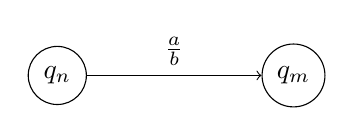
\begin{tikzpicture}[auto, node distance=3cm]
    \node (qn) [circle, draw] {\(q_n\)};
    \node (qm) [circle, draw, right of=qn] {\(q_m\)};

    \path[->] (qn) edge node[above] {\(\frac{a}{b}\)} (qm);
  \end{tikzpicture}
  \caption{Example of a \textit{2I automaton} transition}
  \label{fig:2I-automaton-transition-example}
  \bigskip
\end{figure}

\paragraph{Automaton forms}

By projecting the arc labels of a \textit{2I automaton} on the first component, a new automaton with one input tape is obtained.
The symbols in the tape are from the source alphabet \(\Sigma\) and the input automaton is \textbf{subjacent} to the original machine.

A \textit{2I automaton} in \textbf{normal} form is characterized by the fact that each move reads exactly one character either from the source tape or from the target tape, but not from both.
Arc labels are of the following types:

\begin{enumerate}
  \item label \(\frac{a}{\varepsilon}\) with \(a \in \Sigma\), if one character from source is read
  \item label \(\frac{\varepsilon}{b}\), with \(b \in \Delta\), if one character from target is read
\end{enumerate}

\bigskip
The families of translation defined by \rte and by finite \textit{(eventually nondeterministic)} \textit{2I automata} coincide.

\subsubsection{Nivat Theorem}

The \textbf{Nivat Theorem} states some properties of the transition relation.

\begin{theorem}[Nivat Theorem]
  \label{theo:nivat-theorem}
  The Nivat Theorem states the following \(4\) conditions are equivalent:

  \begin{enumerate}
    \item The translation relation \(\rho_\tau\) is defined by a right-linear \textit{(or left-linear)} translation grammar \(G_\tau\)
    \item The translation relation \(\rho_\tau\) is defined by a \textit{2I-automaton}
    \item The translation relation \(\rho_\tau \subseteq \Sigma^\ast \times \Delta^\ast\) is regular
    \item There exists and alphabet \(\Omega\), a regular language \(R\) over \(\Omega\) and two alphabetic homomorphisms
          \begin{gather*}
            \begin{aligned}
              h_1 : \Omega & \rightarrow \Sigma \cup \left\{ \varepsilon \right\} \\
              h_2 : \Omega & \rightarrow \Delta \cup \left\{ \varepsilon \right\}
            \end{aligned}
          \end{gather*}
          such that:
          \[ \rho_\tau = \left\{ \left( h_1(z), \, h_2(z) \right) \mid z \in R \right\} \]
  \end{enumerate}
\end{theorem}

\subsubsection{Sequential Transducer}

\textbf{Sequential Transducers} are automaton used to efficiently compute the translation in real-time while reading the input tape.
At last, when the input is finished, the automaton may append a finite piece of text that depends on the final state reached.

A formal definition is shown in \textit{(\ref{def:sequential-transducer})}.

\begin{definition}[Sequential Transducer]
  \label{def:sequential-transducer}
  A \textbf{sequential transducer} or \textit{IO-automaton} \(T\) is a deterministic machine defined by a set \(Q\) of states, a source alphabet \(\Sigma\) and a target alphabet \(\Delta\), an initial state \(q_0\) and a set \(F \subseteq Q\) of final states.
  Furthermore, there are three single-valued functions:

  \begin{enumerate}
    \item The state transition function \(\delta\) computes the next state
    \item The output function \(\eta\) computes the string to be emitted by a move
    \item The final function \(\phi\) computes the last suffix to be appended to the target string at termination
  \end{enumerate}

  The domains and images of these three functions are the following:
  \[ \delta: Q \times \Sigma \rightarrow Q \quad \eta: Q \times \Sigma \rightarrow \Delta^\ast \quad \phi : F \times \left\{ \dashv \right\} \rightarrow \Delta^\ast \]
\end{definition}

The graphical representation of the two functions \(\delta(q, a) = r\) and \(\eta(q, a) = u\) is:
\[ q \xrightarrow{\dfrac{a}{u}} r \]
and means that in the state \(q\), while reading character \(a\), emits string \(u\) and move to the next state \(r\).
The final function \(\phi(r, \dashv)\) means that when the source string has been entirely read, if the final state is \(r\), then write string \(v\).

For a source string \(x\), the translation \(\tau(x)\) computed by the sequential transducer \(T\) is the concatenation of two strings, produced by the output function and by the final one:
\[ \left\{ yz \in \Delta^\ast \, \middle\vert \, \exists \ \text{a computation labelled} \ \dfrac{x}{y} \ \text{ending in} \ r \in F \land z = \phi\left( r, \dashv \right) \right\} \]

\bigskip
The machine is deterministic because the input automaton \(\langle Q, \Sigma, \delta, q_0, F \rangle\) belonging to \(T\) is deterministic, and the output and final functions \(\eta\) and \(\phi\) are single-valued.

The condition that the subjacent input automaton is deterministic does not ensure by itself that the translation is single-valued, because between two states of the sequential transducer \(T\) there may be two arcs labelled \(\frac{a}{b}\) and \(\frac{a}{c}\) which cause the output not to be unique.

A function computable via sequential state transducer \textit{(IO-automaton)} is said to be a \textbf{sequential function};
the composition of two sequential functions is a sequential function.

\paragraph{Two opposite passes}

Given a single-valued translation specified by a regular translation expression or by a \textit{2I automaton}, it's not always possible to implement the translation via a sequential transducer such as a deterministic \textit{IO-automaton}.

However, in such cases the translation can be implemented via \textbf{two cascaded} \textit{(deterministic)} \textbf{sequential passes}, each one being one way but scanning the string in opposite directions:

\begin{enumerate}[label=step \arabic*., ref=(step \arabic*), leftmargin=*, widest=step 2.]
  \item a sequential transducer scans \textbf{from left to right} and converts the \textbf{source string} into an intermediate string
  \item another sequential transducer scans the \textbf{intermediate string from right to left} and produces the specified target string
\end{enumerate}

\subsection{Semantic Translation}

None of the previously described syntactic translation methods can handle slightly more complicated translations, such as the translation of the conversion of a number from binary to decimal;
they rely on devices that are too elementary to achieve such goals.

In order to make this kind of translation, a more powerful approach is needed, which is the \textbf{syntax-directed translation}.
The term \textit{directed} marks the difference from the purely syntactic methods explored in the previous Sections.

A semantic technique includes tree-walking procedures, which move along the syntax tree and compute some variables called \textbf{semantic attributes}:
they represent the \textit{meaning} (\textit{or semantic}) of a certain source text.
It's important to notice that a syntax-directed method is not a formal model because attribute computing procedures are not formalized.

A syntax-directed compiler performs two cascaded phases:

\begin{enumerate}[label=\arabic*., ref=(\arabic*)]
  \item\label{enum:syntax-directed-compiler-phase-1} \textbf{Parsing} or syntax analysis
  \item\label{enum:syntax-directed-compiler-phase-2} \textbf{Semantic evaluation} or semantic analysis
\end{enumerate}

Phase~\ref{enum:syntax-directed-compiler-phase-1} computes a syntax tree, usually condensed into an abstract syntax tree, containing the essential information for the next phase.
The semantic phase \textit{\ref{enum:syntax-directed-compiler-phase-2}} consists in applying a set of \textbf{semantic functions} on each node of the tree until all attributes have been evaluated;
the set of evaluated attribute values is the \textbf{meaning} \textit{(or translation)} and it will be found in the root of the tree.

This two-phase approach is called \textbf{two-pass compilation} and it's the most common and simplest method of compilation:
the decoupling of the two phases allows the compiler designer to create them with more freedom.

\subsection{Attribute Grammars}

The meaning of a sentence is a set of attribute values, computed by the semantic functions and assigned to the nodes of the syntax tree.
The syntax-directed translator contains the definition of the semantic functions, which are associated with the grammar rules.
The set of grammar rules and associated semantic functions is called an \textbf{attribute grammar}.

For simplicity, the attribute grammar is defined with respect to an \textbf{abstract syntax}:
a grammar that may be simpler than the real one, with the downside of being often ambiguous.
However, this ambiguity does not prevent a single-valued translation, as the parser will pass to the semantic evaluator only one syntax tree.

Simpler compilers may combine the two phases into a single pass via a unique syntax \textit{(the one of the language)}.

\bigskip
A formal definition of attribute grammar is shown in~\ref{def:attribute-grammar}.

\begin{definition}[Attribute grammar]
  \label{def:attribute-grammar}
  An \textbf{attribute grammar} is defined as follows.

  \begin{enumerate}
    \item A \textbf{context-free syntax} \(G = \left( V, \Sigma, P, S \right)\) where \(V\) and \(\Sigma\) are the terminal and nonterminal sets, \(P\) is the production rule set and \(S\) is the axiom.
          It convenient \textit{(albeit not mandatory)} to avoid having the axiom in any rule \RP.
    \item A \textbf{set of symbols}, the \textit{(semantic)} attributes, associated with nonterminal and terminal syntax symbols.
          The set of the attributes associated with symbol \(\square\) is denoted \(\text{attr}\left( \square \right)\).
          The attribute set of a grammar is partitioned into two disjoint sets, the \textbf{left} and \textbf{right} attributes.
    \item A \textbf{set of semantic functions} \textit{(or rules)}.
          \begin{itemize}
            \item each function is associated with a \textbf{production rule}
                  \[ p: D_0 \rightarrow D_1 D_2 \ldots D_r \quad r \geq 0\]
                  where \(D_0\) is a nonterminal and the other symbols can be \textbf{terminal} or \textbf{nonterminal}
            \item the production \(p\) is called \textbf{syntactic support} of the function and it might be shared between different functions
            \item the attribute \(\sigma\) associated with a symbol \(D_k\) is denoted by \(\sigma_k\) or \(\sigma_D\) if the syntactic symbol occurs exactly once in production \(p\)
            \item a \textbf{semantic function} has the \textbf{form}
                  \[ \sigma_k \coloneqq f \left( \text{attr} \left( \left\{ D_0, D_1, \ldots, D_k \right\} \right) \setminus \left\{ \sigma_k \right\}\right) \quad 0 \leq k \leq r \]
                  function \(f\) assigns to the attribute \(\sigma\) of symbol \(D_k\) the value computed by the function body and its arguments can be any attributes of the same production \(p\), excluding \(\sigma_k\) itself.
            \item normally, semantic functions \textbf{are total in their domain} and written in a suitable notation, called semantic metalanguages. which can be informal
            \item a function \(\sigma_0 \coloneqq f(\ldots)\) defines an \textbf{attribute}, qualified as \textbf{left}, of the nonterminal \(D_0\), which is the \LP \textit{(or parent)} of the production
            \item a function \(\sigma_k \coloneqq f(\ldots), \ k \geq 1\) defines an \textbf{attribute}, qualified as \textbf{right}, of a symbol \textit{(sibling or child)} \(D_k\) occurring in the \RP
            \item the same attribute cannot be in the \textbf{left in a function and right in another}
            \item since terminal characters never occur in the left part, their attributes cannot be of the left type
          \end{itemize}
    \item The set \(\fun(p)\) of functions supported by production \(p\) must satisfy the following \textbf{conditions}:
          \begin{enumerate}[label=\Alph*.]
            \item for each left attribute \(\sigma_0\) of \(D_0\), the exists in \(\fun(p)\) \textbf{exactly one function} defining the attribute
            \item For each right attribute \(\delta_0\) of \(D_0\), \textbf{no function} exists in \(\fun(p)\) defining the attribute
            \item For each left attribute \(\sigma_i, \ i \geq 1\), \textbf{no function }exists in \(\fun(p)\) defining the attribute
            \item For each attribute \(\delta_i, \ i \geq 1\), there exists in \(\fun(p)\) \textbf{exactly one function} defining the attribute
          \end{enumerate}
          \smallskip
          \begin{itemize}
            \item The left attributes \(\sigma_0\) and the right ones \(\delta_i\) with \(i \geq 1\) are called \textbf{internal} for production \(p\) because they are  defined by functions supported by \(p\)
            \item The right attributes \(\delta_0\) and left attributes \(\sigma_i\) with \(i \geq 1\) are called \textbf{external} for production \(p\) because they are defined by functions supported by other productions
          \end{itemize}
    \item Some attributes can be initialized with constant values or with values computed by external functions.
          This is often the case for the so-called lexical attributes, those associated with terminal symbols.
          For such attributes, the grammar does not specify a computation rule.
  \end{enumerate}
\end{definition}

\subsubsection{Dependence Graph}

If the grammar is specified via a translation, it abstracts from the details of tree traversing procedures:
the attribute evaluation program can be automatically constructed from the functional dependencies between attributes, supposing that the bodies of the semantic functions are given.

To prepare for such construction, the functional dependencies are formalized in progressively less abstract ways via directed graphs:

\begin{definition}[Dependence Graph of a Semantic function]
  the nodes of this graph are the arguments and results of the function considered, and there is an arc from each argument to the result.
\end{definition}
\begin{definition}[Dependence Graph of a Production \(p\)]
  this graph, denoted by \(\textit{dep}_p\), collects the dependence graphs for all the functions supported by the production considered.
\end{definition}
\begin{definition}[Dependence Graph of a Decorated Syntax Tree]
  this graph is obtained by pasting together the graphs of the individual productions that are used in the tree nodes.
\end{definition}

\bigskip
A grammar is called \textbf{acyclic} \textit{(or loop-free)} if the dependence graph of the tree is acyclic for every sentence.
A Property relative to the correctness is given in \ref{prop:correctness-attribute-grammar}.

\begin{property}[Correct Attribute Grammar]
  \label{prop:correctness-attribute-grammar}
  Given an attribute grammar satisfying the conditions of Definition \ref{def:attribute-grammar}, the following holds:
  if the attribute dependence graph of the tree is acyclic, the system of equations corresponding to the semantic function has exactly one solution.
\end{property}

Under the acyclicity condition, the equations can be ordered in such a way that each semantic function is applied after the functions that compute its arguments;
this produces a value for the solution since the functions are total.
The solution thus obtained is unique, as in a system of linear equations.

In order to provide a total order of nodes, the topological ordering method can be used.
However, this is a rather inefficient way of computing the solution, since it would be necessary to apply the sorting algorithm even before computing the attribute values.

\bigskip
Checking whether a given grammar is acyclic is another problem.
Since the source language is usually infinite, the acyclicity test cannot be performed by the exhaustive enumeration of all the trees;
an algorithm that determines if an attribute grammar is acyclic exists but is \(\mathcal{NP}\)-complete and thus not used in practice.
It is more convenient to test certain sufficient conditions.

\subsubsection{One-Sweep Semantic Evaluation}

A fast evaluator should be able to compute the values of all the attributes of a tree in a single pass:
a tree can be traversed via a depth-first search, which permits the evaluation of the attributes with just one sweep over the tree.

Let \(N\) be a node of the tree and \(N_1, \ldots, N_r\) its children, while \(t_i\) is the subtree rooted at node \(N_i\).
A depth-first algorithm first visits the tree root.
Then, in order to visit the subtree \(t_N\) rooted at node \(N\), it recursively proceeds as follows:

\begin{enumerate}[label=\arabic*, ref=(\arabic*)]
  \item it performs a depth-first visit of the subtrees \(t_1, \ldots, t_r\) in an order corresponding to some permutation of \(1, \ldots, r\)
  \item evaluates the attributes according to the following principles:
        \begin{itemize}
          \item before entering and evaluating a subtree \(t_N\), it computes the right attributes of node \(N\) \textit{(the root of the subtree)}
                \begin{itemize}[label=\(\rightarrow\)]
                  \item the attributes are then passed as input parameters of the procedure that implements the visit
                  \item procedure calls with input parameters passing are the \inlinequote{descending phase} of the visit
                \end{itemize}
          \item at the end of visit of subtree \(t_N\), it computes the left attributes of node \(N\)
                \begin{itemize}[label=\(\rightarrow\)]
                  \item the attributes are the output parameters of the procedure that implements the visit
                  \item procedure return an output parameter passing are the \inlinequote{ascending phase} of the visit
                \end{itemize}
        \end{itemize}
\end{enumerate}

Not all grammars are compatible with this procedure \textit{(named \textbf{one-sweep})} because more intricate functional dependencies may require several visits of the same node.

An illustration of this procedure is given in Figure \ref{fig:one-sweep}.

\begin{figure}
  \centering
  \bigskip
  \tikzfig{figure-17.tikz}
  \caption{One-sweep semantic evaluation}
  \label{fig:one-sweep}
  \bigskip
\end{figure}

\paragraph{One-Sweep Grammar}
\label{par:one-sweep-grammar}

For each production \(p: D_0 \rightarrow D_1 D_2 \ldots D_r\) with \(r \geq 0\), it's necessary to introduce a new relation between the symbols of the right part of the production.
Then it will be possible to build a directed graph, called \textbf{sibling graph} and denoted by \(\textit{sibl}_p\), that collects the relations between the symbols of the right part of the production \(p\).
The nodes of \(\textit{sibl}_p\) are the symbols \(\left\{ D_1, \ldots, D_r \right\}\) of the production, and has arcs \(D_i \rightarrow D_j\), with \(i \neq j, \ i,j \geq 1\) if in hte dependence graph \(\textit{dep}_p\) there is an arc \(\sigma_i \rightarrow \delta_j\) from an attribute of symbol \(D_i\) to an attribute of symbol \(D_j\).

The nodes of the sibling graph are not the same as those of the dependence graph:
the former are syntactical symbols, the latter are attributes.

The next definition states the conditions that make a grammar suitable for one-sweep evaluation.

\begin{definition}[one-sweep grammar]
  \label{def:one-sweep-grammar-condition}
  A grammar satisfies the one-sweep condition if, for each production \(p : D_0 \rightarrow D_1 D_2 \ldots D_r, \ r \geq 0\) that has a dependence graph \(\textit{dep}_p\), the following clauses hold at the same time:

  \begin{enumerate}[label=\Alph*., ref=(\Alph*)]
    \item\label{enum:one-sweep-grammar-condition-1} Graph \(\textit{dep}_p\) contains no circuit (is acyclic)
    \item\label{enum:one-sweep-grammar-condition-2} Graph \(\textit{dep}_p\) does not contain a path \(\lambda_i \rightarrow \ldots \rightarrow \rho_i, \ i \geq 1\) that goes from a left attribute \(\lambda_i\) to a right attribute \(\rho_i\) of the same symbol \(D_i\), where \(D_i\) is a sibling of \(D_0\)
    \item\label{enum:one-sweep-grammar-condition-3} Graph \(\textit{dep}_p\) contains no arc \(\lambda_0 \rightarrow \rho_i, \ \geq 1\), from a left attribute of the father node \(D_0\) to a right attribute of a sibling node \(D_i\)
    \item\label{enum:one-sweep-grammar-condition-4} The sibling graph \(\textit{sibl}_p\) contains no circuit (is acyclic)
  \end{enumerate}
\end{definition}

\subparagraph*{Explanation of the conditions}

\begin{enumerate}
  \item[\ref{enum:one-sweep-grammar-condition-1}] necessary for the grammar to be acyclic
  \item[\ref{enum:one-sweep-grammar-condition-2}] if such a path existed, it would be impossible to compute the right attribute \(\rho_i\) before visiting the subtree \(t_i\), because the value of the left attribute \(\lambda_i\) is computed at the end of the visit of \(t_i\) (against the order of the depth-first visit)
  \item[\ref{enum:one-sweep-grammar-condition-3}] the value of attribute \(\rho_i\) would not be available when the visit of the subtree \(t_i\) is started
  \item[\ref{enum:one-sweep-grammar-condition-4}] allows to topologically sort the child nodes
\end{enumerate}

\paragraph{Construction of the One-Sweep Evaluator}

The procedure visits the subtrees, computes, and returns the left attributes of the root of the subtree.
For each production \(p : D_0 \rightarrow D_1 D_2 \ldots D_r, \ r \geq 0\):

\begin{enumerate}
  \item choose a topological order \textit{(TOS)} of the nonterminals \(D_1, D_2, \ldots \, D_r\) with respect ot the sibling graph \(\textit{sibl}_p\)
  \item for each symbol \(D_i, \ 1 \leq i \leq r\), choose a topological order \textit{(TOR)} of the right attributes of symbol \(D_i\) with respect to the dependence graph \(\textit{dep}_p\)
  \item choose a topological order \textit{(TOL)} of the left attributes of symbol \(D_0\) with respect to the dependence graph \(\textit{dep}_p\)
\end{enumerate}

The three orders \textit{TOS}, \textit{TOR} and \textit{TOL} prescribe how to arrange the instructions of the procedure that implements the visit of the subtree \(t_N\).

\bigskip
\textit{To better understand the procedure, check the example on Page 454 of the textbook.}

\subsubsection{Combined Syntax and Semantic Analisys}

It's possible to combine syntax tree construction and attribute computation, trusting the parser with the duty to invoke the semantic functions.
In the following consideration, a pure \textit{BNF} grammar is assumed, as using the \EBNF productions would make it more complicated to specify the correspondence between syntax symbols and attributes.
There are three typical situations for the analysis, depending on the nature of the source language, shown in Table~\ref{tab:combined-syntax-and-semantic-analysis}.

\begin{table}[htbp]
  \centering
  \bigskip
  \begin{tblr}{colspec={c|c|c}, row{1}={font=\itshape}, cell{2,4}{3}={font=\ttfamily}, cell{3,4}{1}={mode=math}}
    source language & analysis                                 & tool        \\
    \hline
    regular         & lexical analysis with lexical attributes & flex, lex   \\
    LL(k)           & recursive descent parser with attributes &             \\
    LR(k)           & shift-reduce parser with attributes      & yacc, bison
  \end{tblr}
  \caption{Combined syntax and semantic analysis}
  \label{tab:combined-syntax-and-semantic-analysis}
  \bigskip
\end{table}

\paragraph{Lexical Analysis with Attribute Evaluation}

The \textbf{lexical analyser} \textit{(or scanner)} segments the source text into the lexical elements, called \textbf{lexemes} \textit{(or tokens)}, such as identifiers, integers and strings;
lexemes are the smallest substrings that can be invested with some semantic meaning.
Each technical language uses a finite set of lexical classes, represented by regular formal language, like a regular expression or a set of strings.

Technical languages have two different levels of syntactic specifications:
\begin{itemize}
  \item \textbf{lexical} \textit{(lower)}, defining the form of the lexemes
  \item \textbf{syntactic} \textit{(higher)}, assuming that the lexemes are given, and considering them as terminal symbols of the grammar
\end{itemize}

Some lexemes may carry meaning, like a semantic attribute, that is computed by the lexical analyser.

\subparagraph{Attributed Recursive Descent Translator}

Assuming that a syntax is suitable for deterministic top-down parsing \textit{(as shown in Section~\ref{sec:top-down})}, the attribute evaluation can proceed with parsing if the functional dependencies of the grammar obey additional conditions beyond the one-sweep grammar conditions:

\begin{itemize}
  \item the one-sweep algorithm visits in depth-first order the syntax tree, in an order that can be different from the natural one
  \item the top-down parser constructs the tree in the natural order
\end{itemize}

In order to combine the two procedures is necessary to exclude any functional dependency that would make the two procedures visit the tree in different orders, as stated in Definition~\ref{def:l-condition}.

\begin{definition}[L-condition]
  \label{def:l-condition}
  A grammar satisfies the condition \textbf{L} if, for each production \(p: D_0 \rightarrow D_1 \ldots D_r\), it holds:

  \begin{enumerate}[label=\alph*., ref=(\alph*)]
    \item\label{enum:l-condition-1} The one-sweep condition \textit{(Definition~\ref{def:one-sweep-grammar-condition})} is satisfied
    \item\label{enum:l-condition-2} The sibling graph \(\textit{sibl}_p\) \textit{(Paragraph~\ref{par:one-sweep-grammar})} contains arc \(D_j \rightarrow D_i, \ j > i \geq 1\)
  \end{enumerate}
\end{definition}

The condition \ref{enum:l-condition-2} prevents a right attribute of node \(D_i\) to depend from any attribute of a node \(D_j\) placed to its \textbf{right} in the production \(p\).

\bigskip
The next Property \textit{(\ref{def:attribute-grammar-and-deterministic-parsing})} relates the \textit{L-condition} and deterministic parsing.

\begin{definition}[Attribute Grammar and Deterministic Parsing]
  \label{def:attribute-grammar-and-deterministic-parsing}
  Consider an attribute grammar \(G\), where:

  \begin{itemize}
    \item the syntax satisfies the \(LL(k)\) condition
    \item the semantic rules satisfy the L-condition
  \end{itemize}

  It's possible to construct a top-down deterministic parser with attribute evaluation able to compute the attributes of \(G\) at parsing time.
\end{definition}

\subsection{Static Analysis}

Static analysis is a technique used by compilers to check some properties of the source code, before the compilation phase.
The different analyses are categorized according to the purpose of the check, for example:

\begin{itemize}
  \item \textbf{verification}, to examine the program correctness
  \item optimization, to improve the efficiency of the program
  \item \textbf{scheduling} and parallelizing, to change the execution order of the program in order to exploit the parallelism
\end{itemize}

Such cases use a \textbf{control-flow graph}, a directed graph similar to a program flowchart.
It's convenient to view this graph as describing the state-transition function of a finite automaton:
static analysis is performed by analysing it, using various techniques.

It's important to notice that the control-flow graph does not represent the entire source language, but only the source code of a single program:
static flow analysis must not be confused with syntax-driven translation.

\subsubsection{Program as an Automaton}

The control-flow graph is an abstraction of a program, that can be represented by a \FSA;
its component is now described.

\begin{itemize}
  \item Each \textbf{node} represent an instruction
        \begin{itemize}
          \item the instructions are simpler than the ones of the source language
          \item typical instructions are assignment, jump, arithmetic operations, \ldots
          \item the operands are all simple variables and constants
        \end{itemize}
  \item Each \textbf{arc} represents a \textbf{possible control flow}
        \begin{itemize}
          \item if an instruction \(p\) is followed by \(q\), there is a directed \textbf{arc} from \(p\) to \(q\)
          \item \textbf{unconditional} instructions have at \textbf{most one successor}
          \item \textbf{conditional} instructions have \textbf{two \textit{(or more)} successors}
          \item an \textbf{instructions} with two or more \textbf{predecessors} is a \textbf{confluence of arcs} in the graph
        \end{itemize}
  \item The \textbf{first instruction} of the program is the entry point and corresponds to the \textbf{initial node}
  \item The \textbf{last instruction} of the program is the exit point and corresponds to the \textbf{final node}
\end{itemize}

A control-flow graph is not a faithful representation of the program, as it misses:

\begin{itemize}
  \item the \texttt{true}/\texttt{false} value determining the successor of a conditional instruction
  \item the node representing a \texttt{goto} instruction, as it's just an arc to the successor instruction
  \item any operation performed by an instruction, as they are replaced by an abstraction
        \begin{itemize}
          \item a value assignment is said to define a variable
          \item if a variable occurs in the \RP of an expression or boolean condition, it's said to be \textbf{used}
          \item a node representing a statement \(p\) in the graph is associated with \textbf{set} \(\text{def}(p)\) of \textbf{defined variables} and \textbf{set} \(\text{use}(p)\) of \textbf{used variables}
        \end{itemize}
\end{itemize}

\subparagraph*{Language of the control-flow graph}
The language of the control-flow graph is defined in~\ref{def:control-flow-graph}.

\begin{definition}[Language of the control-flow graph]
  \label{def:control-flow-graph}
  Let \(A\) be a finite state automaton, represented by a control-flow graph.
  Its terminal alphabet is the set \(I\) of program instructions, each represented by a \(3\)-tuple:
  \[ \left\langle \texttt{label},\ \texttt{defined variables},\ \texttt{used variables} \right\rangle \]
  The language \(L(A)\) recognized by the automaton contains the strings over the alphabet \(I\) that label the paths from the initial node \textit{(the entry point)} to the final node \textit{(the exit point)}:
  its strings represent a sequence of program instructions the machine can execute when the program is run.
\end{definition}

Furthermore, language \(L\) is \textbf{local} \textit{(Definition~\ref{def:local-language})}.

\subparagraph*{Conservative approximation}

The automaton can specify only an approximation of the valid execution path of a program.
Not all paths are executable by the program, as no syntax analysis is performed on the conditions selecting the successor's nodes in conditional instructions.
For example, consider the following instruction.
\[ 1: \texttt{if} \ a^2 \geq 0 \ \texttt{then} \ 2: \ \textit{instruction}_2 \ \texttt{else} \ 3: \ \textit{instruction}_3 \]
The formal language accepted by the automaton contains two paths:
\[ \left\{ 1 \, 2, \ 1 \, 3 \right\} \]
even though the second path is not executable, as the condition is always true.

As a consequence, static analysis may sometimes reach pessimistic conclusions \textit{(it may discover never executed code paths)}.
It's not decidable whether a path of a control-flow graph will ever be executed by the program, as the problem can be reduced to the halting problem.

The decision to analyze all recognized paths is a conservative approximation to program analysis:
it might diagnose non-existing errors or erroneously assign resources, but real errors will never be missed.
The method is then defined as \textbf{error safe}, despite being possibly inefficient.

A usual hypothesis in static analysis is that the automaton is clean \textit{(Section~\ref{sec:clean-automaton}, page~\pageref{sec:clean-automaton})}, and every instruction is on a path from the entry point to the exit point.
If this is not the case, anomalies may happen:

\begin{itemize}
  \item some executions don't reach the exit point
  \item some instructions are never executed \textit{(dead code)}
\end{itemize}

\subsubsection{Liveness of a variable}

A professional compiler performs several passes of analysis, in order to optimize the code.
One of the most important is the analysis of \textbf{variable liveness} \textit{(Definition~\ref{def:variable-liveness})} that determines how long the value of a variable is needed.

\begin{definition}[Variable liveness]
  \label{def:variable-liveness}
  A variable \(a\) is \textbf{live} on the exit from a program node \(p\) if in the program control-flow graph there exists a path from \(p\) to a node \(q\) \textit{(not necessarily distinct from \(p\))} such that:
  \begin{itemize}
    \item the path does not traverse an instruction \(r \neq q\) that define \(a\)
          \begin{itemize}[label=\(\rightarrow\)]
            \item if \(r\) defines \(a\), then \(a \in \text{def}\left(r\right)\)
          \end{itemize}
    \item instruction \(q\) uses \(a\)
          \begin{itemize}[label=\(\rightarrow\)]
            \item if \(q\) uses \(a\), then \(a \in \text{use}\left(q\right)\)
          \end{itemize}
  \end{itemize}
  For brevity, the variable liveness condition is called \textbf{live out}.
\end{definition}

In other words, a variable is live-out of a certain node if some instruction that may be successively executed makes use of the value that variable has in the former node.
If the variable gets reassigned before the next use, it's not live-out of the node.

More precisely, a variable is \textbf{live-out} for a node if it is live on any \textbf{arc leaving} from that node.
Similarly, a variable is \textbf{live-in} for a node if it is live on some \textbf{arc entering} the node.

\subparagraph*{Computing Liveness Intervals}

Let \(I\) be the instruction set.
Let \(D(a)(I) \subseteq I\) and \(U(a)(I) \subseteq I\) be the sets of instructions that define and use variable \(a\), respectively.

Variable \(a\) is live-out of an instruction \(p\) if and only if for the language \(L(A)\) accepted by the automaton, the following condition holds:
language \(L(A)\) contains a sentence \(x = u p v q w\), where:
\begin{itemize}
  \item \(u, \ w\) are arbitrary sequences of instructions \textit{(possibly empty)}
  \item \(p\) is any instruction
  \item \(v\) is a possibly empty instruction sequence not containing a definition of \(a\)
  \item \(q\) is an instruction that uses \(a\)
\end{itemize}

The above conditions are formalized by the equation:
\[ u, w \in I^\ast \land p \in I \land v \in \left( I \setminus D\left( a \right) \right) \land q \in U\left( a \right) \]
The set difference contains all the instructions that do not define \(a\), while \(q\) uses \(a\).
The set of all strings \(x\) that meet this condition, defined as \(L_p\), is a subset of the language \(L(A)\) recognized by the automaton.
Language \(L_p\) is regular because it can be defined by the following intersection:
\[ L_p = L(A) \cap R_p \]
where \(R_p\) is the regular language defined by the regular expression:
\[ R_p = I^\ast p \left( I \setminus D \left( a \right) \right)^\ast U \left( a \right) I^\ast \]
The definition of \(R_p\) and \(L_p\) prescribe that letter \(p\) must be followed by a letter \(q\) taken from set \(U\left( a \right)\)  and all the letter between \(p\) and \(q\) must not be in set \(D\left( a \right)\).

To check if a variable is a live-out of node \(p\), it is sufficient to check if \(L_p \neq \emptyset\);
to achieve that goal it's sufficient to build the recognizer as the product of machine \(A\) and the recognizer of \(R_p\).
If no path connecting the input node to the final node exists, then \(L_p\) is empty.

Such a procedure is however not efficient, considering the big number of variables and instructions in real-world programs;
a more efficient technique is the \textbf{data-flow analysis}.
This method examines all paths from any instruction to another instruction that uses the same variable.

The liveness computation is expressed as a system of data-flow equations:
consider a node \(p\) of a program \(A\).
A first equation expresses the relation between the variables live-out \(\text{live}_\text{out}\left( p \right)\) and those live-in \(\text{live}_\text{in}\left( p \right)\) of the node;
a second equation expresses the relation between the variables live-out of a node and those live-in for its successors.
\(\text{succ}\left( p \right)\) denotes the set of \textit{(eventually immediate)} successors of node \(p\) and by \(\text{var}(A)\) the set of all the variables of program \(A\).

The equations are shown in Definition~\ref{def:data-flow-equations}.

\begin{definition}[Data-Flow Equations]
  \label{def:data-flow-equations}
  For each final node \(p\):
  \[ \text{live}_\text{out}\left( p \right) = \emptyset \]
  For any other node \(p\):
  \[ \text{live}_\text{in}\left( p \right) = \text{use}\left( p \right) \cup \left( \text{live}_\text{out} \left( p \right) \leq \text{def}\left( p \right) \right) \]
  \[ \text{live}_\text{out}\left( p \right) = \bigcup_{q \in \text{succ}\left( p \right)} \text{live}_\text{in}\left( q \right) \]
\end{definition}

\paragraph{Solution of Data-Flow Equations}

Given a control-flow graph with a number \(|I| = n \geq 1\) of nodes, the resulting system has \(2 \cdot n\) equations with \(2 \cdot n\) unknown variables: \(\text{live}_\text{in}\left( p \right)\) and \(\text{live}_\text{out}\left( p \right)\) for each node \(p \in I\).
Each unknown is a set of variables, and the solution to be computed is a pair of vectors, each one containing \(n\) sets.

To solve the system of equations, the following iteration is used, by taking the empty set as the initial approximation \textit{(\(i=0\))} for every unknown:
\[ \forall \, p \in I \quad \text{live}_\text{in}\left( p \right) = \emptyset \quad \text{live}_\text{out} \left( p \right) = \emptyset \]
At any iteration \(i\), for each equation of the system in \ref{def:data-flow-equations}, the unknowns in the right-hand side are replaced with the values computed in the previous iteration;
the new iteration \(i + 1\) is then calculated.

The iteration stops when the values computed in the last iteration are equal to those computed in the previous iteration \textit{(a fixed point is reached)};
this solution is termed the \textbf{least fixed point solution} of the transformation that computes a new vector from one of the preceding iterations.

A finite number of iterations is always sufficient to compute the least fixed point solution, because:

\begin{itemize}
  \item every set \(\text{live}_\text{in}\left( p \right)\) and \(\text{live}_\text{out}\left( p \right)\) is finite \textit{(the number of variables is finite)}
  \item every iteration step either increases the cardinality of the above sets of variables or leaves them unchanged, as the equation is monotonic
  \item when the solution does not change anymore, the algorithm terminates
\end{itemize}

\paragraph{Application of Liveness Analysis}

\subparagraph*{Memory allocation}

Liveness analysis is best applied to decide if two variables can reside in the same memory cell:
if two variables are live-in in the same program instruction, then both variables must be stored in different memory cells.
The two variables then \textbf{interfere}.

Conversely, if two variables do not \textbf{interfere}, then they can be stored in the same memory cell.

\subparagraph*{Useless instructions}

An instruction defining a variable is \textbf{useless} is the value assigned to the variable that is never used by any instruction:
the value is not live-out for the defining instruction.
Therefore, to verify that the definition of a variable \(a\) by instruction \(p\) is useless, it is sufficient to check if \(\text{live}_\text{out}\left( p \right) \not\subseteq \left\{ a \right\}\).

\subsubsection{Reaching Definition Analysis}

Another basic applied type of static analysis is the search for a variable definition that reaches a given instruction.

Consider an instruction that assigns a constant value to variable \(a\).
The compiler examines the program to see if the same constant can be replaced for the variable in the instructions using \(a\), with the advantage of:

\begin{enumerate}[label=\arabic*., ref=\arabic*.]
  \item\label{enum:reaching-definition-analysis-1} replacing the variable with a constant value, reducing the number of memory accesses and increasing the speed of the program
  \item\label{enum:reaching-definition-analysis-2} obtaining an expression where all the operands are constant, which can be evaluated at compile time
\end{enumerate}

The transformation \ref{enum:reaching-definition-analysis-2} is termed \textbf{constant propagation} and will be analysed later \textit{(\ref{par:constant-propagation})}.

A formal definition of the Reaching Definition problem is given in~\ref{def:reaching-definition}.

\begin{definition}[Reaching Definition]
  \label{def:reaching-definition}
  The \textbf{definition} of a variable \(a\) at instruction \(q\) \textit{(denoted as \(a_q\))} \textbf{reaches} the input of an instruction \(p\) (not necessarily different from \(q\)) if there exists a path from \(q\) to \(p\) that does not contain any redefinition of \(a\).
\end{definition}

Instruction \(p\) can then see and use the value of the variable \(a\) defined in instruction \(q\).

Given an automaton \(A\) with instruction set \(I\), the Definition~\ref{def:reaching-definition} can be expressed as a regular expression over the language \(L(A)\) or via a system of data-flow equations.

\begin{definition}[Reaching Definition, via regular expression]
  \label{def:reaching-definition-regular-expression}
  Definition \(a_q\) reaches instruction \(p\) if language \(L(A)\) contains a sentence of the form \(x = u q v p w\), where:
  \begin{itemize}
    \item \(u, \ w\) are arbitrary sequence of instructions \textit{(possibly empty)}
    \item \(p\) is any instruction
    \item \(v\) is a sequence of instructions that do not contain any definition of \(a\) \textit{(possibly empty)}
    \item \(q\) is an instruction that defines \(a\)
  \end{itemize}

  This condition is represented via the following regular expression:
  \[ u, \ w \in I^\ast \land q \in D\left( a \right) \land v \in \left( I \setminus D \left( a \right)\right)^\ast \land p \in I \]
  where \(p, \ q\) may coincide.
\end{definition}

\begin{definition}[Reaching Definition, via data-flow equations]
  \label{def:reaching-definition-data-flow-equations}
  If node \(p\) defines variable \(a\), any other definition \(a_q\) of the same variable in another node \(q\), with \(q \neq p\) is \textbf{suppressed} by \(p\).
  The set of definitions suppressed by instruction \(p\) is the following:
  \[\begin{cases}
      \text{sup}(p) = \emptyset \quad                                                                                             & \text{if} \ \text{def}(p) = \emptyset    \\
      \text{sup}(p) = \left\{ a_q \mid q \in I \land q \neq p \land a \in \text{def} (q) \land a \in \text{def}(p) \right\} \quad & \text{if} \ \text{def}(p) \neq \emptyset
    \end{cases}\]
\end{definition}

\subparagraph*{Data-Flow Equations}

For the initial node \(1\):
\[
  \label{eq:reaching-definition-data-flow-equations-1}\tag{A}\text{in}(1) = \emptyset
\]
For any other node \(p \in I\):
\[
  \label{eq:reaching-definition-data-flow-equations-2}\tag{B}\text{out}(p) = \text{def}(p) \cup \left( \text{in}(p) \setminus \text{sup}(p) \right)
\]
\[
  \label{eq:reaching-definition-data-flow-equations-3}\tag{C}\text{in}(p) = \bigcup_{\forall \, q \, \in \, \text{pred}(p)} \text{out}(q)
\]

Similarly to the liveness equations \textit{(Definition~\ref{def:variable-liveness})}, the reaching definition system can be solved by iteration until the computed solution converges to a fixed point;
initially, all sets are empty.

\bigskip
The set \(\text{out}^\prime\) denotes the elements of \(\text{out}\) reaching the exit node starting from node \(q\), but with their subscripts deleted.

\subparagraph*{Explanation}

\begin{itemize}
  \item Equation \ref{eq:reaching-definition-data-flow-equations-1} assumes that no variable is passed as input parameters to the subprogram
        \begin{itemize}[label=\(\rightarrow\)]
          \item otherwise, \(\text{in}(1)\) would be the set of input parameters
        \end{itemize}
  \item Equation \ref{eq:reaching-definition-data-flow-equations-2} inserts into exit from \(p\) all the local definitions of \(p\) and the definitions reaching the entrance to \(p\), provided the latter are not suppressed by \(p\)
  \item Equation \ref{eq:reaching-definition-data-flow-equations-3} states that any definition reaching the exit of some predecessor node reaches also the entrance to \(p\)
\end{itemize}

\paragraph{Constant Propagation}
\label{par:constant-propagation}

The constant propagation problem is the search for constant expressions that can be evaluated at compile time.

\begin{definition}[Constant Propagation]
  \label{def:constant-propagation}
  In the instruction \(p\), it is safe to replace with a constant \(k\) any variable \(a\) used in \(p\) if the following conditions hold:

  \begin{enumerate}
    \item There exists and instruction \(q : a \coloneqq k\), such that \(a_q\) reaches \(p\)
    \item No other definition \(a_r\) of variable \(a\) reaches the entrance of \(p\), with \(r \neq q\)
  \end{enumerate}
\end{definition}

\paragraph{Availability of Variables and Initialization}

A basic correctness check performed by a compiler is to verify that all the variables are initialized before their first use;
more generally, a variable used in some instruction must be available at the entrance of that instruction.

A definition of availability is shown in Definition~\ref{def:variable-availability}, under the assumption that the subprogram has no input parameters.

\begin{definition}[Variable Availability]
  \label{def:variable-availability}
  A variable \(a\) is \textbf{available} at the entrance of instruction \(p\) \textit{(just before its execution)} if in the program control-flow graph every path from the initial node \(1\) to the entrance of \(p\) contains a statement that defines variable \(a\).
\end{definition}

\paragraph{Badly Initialized Variables}

A formal definition of badly initialized variables is given in~\ref{def:badly-initialized-variables}.

\begin{definition}[Badly Initialized Variables]
  \label{def:badly-initialized-variables}
  An instruction \(p\) is not well initialized if the following predicate holds:
  \[ \exists \, q \in \text{pred}(p) \ \text{such that} \ use(p) \nsubseteq \text{out}^\prime(q) \]
\end{definition}

The condition says that there exists a node \(q\) predecessor of \(p\) such that the definition of reaching its exit does not include all the variables used in \(p\).
Therefore, when the program execution runs on a path through \(q\), one or more variables used in \(p\) don't have a value.

\clearpage

\section{Laboratory}

The laboratory has the following requirements:

\begin{enumerate}
  \item Familiarity of the \clang programming language
  \item Being able to use a standard \texttt{UNIX} compilation toolchain
  \item Know how a \clang \texttt{struct} is represented in memory
\end{enumerate}

\subsection{Regular Expressions}

The \texttt{POSIX} compatible regular expression library is a standard library of the \clang programming language.
It contains an extended set of functions to build and manipulate regular expressions.

Table~\ref{tab:basic-character-sets} shows the basic character sets used in regular expressions, Table~\ref{tab:regular-expression-composition-rules} shows the composition rules of regular expressions, and Table~\ref{tab:regular-expression-utilities} shows some useful sets of characters.

\begin{table}[htbp]
  \centering
  \bigskip
  \begin{tblr}{colspec={c|l}, row{1}={font=\itshape}}
    syntax                            & matches                                       \\
    \hline
    \texttt{x}                        & the character \texttt{x}                      \\
    \texttt{.}                        & any character except newline                  \\
    \texttt{[x,y,z]}                  & any character in the set \texttt{x, y, z}     \\
    \texttt{[\textasciicircum x,y,z]} & any character not in the set \texttt{x, y, z} \\
    \texttt{[a-z]}                    & any character in the range \texttt{a-z}       \\
    \texttt{[\textasciicircum a-z]}   & any character not in the range \texttt{a-z}   \\
  \end{tblr}
  \caption{Basic character sets}
  \label{tab:basic-character-sets}
  \bigskip
\end{table}

\begin{table}[htbp]
  \centering
  \bigskip
  \begin{tblr}{colspec={c|l}, row{1}={font=\itshape}}
    syntax                & matches                                                              \\
    \hline
    \texttt{R}            & the regular expression \texttt{R}                                    \\
    \texttt{R S}          & the concatenation of \texttt{R} and \texttt{S}                       \\
    \texttt{R\textbar{}S} & the alternation of \texttt{R} and \texttt{S}                         \\
    \texttt{R*}           & zero or more occurrences of \texttt{R}                               \\
    \texttt{R+}           & one or more occurrences of \texttt{R}                                \\
    \texttt{R?}           & zero or one occurrence of \texttt{R}                                 \\
    \texttt{R\{n\}}       & exactly \texttt{n} occurrences of \texttt{R}                         \\
    \texttt{R\{n,\}}      & at least \texttt{n} occurrences of \texttt{R}                        \\
    \texttt{R\{n,m\}}     & at least \texttt{n} and at most \texttt{m} occurrences of \texttt{R} \\
  \end{tblr}
  \caption{Composition of Regular Expressions}
  \label{tab:regular-expression-composition-rules}
\end{table}

\begin{table}[htbp]
  \centering
  \bigskip
  \begin{tblr}{colspec={c|l}, row{1}={font=\itshape}}
    syntax                      & matches                                                                                         \\
    \hline
    \texttt{(R)}                & capture group or override precedence                                                            \\
    \texttt{\textasciicircum R} & match at the beginning of the line                                                              \\
    \texttt{R\$}                & match at the end of the line                                                                    \\
    \texttt{\textbackslash t}   & tab character                                                                                   \\
    \texttt{\textbackslash n}   & newline character                                                                               \\
    \texttt{\textbackslash w}   & a word (same as \texttt{[a-zA-Z0-9\_]})                                                         \\
    \texttt{\textbackslash d}   & a digit (same as \texttt{[0-9]})                                                                \\
    \texttt{\textbackslash s}   & a whitespace character (same as \texttt{[ \textbackslash t \textbackslash s \textbackslash n]}) \\
    \texttt{\textbackslash W}   & a non-word character                                                                            \\
    \texttt{\textbackslash D}   & a non-digit character                                                                           \\
    \texttt{\textbackslash S}   & a non-whitespace character                                                                      \\
  \end{tblr}
  \caption{Regular expression utilities}
  \label{tab:regular-expression-utilities}
  \bigskip
\end{table}

\subsection{Lexical Analysis}

The purpose of the lexical analysis is:

\begin{enumerate}
  \item to \textbf{recognize} the tokens of the language
  \item to \textit{(possibly)} \textbf{decorate} the tokes with additional informations
\end{enumerate}

Such analysis is performed through a scanner, which is a big \FSA.
Since coding a scanner is a hard task, scanner generators based on regular expressions such as \flex are used.

In a compiler, the scanner prepares the input for the parser:

\begin{enumerate}
  \item it detects the tokens of the language
  \item it cleans the input
  \item it adds information to the tokens
\end{enumerate}

\subparagraph*{Words}
Words cannot be enumerated in artificial languages, as there are too many of them \textit{(despite being bounded)}.
However, technical words are simpler than natural words:

\begin{itemize}
  \item Their structure is simple
  \item They follow specific rules
  \item They are \textit{(normally)} a regular language
\end{itemize}

\begin{property}[\clang identifiers]
  \label{prop:c-identifiers}
  \hfill
  \begin{enumerate}
    \item The \textbf{first} character must be a \textbf{letter} or an \textbf{underscore}
    \item The \textbf{following} characters must be \textbf{letters}, \textbf{digits} or \textbf{underscores}
  \end{enumerate}
\end{property}

\subparagraph*{\flex}
\flex is a lexical analyser generator:

\begin{itemize}
  \item[\(\rightarrow\)] as \textbf{input} it takes a specification file of the scanner
  \item[\(\leftarrow\)] as \textbf{output} it generates a \clang source code file implementing the scanner
\end{itemize}

The workflow of \flex \textit{(illustrated in Figure~\ref{fig:flex-workflow})} is the following:

\begin{enumerate}
  \item The \textbf{specification} file is \textbf{written}
  \item The \textbf{specification} file is \textbf{compiled} with \texttt{FLEX}
  \item The \textbf{generated} \clang source code file is \textbf{compiled} with \texttt{cc}
\end{enumerate}

\begin{figure}[htbp]
  \centering
  \bigskip
  \tikzfig{figure-18.tikz}
  \caption{Workflow of \flex}
  \label{fig:flex-workflow}
  \bigskip
\end{figure}

The generated parsers implement a nondeterministic \FSA, later made deterministic via the Berry-Sethi algorithm, which tries to match all possible tokens at the same time;
as soon as one is recognized:

\begin{enumerate}
  \item The semantic action is executed
  \item The stream skips past the end of the token
  \item The automaton reboots
\end{enumerate}

\subsubsection{Specification File}

A \flex file is structured in three sections, separated by the \texttt{\%\%} token:

\begin{itemize}
  \item the \textbf{definitions}: declare useful \re
  \item the \textbf{rules}: bind \re combinations to actions
  \item the \textbf{user code}: \clang code
\end{itemize}

\subparagraph*{Definitions}
A definition associates a name with a set of characters;
\re can be used to define character sets, with quotes \textit{(symbol \texttt{"})} used for literal strings.
They are recalled by putting their names in curly braces \textit{(symbol \texttt{\{\}})}.
Definitions behave like \clang macros.

\subparagraph*{Rules}
A rule represents a full token to be recognized:

\begin{itemize}
  \item the \textbf{token} is described by a \re
  \item it exploits definitions to be more readable
  \item it defines a \textbf{semantic action} to be made at each match
        \begin{itemize}
          \item semantic actions are executed \textbf{every time the rules matches} and can access the matched string
          \item global variables:
                \begin{itemize}[label=\texttt{>}]
                  \item \texttt{\textbf{char} *yytext} contains the \textbf{matched string}
                  \item \texttt{\textbf{int} yyleng} contains the \textbf{length of the matched string}
                \end{itemize}
        \end{itemize}
\end{itemize}

Simple applications put the business logic inside the semantic actions;
more complex applications that use a separate parser \textit{(for example compilers)} do the following:

\begin{enumerate}
  \item \textbf{assign} a \textbf{value} to the recognized token
  \item \textbf{return} the token \textbf{type}
\end{enumerate}

\subparagraph*{User Code}

User \clang code is copied to the generated scanner \textbf{as is}.

Arbitrary code can be put inside definitions and rules sections by escaping from the \flex syntax within \texttt{\%\{} and \texttt{\%\}}.
This feature is usually used for header inclusions, global variables, and function definitions.

\subsubsection{Generated Scanner}

While \flex generates a scanner, \textbf{it is not a scanner itself};
the generated scanner is a \clang source code file called \texttt{lex.yy.c}, exporting the following variables and functions:

\begin{itemize}[label=\texttt{>}]
  \item \texttt{\textbf{FILE} *yyin}: the input file
        \begin{itemize}
          \item it can assume the value \texttt{stdin} to read from the standard input
        \end{itemize}
  \item \texttt{\textbf{int} yylex(\textbf{void})}
        \begin{itemize}
          \item it parses the input until:
                \begin{enumerate}
                  \item a semantic function returns; the return value is the same as the one in the action
                  \item the file ends; the return value is \texttt{0}
                \end{enumerate}
        \end{itemize}
  \item \texttt{\textbf{void} yyerror(\textbf{char} *msg)}
        \begin{itemize}
          \item prints an error message
        \end{itemize}
  \item \texttt{\textbf{int} yywrap(\textbf{void})}
        \begin{itemize}
          \item it is called when the end of the file is reached
          \item it allows opening a new file and continue scanning from there
          \item return values:
                \begin{itemize}
                  \item \texttt{0}: continue scanning
                  \item \texttt{1}: stop scanning
                \end{itemize}
          \item it can be disabled with the instruction \texttt{\%\%option noyywrap} in the specification file
        \end{itemize}
\end{itemize}

\subparagraph*{Behaviour}
Important behaviours of the scanner:

\begin{itemize}
  \item \textbf{Longest matching rule} - if the scanner matches \textbf{more than one string}, the rules that generates the \textbf{longest} one is chosen
  \item \textbf{First rule} - if the scanner matches\textbf{ more than one string with the same length}, the \textbf{first} one is chosen
  \item \textbf{Default action} - if the scanner finds no rule, the next character in input is considered matched implicitly and printed to the standard output
\end{itemize}

\subsubsection{Multiple scanners}

In order to support multiple scanners, rules can be marked with the same name of the associated scanner \textit{(the start condition)};
special actions are used to switch between scanners.

A start condition \texttt{S} is used to mark rules with as a prefix like \texttt{<S>RULE};
it marks rules as active when the scanner is running the scanner \texttt{S}.

\begin{itemize}
  \item The \texttt{*} start condition matches every start condition
  \item The initial start condition is called \texttt{INITIAL}
  \item The start conditions are stored as integers
  \item The current start condition is stored in the variable \texttt{YY\_START}
\end{itemize}

\bigskip
Start conditions can be:

\begin{itemize}[label=\texttt{>}]
  \item \textbf{exclusive} - declared as \texttt{\%x S;}
        \begin{itemize}
          \item \textbf{disables unmarked rules} when the scanner is in the start condition \texttt{S}
        \end{itemize}
  \item \textbf{inclusive} - declared as \texttt{\%s S;}
        \begin{itemize}
          \item \textbf{enables unmarked rules} when the scanner is in the start condition \texttt{S}
          \item the \texttt{INITIAL} condition is inclusive
        \end{itemize}
\end{itemize}

Command \texttt{BEGIN(S)} switches to the start condition \texttt{S};
command \texttt{ECHO} copies the content of the matched string \texttt{yytext} to the standard output.

\subsection{Syntactic Analysis - \bison}

The purpose of the Syntactic Analysis is:

\begin{enumerate}
  \item identify the grammar structures of the input
  \item verify the syntactic correctness of the input
  \item build a derivation tree of the input
\end{enumerate}

It's important to notice that syntactic analysis does not determine the meaning of the input \textit{(that is the task of semantic analysis)}.
The syntactic analysis is performed over a stream of terminal symbols \textit{(tokens)} generated by the lexical analysis;
nonterminal symbols are only generated through the reduction of grammar rules.

\subparagraph*{\bison}

\bison is the standard tool used to generate \textit{LR} parsers and is designed to work with \flex;
the generated parsers use the \textit{LALR\((1)\)} algorithm, a variant of \textit{LR\((1)\)}.

Features of the parser:

\begin{itemize}
  \item the pilot automaton is described by a \FSA
  \item the parsing stack is used to keep the parsers state at runtime
  \item it acts as a typical shift-reduce parser
\end{itemize}

\subsubsection{Specification File}

A \bison file is structured in four sections, separated by the \texttt{\%\%} token:

\begin{itemize}
  \item the \textbf{prologue}: include headers, global variables, and function definitions
  \item the \textbf{definitions}: declare tokens, operator precedence, nonterminal types
  \item the \textbf{rules}: declare the grammar rules
  \item the \textbf{user code}: \clang code
\end{itemize}

\subparagraph*{Definitions}
Different syntactic elements can be defined inside the definitions section:
\begin{itemize}
  \item tokens, via the \texttt{\%token} keyword
        \begin{itemize}
          \item each token is assigned a numbers
          \item the lexer uses said numbers to identify tokens
        \end{itemize}
  \item grammar rules, in the \textit{BNF} notation
        \begin{itemize}
          \item if not specified, the \LP of the first rule is the axiom
          \item rules are specified via the syntax
        \end{itemize}
\end{itemize}

Just like \flex, \bison allows specifying semantic actions in grammar rules;
semantic action is expressed in \clang instructions are can be specified at the end of each rule alternative.
They are executed when the rule they are associated with has been completely recognized:
the order of execution of the actions is bottom-up with respect to the syntactic tree.

\begin{lstlisting}[morekeywords={RULE_LP, RULE_RP, SEMANTIC_ACTION}, caption={Definition section of a \bison file}, label={lst:bison-definition-section}]
[ RULE_LP ] : [ RULE_RP ] [ ... ]
              [ { SEMANTIC_ACTION } ]
            | [ ... ]
            ;
\end{lstlisting}

Semantic actions can also be placed in the middle of a rule;
however, \bison normalizes the grammar in order to have only actions only at the end of each rule.

\subparagraph*{Semantic values}

By associating a variable to each token \textit{(or non-terminal)} parsed, it is possible to keep track of what each of them represents.

\begin{itemize}
  \item \textbf{tokens}: the value is assigned in the lexer
  \item \textbf{nonterminals}: the value is assigned in the semantic action
\end{itemize}

The \texttt{\%union} declarator specifies the entire collection of possible data types:

\begin{itemize}
  \item type specification for terminals \textit{(tokens)} is done in the token declaration
  \item type specification for non-terminals is done in the special \texttt{\%type} instruction
\end{itemize}

\begin{lstlisting}[language=C, morekeywords={token, option_t}, caption={Semantic value declaration}, label={lst:bison-semantic-value-declaration}]
%union {
  [ c_type ] [ VARIABLE_NAME ];
  [ ... ]
}

[ %token <c_type> TOKEN_NAME ]
[ ... ]

[ %type <c_type> NON_TERMINAL_NAME ]
[ ... ]
\end{lstlisting}

\subparagraph*{About the \texttt{union} type}
\texttt{union} is a type of compound data defined by \clang, not by \bison;
the latter uses this data structure to associate multiple types with semantic values.

Unions are like the \texttt{struct} type, but assigning a value to one item invalidates all the others:
that's because unlike \texttt{struct} (that allocate their items sequentially), unions allocate their items in the same memory location.

\subparagraph*{Accessing semantic values}
The semantic value of each grammar symbol in a production is stored in a variable called \textit{\$i}, where \textit{i} is the position of the symbol in the production.

\begin{itemize}
  \item \texttt{\$\$} corresponds to the semantic value of the rule itself
  \item Mid-rule actions count in the numbering
  \item Mid-rule actions have additional restrictions:
        \begin{itemize}
          \item the variable \texttt{\$\$} cannot be used since it points to the semantic value of the action itself
          \item it's not possible to access values of symbols that come later
        \end{itemize}
\end{itemize}

\begin{lstlisting}[language=C, mathescape=false, caption={Semantic value usage}, label={lst:bison-semantic-value-usage}]
section : LSQUARE // $1
        | ID // $2
        | RSQUARE // $3
        | { printf("section: %s", $2); } // $4
        | options // $5
        | { $$ = create_sections($2, $5); }
        ;
// $$ contains the value of section
\end{lstlisting}

\subparagraph*{Interface}

The generated parser is a \clang file ending with the \texttt{.tab.c} extension, as well as a header file ending with the \texttt{.tab.h} extension.
The main parsing instruction is \texttt{\textbf{int} yyparse(\textbf{void})}, the same as the \texttt{yyparse} function in \flex;
however, compared to the latter, \bison provides a \texttt{yylval} global variable containing the semantic value of the last token returned by the lexer:
its type is the one specified in the \texttt{\%union} declaration.

\subsubsection{Integration of \flex and \bison}

Steps to integrate \flex and \bison:

\begin{itemize}
  \item In the \textbf{\flex source}:
        \begin{enumerate}[series=flex-bison-enum, label=step \arabic*., ref=(step \arabic*), leftmargin=*, labelindent=2em, widest*=6]
          \item include the \texttt{.tab.h} header file
          \item assign the semantic value of the token to the correct member of the \texttt{yylval} variable
          \item return the token identifiers declared in the \bison file
        \end{enumerate}
  \item In the \textbf{\bison source}:
        \begin{enumerate}[resume*=flex-bison-enum]
          \item declare and implement the \texttt{main()} function
        \end{enumerate}
  \item When \textbf{compiling}:
        \begin{enumerate}[resume*=flex-bison-enum]
          \item\label{enum:flex-bison-command-1} generate the \flex scanner by invoking \flex
          \item\label{enum:flex-bison-command-2} generate the \bison parser by invoking \bison
          \item\label{enum:flex-bison-command-3} compile the \clang file produced by bison and flex together
        \end{enumerate}
\end{itemize}

The command lines to execute \ref{enum:flex-bison-command-1} to \ref{enum:flex-bison-command-3} are shown in \ref{lst:flex-bison-command-lines}; an illustration of the workflow is shown in \ref{fig:flex-bison-workflow}.

\begin{lstlisting}[language=bash, caption={Command lines to execute \ref{enum:flex-bison-command-1} to \ref{enum:flex-bison-command-3}}, label={lst:flex-bison-command-lines}]
flex scanner.l
bison parser.y
cc -o out lex.yy.c parser.tab.c
\end{lstlisting}

\begin{figure}[htbp]
  \centering
  \bigskip
  \tikzfig{figure-19.tikz}
  \caption{Workflow of \flex and \bison}
  \label{fig:flex-bison-workflow}
  \bigskip
\end{figure}

\paragraph{Precedence and Associativity Declarations in \bison}

\subparagraph*{Precedence}
\bison allows specifying the precedence of operators in a grammar, via the \texttt{\%precedence} instruction in the \textbf{definitions} section of the file.
It lists the tokens in order of \textbf{growing precedence}, grouping them by line:

\begin{itemize}
  \item[\(\downarrow\)] tokens that come \textbf{first} have the \textbf{lowest precedence}
  \item[\(\uparrow\)] tokens that come \textbf{last} have the \textbf{highest precedence}
  \item[\(\leftrightarrow\)] tokens listed in the \textbf{same line} have the \textbf{same precedence}.
\end{itemize}

\subparagraph*{Associativity}
The associativity of an operator can be expressed by replacing the \texttt{\%precedence} instruction with one of the following:

\begin{itemize}[label=\texttt{>}]
  \item \textbf{\texttt{\%left}} for left associativity
  \item \textbf{\texttt{\%right}} for right associativity
  \item \textbf{\texttt{\%nonassoc}} for non-associativity
\end{itemize}

\begin{lstlisting}[language=C, morekeywords={precedence, left, right, nonassoc}, caption={Precedence and Associativity declaration}, label={lst:bison-precedence-associativity-declaration}]
[ %precedence | %left | %right | %nonassoc ] TOKEN [ TOKEN ... ] // lowest
[ ... ]
[ %precedence | %left | %right | %nonassoc ] TOKEN [ TOKEN ... ] // highest
\end{lstlisting}

\subsubsection{Notes}

It's important to notice that the produced program does not compute the value of the expressions in the input file;
it just produces \clang code that computes the value of the expressions.
The computation happens when the \clang code is compiled and executed:
since \texttt{cc} is only a compiler, no computation happens in this stage.

In an \textbf{interpreter}, execution of the  parsed commands happens immediately after the parsing phase;
in a \textbf{compiler}, commands are rewritten in another language without being executed.
The definitions of parse time and compile time are shown in \ref{def:compile-time} and \ref{def:run-time}.

\begin{definition}[Compile Time]
  \label{def:compile-time}
  Compile time computation is the computation performed in the compiler to produce the compiled output
\end{definition}

\begin{definition}[Run Time]
  \label{def:run-time}
  Run time computation is the computation performed by the compiled output when executed
\end{definition}

\clearpage

\section{Notes on the previous chapters}

\subsection{Language Families closures}

The closure of languages under the set operations, Kleene star and concatenation is shown in Table~\ref{tab:lang-closure}.

\begin{table}[htbp]
  \centering
  \bigskip
  \begin{tblr}{colspec={r|[1pt]c|c|c|c|c}, row{1}={font=\itshape}}
    language family & concatenation & union       & intersection & difference  & complement  \\
    \hline
    \REG            & \colorcmark   & \colorcmark & \colorxmark  & \colorxmark & \colorcmark \\
    \CF             & \colorcmark   & \colorcmark & \colorxmark  & \colorxmark & \colorxmark \\
  \end{tblr}
  \caption{Language Families closures}
  \label{tab:lang-closure}
  \bigskip
\end{table}

\subsection{Parsing}

\subsubsection{Advantages of Top-down Parsers over Bottom-up Parsers}

\begin{itemize}
  \item \textbf{Anticipated decision}
        \begin{itemize}[label=\(\rightarrow\)]
          \item each \mstate base has only a single item
          \item the parser can decide which rule to apply to a phrase as soon as it finds the leftmost character of the rule, without waiting for the reduction
        \end{itemize}
  \item \textbf{No need for stack pointers}
        \begin{itemize}[label=\(\rightarrow\)]
          \item once the parser has decided which rule to apply, it can immediately start the reduction
          \item there's no need to push on the stack the state path followed
          \item it suffices to push on the stack the sequence of machines followed
        \end{itemize}
  \item \textbf{Further simplification of the pilot}
        \begin{itemize}[label=\(\rightarrow\)]
          \item every \(m\)-node of the pilot graph that contains many candidates is split into as many nodes
          \item the kernel-equivalent nodes are merged and their lookahead sets are combined into one
          \item new arcs, named \textit{call arcs}, are added to the pilot graph: they represent the transfers of control from one machine to another one in the net
          \item each call arc is labelled with a set of terminals, named \textit{guide set}, determining the parser decision to transfer control to the parsed machine
        \end{itemize}
\end{itemize}

\subsubsection[Simplification of a ELL(1) Pilot]{Simplification of a \ello Pilot}

\begin{itemize}
  \item A call arc from state \(q_A\) to state \(0_B\) is added if and only if a machine \(M_A\) has a transition \(q_A \xrightarrow{B} r_A\)
  \item Two or more initial states in the closure of a \mstate originate a \textbf{call chain}
  \item Transitions with the same label from kernel-identical \mstates go into kernel-identical \mstates
  \item The \mstate bases \textit{(with non-initial states)} contain only one item, thanks to the \textit{STP}: they are into a one-to-one correspondence with the non-initial states of the machine net
\end{itemize}

\subsection{Translation}

\subsubsection{Closure Properties of Translation}

Given a language \(L\) and a transducer \(\tau\), the closure of the two of them with respect to the translation is shown in Table~\ref{tab:translation-closure}.

\begin{table}
  \centering
  \bigskip
  \begin{tblr}{colspec={c|l|l|l}, column{1}={mode=math}, row{1}={font=\itshape}, row{2-5}={mode=math}}
    \# & language   & finite transducer             & pushdown transducer                                \\
    \hline
    1  & L \in \REG & \tau\left( L \right) \in \REG &                                                    \\
    2  & L \in \REG &                               & \tau\left( L \right) \in \CF                       \\
    3  & L \in \CF  & \tau\left( L \right) \in \CF  &                                                    \\
    4  & L \in \CF  &                               & \tau\left( L \right) \ \text{not always} \ \in \CF \\
  \end{tblr}
  \caption{Closure Properties of Translation}
  \label{tab:translation-closure}
  \bigskip
\end{table}

\subsection{\bison}

\subsubsection{Notes on \bison}

Usually, the needed associativity is \textbf{\texttt{left}}.

\end{document}